\documentclass[	12pt, Times, openright, twoside, a4paper, english, brazil]{abntex2}

% ---
% Pacotes fundamentais 
% ---
\usepackage{cmap}				% Mapear caracteres especiais no PDF
%\usepackage{lmodern}			% Usa a fonte Latin Modern			
\usepackage{times}
\usepackage[T1]{fontenc}			% Selecao de codigos de fonte.
\usepackage[utf8]{inputenc}		% Codificacao do documento (conversão automática dos acentos)
\usepackage{lastpage}			% Usado pela Ficha catalográfica
% \usepackage{natbib}
%\usepackage{hyperref}
%\usepackage{indentfirst}			% Indenta o primeiro parágrafo de cada seção.
\usepackage{color}				% Controle das cores
\usepackage{graphicx}			% Inclusão de gráficos

\usepackage{xspace}
\usepackage{setspace}
\usepackage[verbose,a4paper,left=23mm,right=23mm,top=30mm,bottom=23mm]{geometry}
\usepackage{amssymb}
\usepackage{amsmath,amsthm}
\usepackage{url}
\usepackage{fancyvrb}
\usepackage{acronym}
\usepackage{fancyhdr}
\usepackage{algorithm}
\usepackage{algorithmic}
\usepackage{colortbl}
\usepackage{subcaption}
\usepackage{float}

% ---

% ---
% \usepack
% Pacotes de citações
% ---age[brazilian,hyperpageref]{backref}	% Paginas com as citações na bibl
\usepackage[alf]{abntex2cite}	% Citações padrão ABNT
\usepackage{hyperref}


% --- 
% CONFIGURAÇÕES DE PACOTES
% --- 

% % ---
% % Configurações do pacote backref
% % Usado sem a opção hyperpageref de backref
% \renewcommand{\backrefpagesname}{Citado na(s) página(s):~}
% % Texto padrão antes do número das páginas
% \renewcommand{\backref}{}
% % Define os textos da citação
% \renewcommand*{\backrefalt}[4]{
% 	\ifcase #1 %
% 		Nenhuma citação no texto.%
% 	\or
% 		Citado na página #2.%
% 	\else
% 		Citado #1 vezes nas páginas #2.%
% 	\fi}%
% % ---

% numeração de figuras e tabelas 
\counterwithout{figure}{section}
\counterwithout{table}{section}

%\renewcommand\tablename{Tabela{\arabic{chapter}.}}


% ---
% Informações de dados para CAPA e FOLHA DE ROSTO
% ---
\titulo{Desenvolvimento de um Veículo Robótico Autônomo de Pequeno Porte Baseado em ESP32}
\autor{Henrique Campanha Garcia}
\local{São José dos Campos, SP}
\data{Junho de 2026}
\orientador{Prof. Dr. André Marcorin de Oliveira}
% \coorientador{Prof. Dr. Beltrano da Silva}
\instituicao{%
	Universidade Federal de São Paulo -- UNIFESP
	\par
	Instituto de Ciência de Tecnologia
	\par
	Bacharelado em Ciência da Computação}
\tipotrabalho{Trabalho de Graduação}
% O preambulo deve conter o tipo do trabalho, o objetivo, 
% o nome da instituição e a área de concentração 
\preambulo{Trabalho de conclusão de curso apresentado ao Instituto de Ciência e Tecnologia – UNIFESP, como parte das atividades para obtenção do título de Bacharel em Ciência da Computação.}
% ---

% informações do PDF
\makeatletter
\hypersetup{
		%pagebackref=true,
		pdftitle={\@title}, 
		pdfauthor={\@author},
		pdfsubject={\imprimirpreambulo},
		pdfcreator={LaTeX with abnTeX2},
		pdfkeywords={abnt}{latex}{abntex}{abntex2}{trabalho acadêmico}, 
		colorlinks=true,				% false: boxed links; true: colored links
		linkcolor=blue,				% color of internal links
		citecolor=blue,				% color of links to bibliography
		filecolor=magenta,				% color of file links
		urlcolor=blue,
		bookmarksdepth=4
}

\makeatother
% --- 
% --- 
% Espaçamentos entre linhas e parágrafos 
% --- 
% O tamanho do parágrafo é dado por:
\setlength{\parindent}{1.3cm}
% Controle do espaçamento entre um parágrafo e outro:
\setlength{\parskip}{0.2cm}	% tente também \onelineskip
% ---

% compila o indice
% ---
\makeindex
% ---

% ----
% Início do documento
% ----
\begin{document}
% Retira espaço extra obsoleto entre as frases.
\frenchspacing 

% ----------------------------------------------------------
% ELEMENTOS PRÉ-TEXTUAIS
% ----------------------------------------------------------
% \pretextual

% ---
% Capa
% ---
\begin{capa}
	\begin{center}
	
\includegraphics[width=.25\textwidth]{logo-unifesp.pdf}
	\vspace*{\fill}
	
	{\ABNTEXchapterfont\large\imprimirautor}
	\vspace*{\fill}
	
	{\ABNTEXchapterfont\bfseries\Large\imprimirtitulo}
	\vspace*{\fill}\vspace*{\fill}
	
	\imprimirlocal
	\end{center}
\end{capa}

% ---
% Folha de rosto
% (o * indica que haverá a ficha bibliográfica)
% ---
\imprimirfolhaderosto*
% ---

% ---
% Inserir folha de aprovação
% ---
% Isto é um exemplo de Folha de aprovação, elemento obrigatório da NBR
% 14724/2011 (seção 4.2.1.3). Você pode utilizar este modelo até a aprovação
% do trabalho. Após isso, substitua todo o conteúdo deste arquivo por uma
% imagem da página assinada pela banca com o comando abaixo:
%
% \includepdf{folhadeaprovacao_final.pdf}
%
\begin{folhadeaprovacao}
	\begin{center}
		{\ABNTEXchapterfont\large\imprimirautor}

		\vspace*{\fill}\vspace*{\fill}
		{\ABNTEXchapterfont\bfseries\Large\imprimirtitulo}
		\vspace*{\fill}
		
		\hspace{.45\textwidth}
		\begin{minipage}{.5\textwidth}
			\imprimirpreambulo
		\end{minipage}%
		\vspace*{\fill}
	\end{center}
	
	% Trabalho aprovado em 01 de Julho de 2013:

	\assinatura{\textbf{\imprimirorientador} \\ Orientador} 
	\assinatura{\textbf{Prof. Dr. Sérgio Ronaldo Barros dos Santos} \\ Convidado 1}
	\assinatura{\textbf{Profª. Dra. Fernanda Quelho Rossi} \\ Convidado 2}
	%\assinatura{\textbf{Professor} \\ Convidado 3}
	%\assinatura{\textbf{Professor} \\ Convidado 4}
		
	\begin{center}
		\vspace*{0.5cm}
		{\large\imprimirlocal}
		\par
		{\large\imprimirdata}
		\vspace*{1cm}
	\end{center}
\end{folhadeaprovacao}
% ---

% ---
% Dedicatória
% ---
\begin{dedicatoria}
	\vspace*{\fill}
	\centering
	\noindent
	Dedico este trabalho ao meu orientador, cuja orientação foi essencial para o desenvolvimento deste projeto. 

	Seus esclarecimentos, especialmente na compreensão e aplicação dos algoritmos envolvidos, foram fundamentais para que eu pudesse superar desafios técnicos e aprofundar meus conhecimentos em áreas que antes me pareciam complexas.

	Agradeço pela paciência, disponibilidade e incentivo contínuo ao longo deste processo.

	Dedico este trabalho também a todos que, de alguma forma contribuíram para a realização deste projeto.
	
	\textit{Muito obrigado.}
	
	\vspace*{\fill}
\end{dedicatoria}
% ---

% ---
% Agradecimentos
% ---
\begin{agradecimentos}

A realização deste trabalho foi possível graças ao apoio e à colaboração de diversas pessoas e instituições, às quais expresso minha sincera gratidão.

Em primeiro lugar, agradeço ao meu orientador, \imprimirorientador, pelo constante apoio, paciência e pelas valiosas orientações técnicas, especialmente no que diz respeito à compreensão e à implementação dos algoritmos utilizados neste projeto. Sua experiência, dedicação e disponibilidade foram fundamentais para o desenvolvimento desta pesquisa.

Estendo meus agradecimentos à Universidade Federal de São Paulo (UNIFESP), instituição de ensino reconhecida pela excelência acadêmica, pelo compromisso com a formação de profissionais éticos, críticos e preparados para os desafios da sociedade contemporânea.

Agradeço especialmente aos técnicos dos laboratórios que me auxiliaram ao longo de grande parte deste projeto. O suporte oferecido durante a montagem, a realização dos testes, a identificação de problemas e os ajustes dos componentes foi essencial para o desenvolvimento do protótipo. A disponibilidade, a experiência prática e a disposição em compartilhar conhecimentos contribuíram de forma significativa para superar dificuldades técnicas e transformar as etapas de planejamento em uma implementação funcional.

Aos colegas e amigos que me acompanharam ao longo da graduação, em especial Thiago Capuano, sou grato pelos diálogos construtivos, pela colaboração espontânea e, sobretudo, pela amizade que tornou essa caminhada mais leve e motivadora.

À minha família, em especial aos meus pais, Margarete e Renato Garcia, agradeço pelo amor incondicional, incentivo constante e por acreditarem em mim mesmo diante das dificuldades. Sem o apoio de vocês, este trabalho certamente não teria se concretizado.

Por fim, agradeço a todos aqueles que, direta ou indiretamente, contribuíram para a realização deste projeto.

\end{agradecimentos}
% ---

% ---
% Epígrafe
% ---
\begin{epigrafe}
	\vspace*{\fill}
	\begin{flushright}
		\textit{``Não vos amoldeis às estruturas deste mundo, \\
		mas transformai-vos pela renovação da mente, \\
		a fim de distinguir qual é a vontade de Deus: \\
		o que é bom, o que Lhe é agradável, o que é perfeito.\\
		(Bíblia Sagrada, Romanos 12, 2)}
	\end{flushright}
\end{epigrafe}
% ---

% ---
% RESUMO EM PORTUGUÊS
% ---
\begin{resumo}
	Este trabalho apresenta o projeto e desenvolvimento de um veículo robótico autônomo de pequeno porte, concebido para realizar tarefas de transporte de objetos em ambientes internos. O sistema é fundamentado no microcontrolador ESP32, que centraliza o processamento e a conectividade. A percepção do ambiente e a locomoção precisa são viabilizadas pela integração de múltiplos sensores e atuadores, incluindo um magnetômetro QMC5883L para referência de orientação, um sensor de distância \textit{Time-of-Flight} (ToF) VL53L0X para detecção frontal de obstáculos e encoders ópticos para odometria. O controle de movimento dos motores DC é realizado por meio de uma ponte H com modulação por largura de pulso (PWM), e a estabilidade da trajetória é garantida por um algoritmo de controle Proporcional, Integral e Derivativo (PID). A autonomia de navegação é alcançada por uma estratégia híbrida que combina planejamento de rota global, utilizando o algoritmo A* sobre um mapa de grid, com um controle reativo local para desvio de obstáculos em tempo real. A interação com o usuário é realizada através de uma interface web (WebServer) embarcada, que permite a designação de destinos e o monitoramento do robô via Wi-Fi. O projeto visa entregar um protótipo funcional, de baixo custo e com arquitetura modular, servindo como uma plataforma educacional e de pesquisa em robótica móvel, sistemas embarcados e Internet das Coisas (IoT).
	\vspace{\onelineskip}

	\noindent
	\textbf{Palavras-chave}: Robô Autônomo. ESP32. Controle PID. Navegação Robótica. Mapeamento em Grid. Sistemas Embarcados.
\end{resumo}

% ---
% RESUMO EM INGLÊS (ABSTRACT)
% ---
\begin{resumo}[Abstract]
	\begin{otherlanguage*}{english}
		This work presents the design and development of a small-scale autonomous robotic vehicle, designed to perform object transportation tasks in indoor environments. The system is based on the ESP32 microcontroller, which centralizes processing and connectivity. Environmental perception and precise locomotion are enabled by the integration of multiple sensors and actuators, including a QMC5883L magnetometer for heading reference, a VL53L0X Time-of-Flight (ToF) distance sensor for frontal obstacle detection, and optical encoders for odometry. The motion control of the DC motors is performed using an H-bridge with Pulse Width Modulation (PWM), and trajectory stability is ensured by a Proportional, Integral, and Derivative (PID) control algorithm. Navigation autonomy is achieved through a hybrid strategy that combines global path planning, using the A* algorithm on a grid map, with local reactive control for real-time obstacle avoidance. User interaction is carried out through an embedded web interface (WebServer), which allows for destination designation and robot monitoring via Wi-Fi. The project aims to deliver a functional, low-cost prototype with a modular architecture, serving as an educational and research platform in mobile robotics, embedded systems, and the Internet of Things (IoT).
		\vspace{\onelineskip}

		\noindent
		\textbf{Keywords}: Autonomous Robot. ESP32. PID Control. Robotic Navigation. Grid Mapping. Embedded Systems.
	\end{otherlanguage*}
\end{resumo}

% ---
% inserir lista de ilustrações
% ---
\pdfbookmark[0]{\listfigurename}{lof}
\listoffigures*
\cleardoublepage
% ---

% ---
% inserir lista de tabelas
% ---
% \pdfbookmark[0]{\listtablename}{lot}
% \listoftables*
% \cleardoublepage
% ---

% ---
% inserir lista de abreviaturas e siglas
% ---
\begin{siglas}
	\item[ADC] Conversor Analógico-Digital (Analog-to-Digital Converter)
	\item[AUV] Veículo Submerso Autônomo (Autonomous Underwater Vehicle)
	\item[DC] Corrente Contínua (Direct Current)
	\item[GPIO] Pinos de Entrada/Saída de Propósito Geral (General-Purpose Input/Output)
	\item[HTTP] Protocolo de Transferência de Hipertexto (Hypertext Transfer Protocol)
	\item[IMU] Unidade de Medição Inercial (Inertial Measurement Unit)
	\item[IoT] Internet das Coisas (Internet of Things)
	\item[IHM] Interface Homem-Máquina
	\item[I2C] Inter-Integrated Circuit (padrão de comunicação)
	\item[PID] Controlador Proporcional–Integral–Derivativo
	\item[PRM] Mapa de Rotas Probabilístico (Probabilistic Roadmap)
	\item[PWM] Modulação por Largura de Pulso (Pulse Width Modulation)
	\item[RAS] Sistemas Robóticos e Autônomos (Robotic and Autonomous Systems)
	\item[RMA] Robôs Móveis Autônomos
	\item[RTOS] Sistema Operacional de Tempo Real (Real-Time Operating System)
	\item[SLAM] Localização e Mapeamento Simultâneos (Simultaneous Localization and Mapping)
	\item[SPI] Interface Periférica Serial (Serial Peripheral Interface)
	\item[ToF] Tempo de Voo (Time-of-Flight)
	\item[UART] Transmissor/Receptor Assíncrono Universal (Universal Asynchronous Receiver-Transmitter)
	\item[VL53L0X] Sensor ToF da STMicroelectronics
	\item[Wi-Fi] Wireless Fidelity (Tecnologia de rede sem fio)
	\item[WebServer] Servidor Web embarcado
	\item[ESP32] Microcontrolador com Wi-Fi e Bluetooth integrados da Espressif Systems
	\item[QMC5883L] Magnetômetro digital de três eixos utilizado como referência de orientação magnética
	\item[A*] Algoritmo A-star para planejamento de caminhos
\end{siglas}
% ---

% ---
% inserir o sumario
% ---
\pdfbookmark[0]{\contentsname}{toc}
\tableofcontents*
\cleardoublepage
% ---

% ----------------------------------------------------------
% ELEMENTOS TEXTUAIS
% ----------------------------------------------------------
\textual

% ----------------------------------------------------------
% Introdução
% ----------------------------------------------------------
\chapter{Introdução}

A crescente evolução dos sistemas embarcados e da Internet das Coisas (IoT) tem impulsionado o desenvolvimento de soluções autônomas para aplicações cotidianas. Nesse cenário, veículos autônomos têm despertado interesse pela sua aplicabilidade em tarefas de transporte interno, contribuindo para a automação e otimização de processos \cite{SCHILLINGK_FLEXIBLE_AUTONOMOUS_TRANSPORT}.

O campo da robótica móvel tem-se desenvolvido significativamente nas últimas décadas, especialmente com a popularização de plataformas modulares e reconfiguráveis \cite{MOUBARAK20121648} e robôs com capacidade de adaptação a ambientes complexos e dinâmicos \cite{SCHILLINGK_FLEXIBLE_AUTONOMOUS_TRANSPORT}. Nesse contexto, dentro da robótica, os agentes podem ser classificados de acordo com seu grau de autonomia, como por exemplo, robôs teleoperados, semi-autônomos e autônomos. Em todos esses tipos de robôs, e em especial para robôs com graus elevados de autonomia, o uso de sensores embarcados, como unidades de medição inerciais (IMUs) e sensores de distância, em conjunto com algoritmos de controle robustos, como o PID (Proporcional, Integral, Derivativa), têm sido essenciais para garantir precisão e estabilidade \cite{selfreconfigurable_cleaning_robot2020}.

Dentre as aplicações de sistemas robóticos autônomos, podem ser destacadas os robôs de resgate e salvamento \cite{calisi2007autonomous,antonios2024review}, manutenção de submarina \cite{lemos2021auv,frontiers2023underwater}, interface com seres humanos em museus \cite{cantucci2024museum,extrica2024museum}, aplicações militares \cite{hcss2021military,automate2023defense}, entre outros. Em especial, os trabalhos de \cite{nehmzow2012mobile} e \cite{SCHILLINGK_FLEXIBLE_AUTONOMOUS_TRANSPORT} destacam a importância de projetos didáticos e aplicáveis de veículos autônomos tanto em ambientes industriais quanto acadêmicos, reforçando a relevância de soluções acessíveis e flexíveis.

Dessa forma, este projeto visa desenvolver um veículo autônomo de pequeno porte com quatro rodas, baseado em um microcontrolador de baixo custo, equipado com magnetômetro, sensor de distância e encoders ópticos. O sistema será capaz de realizar deslocamentos autônomos utilizando mapeamento em grid e planejamento de rotas, com controle remoto por interface web.

A principal motivação do projeto é criar uma solução acessível e didática para transporte interno automatizado em ambientes acadêmicos, facilitando processos de gestão dentro da universidade. Além disso, o desenvolvimento do projeto vai proporcionar o aprendizado multidisciplinar. A contribuição esperada é o desenvolvimento de uma plataforma de baixo custo com potencial de aplicação em ambientes reais, além de servir como base para futuras pesquisas em robótica móvel e IoT.

\section{Objetivos}

Este trabalho tem como finalidade o desenvolvimento de um assistente robótico autônomo voltado à automação de tarefas de transporte de objetos em ambientes internos, como escritórios e residências. A proposta consiste em permitir que o usuário delegue, por meio de uma interface de controle, a entrega de itens a um destino previamente definido, sem a necessidade de deslocamento físico até o local de destino.

Além de propor uma solução prática para aplicações logísticas em pequena escala, o projeto busca consolidar e aplicar os conhecimentos teóricos adquiridos ao longo da graduação, com ênfase nas disciplinas de Sistemas Embarcados, Inteligência Artificial e Internet das Coisas (IoT). A iniciativa visa integrar esses conceitos por meio da construção de um sistema funcional, de baixo custo e alto valor educacional e tecnológico.

\subsection{Objetivo Geral}

Desenvolver um protótipo funcional de um veículo robótico autônomo de pequeno porte, dotado de quatro rodas, controlado por um microcontrolador ESP32, e equipado com magnetômetro QMC5883L, sensor de distância por tempo de voo (VL53L0X) e encoders ópticos para monitoramento da rotação das rodas. O sistema deverá ser capaz de se locomover autonomamente em ambientes internos, utilizando mapeamento baseado em grid, planejamento de rotas com A* e definição do destino via interface web.

\subsection{Objetivos Específicos}

\begin{itemize}
	\item Projetar e montar a estrutura física do robô, incluindo os motores, a carcaça e a eletrônica embarcada;
	\item Implementar controle de velocidade e trajetória utilizando algoritmos PID com feedback dos encoders;
	\item Integrar o magnetômetro, o sensor de distância e os encoders ópticos ao sistema de controle e navegação;
	\item Desenvolver o módulo de mapeamento em grid e aplicar algoritmos de busca para planejamento de trajetórias (como o algoritmo A*);
	\item Implementar uma interface web acessível via rede Wi-Fi, permitindo a seleção de destinos pelo usuário;
	\item Realizar testes experimentais e validar o desempenho do sistema em ambiente controlado, analisando a precisão, a robustez e a viabilidade da proposta.
\end{itemize}

\section{Organização do Texto}

Este trabalho está estruturado da seguinte forma:

\begin{itemize}
	\item \textbf{Capítulo 2 — Revisão Bibliográfica:} apresenta uma análise de trabalhos relacionados à robótica móvel autônoma, abordando diferentes aplicações e tecnologias que fundamentam o projeto.
	\item \textbf{Capítulo 3 — Fundamentação Teórica:} detalha os conceitos teóricos essenciais, incluindo sistemas embarcados, controle de motores, magnetômetro, sensores de distância, odometria por encoders, algoritmos PID, odometria e técnicas de mapeamento e planejamento de rotas.
	\item \textbf{Capítulo 4 — Materiais e Métodos:} descreve os componentes de hardware e as ferramentas de software utilizadas, a arquitetura do sistema, as estratégias de controle e navegação, e a metodologia de desenvolvimento do protótipo.
	\item \textbf{Capítulo 5 — Resultados:} apresenta a metodologia de teste, os registros utilizados, os resultados de deslocamento, rotação, detecção de obstáculos, interface web e as limitações observadas experimentalmente.
	\item \textbf{Capítulo 6 — Conclusão:} consolida as conclusões do trabalho, discute a viabilidade do protótipo e apresenta recomendações para trabalhos futuros.
\end{itemize}


% --- Início do Capítulo de Revisão Bibliográfica ---

\chapter{Revisão Bibliográfica}
\label{chap:revisao}

Este capítulo apresenta uma análise de trabalhos relacionados ao desenvolvimento de robôs móveis autônomos, com foco na aplicação em ambientes internos e no transporte de pequenos objetos. São considerados aspectos como autonomia de navegação, controle embarcado, sensoriamento, planejamento de rotas e usabilidade em contextos educacionais ou institucionais. Embora a área de robótica móvel autônoma seja ampla, buscou-se destacar estudos que, direta ou indiretamente, dialogam com os objetivos e desafios deste projeto.

Robôs aplicados a missões de busca e salvamento, como os descritos por \citeonline{calisi2007autonomous}, utilizam estratégias avançadas de exploração e navegação em ambientes não estruturados. Esses robôs são capazes de se orientar em locais desconhecidos e dinâmicos, utilizando sensores embarcados e algoritmos de mapeamento para garantir a segurança da operação. De forma complementar, \citeonline{antonios2024review} apresentam uma revisão sistemática sobre robôs de resgate equipados com inteligência artificial, destacando a integração entre sensoriamento preciso, aprendizado de máquina e planejamento adaptativo em cenários de alto risco. Apesar de operarem em contextos significativamente mais complexos, esses estudos fornecem subsídios importantes sobre navegação segura e sensoriamento embarcado.

Ainda que este projeto se concentre em ambientes internos e controlados, como salas de aula e laboratórios, há paralelos metodológicos com outras aplicações robóticas. Trabalhos como os de \citeonline{lemos2021auv} e \citeonline{frontiers2023underwater} discutem o uso de veículos submersos autônomos (AUVs) para inspeção de estruturas submarinas, enfrentando desafios técnicos severos, como navegação em seis graus de liberdade e comunicação limitada. Apesar das diferenças no ambiente operacional, ambos os casos compartilham a necessidade de controle embarcado confiável, fusão sensorial e autonomia de locomoção — elementos também centrais para o presente projeto.

Em ambientes públicos e educacionais, \citeonline{cantucci2024museum} investigaram o impacto da autonomia adaptativa de robôs na experiência dos visitantes em museus. Já \citeonline{extrica2024museum} analisam o uso de robôs inteligentes como mediadores culturais em espaços expositivos. Esses estudos destacam a importância da interação com o usuário, da acessibilidade e da robustez na arquitetura de controle. O robô desenvolvido neste projeto, embora mais simples em termos de funcionalidade e escopo, compartilha o objetivo de ser uma ferramenta acessível, intuitiva e funcional em contextos institucionais e educacionais, promovendo uma experiência de uso descomplicada por meio de uma interface web.

Robôs autônomos também são amplamente empregados em aplicações militares e de defesa, conforme discutido em \citeonline{hcss2021military} e \citeonline{automate2023defense}. Nesses cenários, robustez estrutural, inteligência situacional e operação remota segura são características críticas. Embora o projeto aqui apresentado não possua finalidade bélica, ele adota conceitos estruturais semelhantes, como a navegação baseada em sensores, o controle de trajetória via PID e a operação remota via rede sem fio, adaptados para fins acadêmicos e com foco em baixo custo e reprodutibilidade.

No campo da robótica modular, \citeonline{MOUBARAK20121648} destacam a importância de plataformas reconfiguráveis, que possibilitam adaptações estruturais para diferentes tipos de missão. Embora o robô desenvolvido neste projeto não possua capacidade de reconfiguração física, adota uma arquitetura modular do ponto de vista do software e da organização dos componentes embarcados. O uso de bibliotecas customizadas, divididas por responsabilidade funcional, favorece a manutenção do sistema e sua expansão futura.

Em síntese, os trabalhos analisados contribuem para o embasamento técnico do projeto, oferecendo diferentes perspectivas sobre sensoriamento, controle e navegação em robôs móveis. O diferencial da proposta apresentada neste TCC reside na sua aplicação prática: a criação de um robô autônomo de pequeno porte, controlado por um ESP32, capaz de realizar o transporte de objetos em ambientes internos por meio de navegação baseada em mapeamento em grid, sensores de distância (VL53L0X), referência magnética de orientação (QMC5883L), algoritmo A* e interface web embarcada. Trata-se de uma solução voltada à didática, ao baixo custo e à possibilidade de replicação em contextos educacionais e institucionais.


\chapter{Fundamentação Teórica}
\label{cap:fundamentacao_teorica}

Este capítulo apresenta os fundamentos teóricos que sustentam o desenvolvimento do projeto, abrangendo os conceitos, tecnologias e métodos necessários para a construção de um veículo robótico autônomo com capacidade de navegação em ambiente interno. A estrutura modular do sistema envolve desde a integração de sensores e atuadores até o controle de movimento e planejamento de rotas.

Inicialmente, são abordados os conceitos de sistemas embarcados e Internet das Coisas (IoT), destacando-se suas arquiteturas e aplicações práticas, bem como a justificativa da escolha do microcontrolador ESP32, amplamente utilizado em projetos que exigem conectividade e capacidade computacional embarcada (Seção~\ref{sec:sistemas_emb}).

Na sequência, são discutidos os princípios de controle de motores de corrente contínua (DC) utilizando circuitos do tipo ponte H, responsáveis por permitir o acionamento bidirecional e o ajuste de velocidade dos motores (Seção~\ref{sec:controle_motores}). A Seção~\ref{sec:pid_odometria} trata da aplicação do controle PID para estabilização e controle de movimento, bem como do uso de odometria com encoders para estimativa de deslocamento do robô.

Também são explorados os recursos de orientação magnética (Seção~\ref{sec:qmc5883l}), com destaque para o sensor QMC5883L, que fornece medições do campo magnético nos eixos X, Y e Z para estimativa de direção no plano horizontal. Em seguida, na Seção~\ref{sec:vl53l0x}, discorre-se sobre sensores de distância baseados no princípio de \textit{Time-of-Flight} (ToF), como o VL53L0X, cuja precisão e velocidade tornam-no adequado para detecção de obstáculos em tempo real.

Por fim, a Seção~\ref{sec:mapeamento_grid} apresenta as técnicas de representação do ambiente por meio de mapas em grid e os algoritmos de planejamento de rotas, como A* e Dijkstra, que permitem ao robô traçar trajetórias seguras e eficientes até o destino escolhido.

Esses tópicos compõem o corpo teórico necessário para a implementação do sistema proposto, oferecendo suporte conceitual e justificativa técnica para as decisões de projeto. A fundamentação apresentada a seguir baseia-se em referências consolidadas na literatura acadêmica e técnica, como \citeonline{kurose2009computer}, entre outras.

\section{Sistemas Embarcados e IoT} \label{sec:sistemas_emb}

Sistemas embarcados consistem em plataformas computacionais especializadas, compostas por microcontroladores, firmware e, em alguns casos, sistemas operacionais de tempo real (RTOS), cujo propósito é executar tarefas específicas sob restrições rígidas de desempenho, consumo energético e confiabilidade. Essas plataformas integram, de forma sinérgica, componentes de hardware e software, promovendo soluções otimizadas para diferentes finalidades. Por serem projetados para operar de maneira contínua, eficiente e, frequentemente, em tempo real, os sistemas embarcados desempenham papel central em diversos setores da tecnologia, como automação industrial, controle de processos, equipamentos médicos, monitoramento ambiental e dispositivos de Internet das Coisas (IoT), \citeonline{matiz2024sistemas}.

No contexto da IoT, a integração de sistemas embarcados com redes de comunicação sem fio, como Wi-Fi, Bluetooth e LoRa, potencializa a conectividade e a interoperabilidade entre dispositivos distribuídos. Essa conectividade torna possível a criação de ambientes inteligentes, capazes de reagir dinamicamente a estímulos do ambiente, compartilhar dados em tempo real e executar comandos remotos. Entretanto, tais sistemas exigem soluções que conciliem eficiência energética, segurança de dados e escalabilidade, aspectos críticos para aplicações em larga escala, como cidades inteligentes, agricultura de precisão e automação residencial.

Para o desenvolvimento deste projeto, foi selecionado o microcontrolador ESP32, do kit de desenvolvimento DOIT ESP32 Devkit V1, devido à sua ampla versatilidade, baixo custo e rica gama de funcionalidades embarcadas. O ESP32 possui conectividade Wi-Fi e Bluetooth integradas, múltiplos núcleos de processamento, suporte a múltiplos pinos GPIO, conversores analógico-digitais (ADCs), interfaces I2C, SPI e UART, além de timers e recursos de controle PWM, características que o tornam ideal para aplicações embarcadas modernas. A \textit{Figura~\ref{fig:esp32_pinout}} apresenta o diagrama de pinagem da placa, destacando a disposição dos pinos e suas respectivas funcionalidades, informação essencial para a correta conexão dos periféricos utilizados no protótipo.
\begin{figure}[ht]
	\centering
	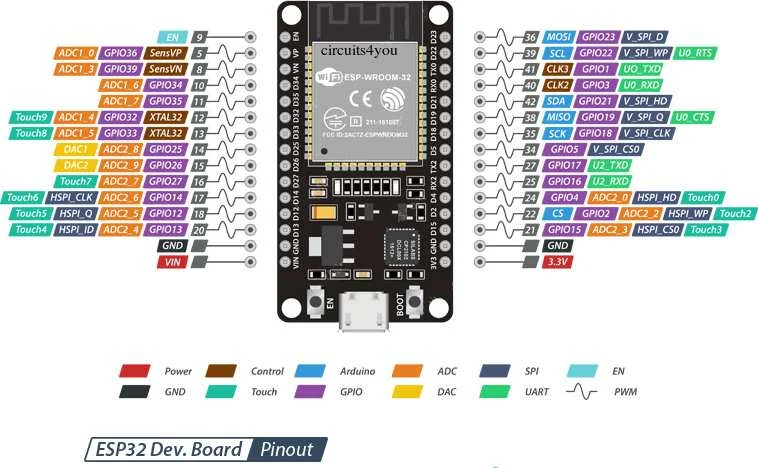
\includegraphics[width=0.8\linewidth]{imagens/esp32_pinout.png}
	\caption{Diagrama de pinagem do ESP32.}
	\label{fig:esp32_pinout}
	\vspace{0.2em}
	\small\textit{Fonte: \href{https://lastminuteengineers.com/esp32-pinout-reference/}{lastminuteengineers.com}}
\end{figure}

A escolha do ESP32 justifica-se, portanto, por sua capacidade de processamento superior, ampla conectividade, suporte a múltiplos protocolos de comunicação e integração de periféricos essenciais, reduzindo a necessidade de componentes externos. Além disso, sua popularidade na comunidade de desenvolvimento embarcado proporciona vasta documentação e bibliotecas de código, facilitando o processo de implementação e depuração do sistema. 

\section{FreeRTOS em Sistemas Embarcados}
\label{sec:freertos}

Em sistemas embarcados, especialmente aqueles que precisam lidar simultaneamente com sensoriamento, controle de atuadores, comunicação e interface com o usuário, a execução sequencial de todas as tarefas pode se tornar limitada. Nesses casos, o uso de um sistema operacional de tempo real, ou RTOS (\textit{Real-Time Operating System}), permite organizar o software em tarefas independentes, com prioridades, intervalos de execução e mecanismos de sincronização próprios.

O FreeRTOS é um sistema operacional de tempo real amplamente utilizado em microcontroladores por apresentar baixo consumo de memória, portabilidade e suporte a múltiplas arquiteturas embarcadas. Conforme apresentado por \citeonline{barry2016freertos}, o núcleo do FreeRTOS foi projetado para organizar aplicações embarcadas em tarefas concorrentes, utilizando escalonamento por prioridades e mecanismos de temporização e sincronização adequados a sistemas com recursos limitados. Diferentemente de sistemas operacionais convencionais, seu objetivo não é fornecer uma interface completa de uso geral, mas permitir a execução previsível de tarefas, como leitura de sensores, controle de motores, comunicação sem fio e atualização de estados internos do sistema.

No contexto do ESP32, o FreeRTOS é particularmente relevante, pois a própria plataforma de desenvolvimento utilizada pelo microcontrolador é baseada nesse sistema operacional. O ESP32 possui arquitetura com dois núcleos de processamento, permitindo que diferentes tarefas sejam distribuídas entre eles. Essa característica favorece a separação entre atividades críticas de controle, como leitura de encoders e atualização de comandos de motores, e atividades de comunicação, como atendimento à interface web e envio de telemetria.

Entre os principais recursos fornecidos pelo FreeRTOS estão a criação de tarefas, o escalonamento por prioridade, os atrasos temporizados, as filas de comunicação, os semáforos e os mecanismos de sincronização entre tarefas. Esses recursos permitem estruturar o software de forma modular, evitando que uma rotina bloqueante impeça a execução de outras partes importantes do sistema. Por exemplo, em um robô móvel, a leitura periódica de sensores deve ocorrer mesmo enquanto o sistema processa comandos recebidos pela interface web ou atualiza informações de monitoramento.

Neste trabalho, o uso do FreeRTOS está associado à organização das rotinas embarcadas do robô em tarefas de execução concorrente. Essa abordagem permite separar funções como aquisição de dados sensoriais, atualização da telemetria, controle de movimentação e comunicação com a interface web. Com isso, o sistema passa a responder de forma mais adequada a eventos simultâneos, como a detecção de obstáculos, a recepção de comandos externos e a necessidade de atualização contínua da posição estimada do robô.

Apesar dessas vantagens, o uso de tarefas concorrentes também exige cuidados adicionais. A troca de informações entre diferentes tarefas deve ser realizada de forma controlada, evitando condições de corrida, leituras inconsistentes ou disputas por recursos compartilhados. Por esse motivo, variáveis relacionadas ao estado do robô, leituras de sensores e comandos de movimentação devem ser tratadas com atenção, especialmente quando acessadas por múltiplas rotinas.

Assim, o FreeRTOS contribui para a organização do software embarcado ao permitir uma arquitetura baseada em tarefas, mais adequada à natureza concorrente do sistema robótico desenvolvido. Sua utilização favorece a separação entre sensoriamento, controle, navegação e comunicação, permitindo maior robustez e responsividade durante a execução dos testes experimentais.

\section{Controle de Motores DC e Ponte H} \label{sec:controle_motores}

Motores de corrente contínua (DC) são componentes amplamente utilizados em plataformas robóticas móveis, especialmente em projetos com sistemas embarcados. Isso se deve à sua construção relativamente simples, ao custo acessível e à capacidade de resposta rápida a comandos de controle. No entanto, para que seja possível controlar de forma eficaz tanto a direção quanto a velocidade desses motores, é necessário empregar circuitos de acionamento apropriados, sendo a ponte H uma das soluções mais utilizadas para esse fim.

A ponte H consiste em um arranjo eletrônico formado geralmente por quatro dispositivos semicondutores de chaveamento (transistores bipolares) dispostos de modo a formar uma topologia semelhante à letra “H”. Esse circuito permite o controle da polaridade da tensão aplicada aos terminais do motor, viabilizando, assim, o acionamento em ambos os sentidos de rotação. Tal característica é fundamental para o deslocamento de robôs autônomos, que requerem comandos precisos de avanço, recuo e curvas, os quais são obtidos por meio do controle individual de cada motor responsável pela movimentação.

Para controlar a velocidade de rotação, é frequentemente empregada a técnica de modulação por largura de pulso (PWM), que ajusta a potência média entregue ao motor pela variação do ciclo de trabalho de um sinal digital. Essa estratégia possibilita uma regulação contínua da velocidade, mantendo a eficiência energética do sistema e reduzindo o desgaste dos componentes eletromecânicos.

A ponte H, portanto, representa uma alternativa consolidada tanto em ambientes educacionais quanto em sistemas de aplicação prática, devido à sua confiabilidade e simplicidade de implementação. Sua interface com microcontroladores, como o ESP32, ocorre por meio de sinais digitais que controlam o estado de cada chave do circuito, permitindo a integração direta com algoritmos de controle embarcados.

\begin{figure}[ht]
	\centering
	\begin{subfigure}[b]{0.48\linewidth}
		\centering
		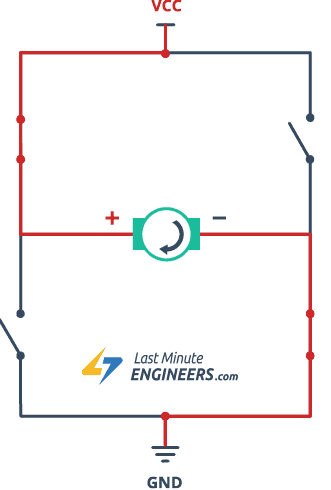
\includegraphics[width=0.7\linewidth]{imagens/ponteH_rotacao_horaria.png}
		\caption{Rotação horária do motor.}
		\label{fig:ponte_h_horario}
	\end{subfigure}
	\hfill
	\begin{subfigure}[b]{0.48\linewidth}
		\centering
		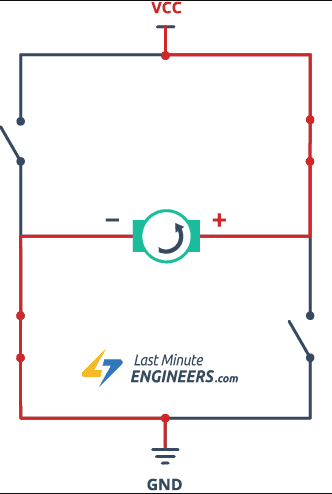
\includegraphics[width=0.7\linewidth]{imagens/ponteH_rotacao_anti_horaria.png}
		\caption{Rotação anti-horária do motor.}
		\label{fig:ponte_h_anti_horario}
	\end{subfigure}
	\caption{Funcionamento da ponte H para diferentes sentidos de rotação.}
	\label{fig:ponte_h_rotacoes}
	\vspace{0.2em}
	\small\textit{Fonte: \href{https://lastminuteengineers.com/l298n-dc-stepper-driver-arduino-tutorial/}{LASTMINUTEENGINEERS, 2024}.}
\end{figure}

A \textit{Figura~\ref{fig:ponte_h_rotacoes}} ilustra os dois modos de operação da ponte H, demonstrando como a combinação das chaves eletrônicas determina a direção da corrente elétrica no motor, resultando em rotação no sentido horário ou anti-horário.


\section{Orientação Magnética com QMC5883L} \label{sec:qmc5883l}

O QMC5883L é um magnetômetro digital de três eixos utilizado para medir componentes do campo magnético nos eixos X, Y e Z. Diferentemente de uma unidade inercial como o MPU6050, esse sensor não possui acelerômetro nem giroscópio, de modo que não fornece diretamente aceleração linear, velocidade angular ou temperatura útil para controle de movimento. Sua principal aplicação no contexto deste projeto é fornecer uma referência de orientação absoluta no plano horizontal, calculada a partir da relação entre as componentes magnéticas dos eixos X e Y.

O cálculo do ângulo de orientação, ou \textit{heading}, é realizado por meio da função \texttt{atan2}, aplicada às leituras convertidas para unidades proporcionais ao campo magnético. Após esse cálculo, podem ser aplicados ajustes de declinação magnética, offsets de calibração e normalização angular para manter o resultado em uma faixa consistente.

Matematicamente, o heading bruto obtido a partir do magnetômetro pode ser representado por:

\begin{equation}
\theta_{bruto} = \operatorname{atan2}(B_y, B_x)
\end{equation}

onde:
\begin{itemize}
\item \(B_x\) e \(B_y\) representam as componentes do campo magnético medidas nos eixos X e Y;
\item \(\operatorname{atan2}\) calcula o ângulo considerando o quadrante correto da leitura;
\item \(\theta_{bruto}\) corresponde ao heading inicial antes dos ajustes de calibração.
\end{itemize}

Após a leitura bruta, a orientação final utilizada pelo sistema é obtida pela aplicação da declinação magnética e do offset de referência angular definido no robô:

\begin{equation}
\theta_{heading} = \operatorname{mod}(\theta_{bruto} + \delta - \theta_{0},\, 360^\circ)
\end{equation}

em que \(\delta\) representa a declinação magnética local e \(\theta_{0}\) é o zero angular configurado na calibração.

Magnetômetros estão sujeitos a perturbações provocadas por materiais ferromagnéticos e por campos magnéticos gerados por correntes elétricas próximas. Por essa razão, sua aplicação em plataformas móveis exige calibração e cuidado com o posicionamento físico do sensor. As decisões específicas de integração, filtragem e uso do QMC5883L neste protótipo são apresentadas no Capítulo~\ref{cap:materiais_metodos}.

\begin{figure}[ht]
	\centering
	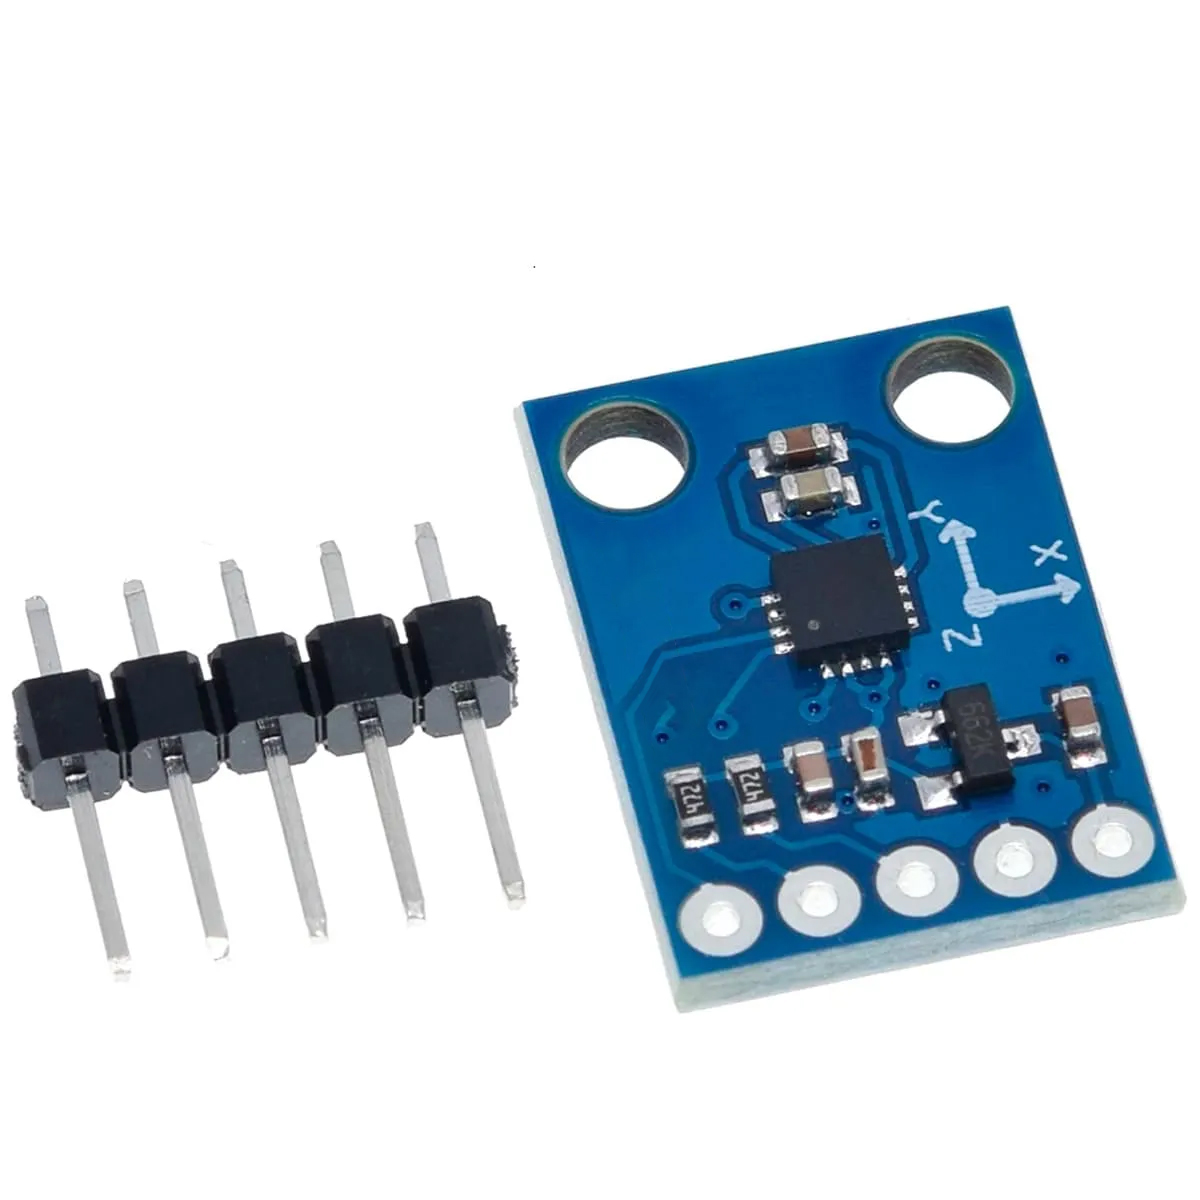
\includegraphics[width=0.55\linewidth]{imagens/qmc5883l_modulo.jpg}
	\caption{Módulo magnetômetro QMC5883L.}
	\label{fig:qmc5883l_modulo}
	\small\textit{Fonte: \href{https://www.casadarobotica.com/sensores-modulos/sensores/outros/modulo-bussola-eletronica-magnetometro-hmc5883l}{CASA DA ROBOTICA, 2026}.}
\end{figure}

\section{Sensores Time-of-Flight: VL53L0X} \label{sec:vl53l0x}
Sensores do tipo \textit{Time-of-Flight} (ToF), como o modelo VL53L0X, realizam medições de distância com base no tempo que um feixe de luz, geralmente laser infravermelho, leva para atingir um objeto e retornar ao sensor após a reflexão. Esse princípio de funcionamento permite a obtenção de leituras rápidas e com elevada precisão, alcançando uma resolução na ordem de milímetros e alcance típico de até 1,2 metros em ambientes controlados \citeonline{adafruit2024vl53l0x}. Tais características tornam os sensores ToF especialmente adequados para aplicações que requerem resposta em tempo real, como navegação autônoma, detecção e evasão de obstáculos e mapeamento de ambientes tridimensionais.

A escolha do sensor VL53L0X neste projeto se deu, principalmente, por sua superioridade em relação a outros sensores amplamente utilizados no ensino e em projetos de prototipagem, como o HC-SR04. Enquanto o HC-SR04 utiliza ondas ultrassônicas, que estão sujeitas a variações ambientais (como temperatura e tipo de superfície do objeto), o VL53L0X opera com luz, o que lhe confere maior estabilidade, tempo de resposta mais curto e maior precisão nas medições. Dessa forma, o VL53L0X apresenta-se como uma solução mais robusta e confiável para os requisitos do sistema robótico proposto, especialmente no que se refere à detecção eficiente de obstáculos em tempo real e à construção de um mapeamento preciso do ambiente. A representação de um sensor equivalente ao utilizado no projeto está representado na Figura~\ref{fig:vl53l0x-sensor}.

\begin{figure}[ht]
	\centering
	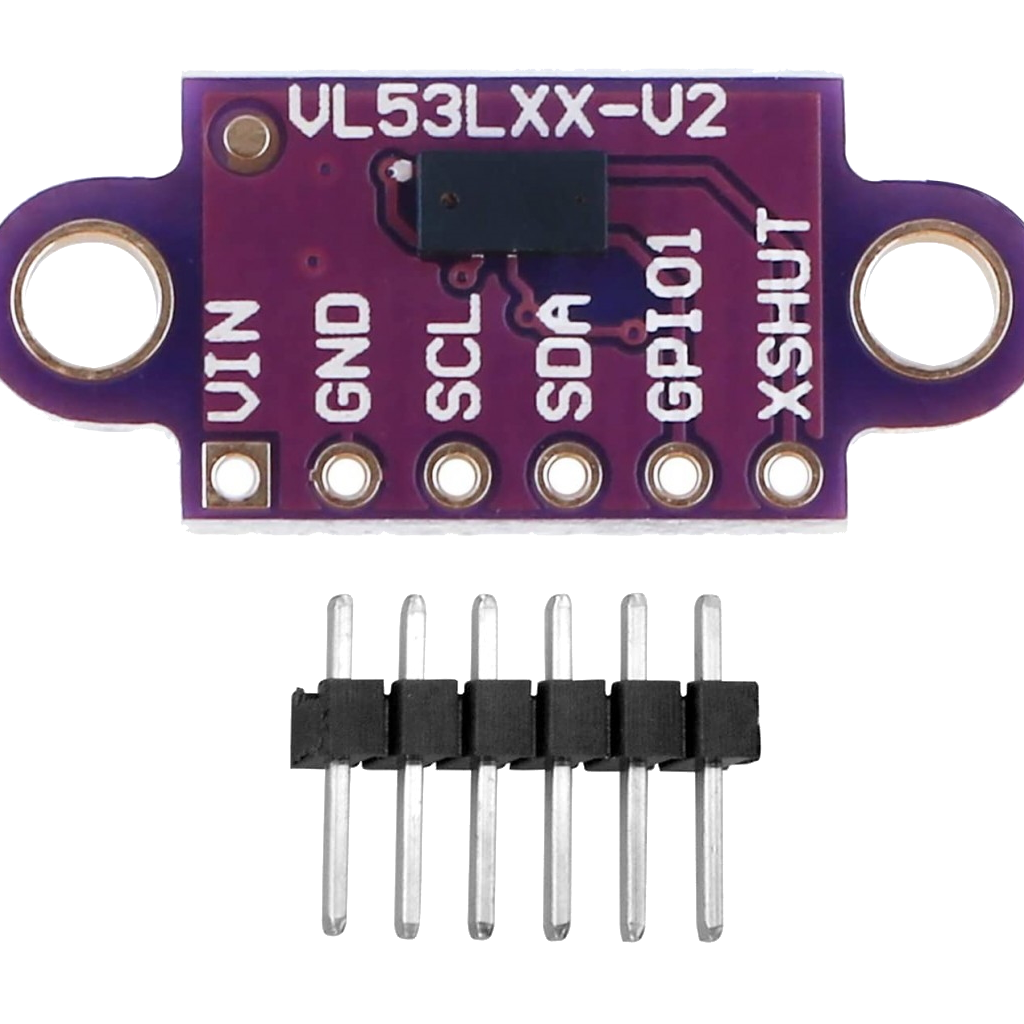
\includegraphics[width=0.5\linewidth]{imagens/VL53L0X.png}
	\caption{Sensor VL53L0X}
	\small\textit{Fonte: \href{https://arduinoecia.com.br/product/sensor-de-distancia-vl53l0x-laser-time-of-flight-tof/?srsltid=AfmBOopsNMCpEqpZlJho78S3P5lfBbjyWc4lJGDBZAgVOFW-wkH_ZL3z}{ARDUINOECIA, 2025}.}
	\label{fig:vl53l0x-sensor}
\end{figure}

\section{Algoritmos PID e Odometria} \label{sec:pid_odometria}

O controle PID é uma das técnicas mais amplamente utilizadas em sistemas de controle automático, especialmente em aplicações embarcadas e robóticas. Sua popularidade advém da simplicidade de implementação e da eficácia no controle de processos dinâmicos. Em robótica móvel, o PID é comumente aplicado ao controle de velocidade e posição dos motores, ajustando continuamente os sinais de atuação de acordo com o erro entre o valor desejado (referência) e o valor atual medido.

Matematicamente, a saída de controle \( u(t) \) do controlador PID é definida como:

\begin{equation}
u(t) = K_p e(t) + K_i \int_{0}^{t} e(\tau)\, d\tau + K_d \frac{de(t)}{dt}
\end{equation}

onde:
\begin{itemize}
	\item \( e(t) \) representa o erro entre a referência e a saída do sistema no instante \( t \);
	\item \( K_p \) é o ganho proporcional, que reage à magnitude do erro atual;
	\item \( K_i \) é o ganho integral, que corrige desvios acumulados ao longo do tempo;
	\item \( K_d \) é o ganho derivativo, que antecipa tendências com base na taxa de variação do erro.
\end{itemize}

A sintonização adequada desses parâmetros (\( K_p \), \( K_i \) e \( K_d \)) é essencial para garantir estabilidade, tempo de resposta adequado e evitar oscilações ou sobrecargas no sistema, como mostrado em \citeonline{astrom2006advancedpid}.

Complementarmente ao controle, a navegação precisa em ambientes internos exige a estimativa contínua da posição e da orientação do robô, processo conhecido como odometria. A odometria clássica baseia-se na leitura incremental dos encoders ópticos acoplados às rodas motrizes, que fornecem a quantidade de pulsos gerados conforme as rodas giram. Com base nesses dados, é possível calcular o deslocamento linear e angular do robô por integração das variações de posição ao longo do tempo.

Considerando um robô diferencial com duas rodas, os deslocamentos linear \( \Delta s \) e angular \( \Delta \theta \) são dados por: \citeonline{siegwart2011introduction}

\begin{align}
	\Delta s &= \frac{r}{2} (\Delta \phi_R + \Delta \phi_L) \\
	\Delta \theta &= \frac{r}{d} (\Delta \phi_R - \Delta \phi_L)
\end{align}

onde:
\begin{itemize}
	\item \( r \) é o raio das rodas;
	\item \( d \) é a distância entre as rodas;
	\item \( \Delta \phi_R \) e \( \Delta \phi_L \) são os incrementos angulares das rodas direita e esquerda, respectivamente.
\end{itemize}

Essas equações permitem atualizar a posição do robô em coordenadas cartesianas \( (x, y) \) com base no deslocamento linear e na mudança de orientação, utilizando relações trigonométricas.

Apesar da sua simplicidade, a odometria baseada exclusivamente em encoders está sujeita a erros cumulativos, como deslizamentos de roda e imprecisões de leitura. Para mitigar esses erros, é comum a fusão de sensores, combinando odometria com referências externas de orientação, como o \textit{magnetômetro QMC5883L} \cite{unicamp2017odometria}.

Portanto, a utilização combinada do controle PID e da odometria fornece uma base robusta para a movimentação precisa e a navegação confiável do robô em ambientes internos, atendendo aos requisitos de autonomia e estabilidade do sistema proposto.

\section{Mapeamento em Grid e Planejamento de Rotas}
\label{sec:mapeamento_grid}

O mapeamento em grid é uma técnica amplamente adotada na robótica móvel para representar ambientes de maneira discreta. Nessa abordagem, o espaço contínuo é dividido em uma matriz bidimensional de células uniformes, também denominada grade de ocupação. Cada célula representa uma região do ambiente e pode ser classificada, por exemplo, como livre, ocupada ou desconhecida, de acordo com as informações disponíveis sobre o espaço \cite{ufla2020mapa}.

A representação matricial facilita o tratamento computacional do ambiente e permite formular o problema de navegação como uma busca em grafo. As células livres correspondem aos estados que podem ser visitados pelo robô, enquanto as células ocupadas restringem o conjunto de movimentos admissíveis. A Figura~\ref{fig:grid-mapping-basics} apresenta um exemplo de discretização de um ambiente em células.

\begin{figure}[ht]
		\centering
		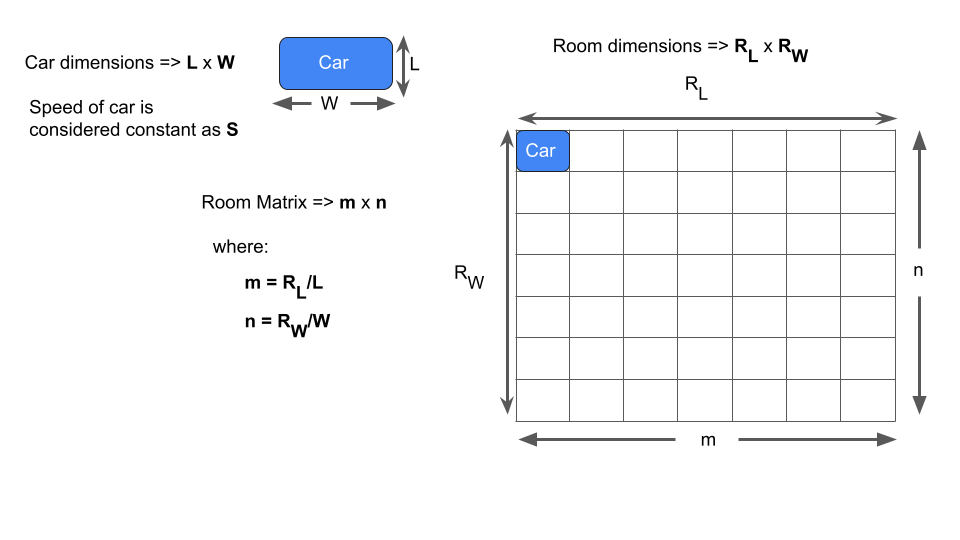
\includegraphics[width=0.9\linewidth]{imagens/grid_mapping_basics.png}
		\caption{Exemplo simplificado de mapeamento em grid \cite{patel2021ultrasonic}.}
		\label{fig:grid-mapping-basics}
\end{figure}

Após a definição da grade, algoritmos de busca podem ser empregados para calcular uma trajetória entre uma célula inicial e uma célula de destino. Entre os algoritmos utilizados para esse propósito estão Dijkstra e A*. O algoritmo A* combina o custo acumulado desde a origem com uma função heurística que estima o custo restante até o destino.

De forma geral, a função de avaliação do A* é expressa por:

\begin{equation}
		f(n) = g(n) + h(n),
\end{equation}

em que \(g(n)\) representa o custo acumulado da origem até o nó \(n\), e \(h(n)\) representa uma estimativa do custo entre \(n\) e o destino. Em grades com movimentação ortogonal, uma heurística comum é a distância de Manhattan.

A rota gerada pelo planejador é formada por uma sequência ordenada de células adjacentes. Para que essa rota seja executada por um robô móvel, ela deve ser convertida em comandos de movimento compatíveis com sua cinemática. A definição do mapa utilizado, da posição inicial, da forma de informar o destino e das modificações realizadas no algoritmo A* pertence à implementação deste trabalho e, por isso, é apresentada no Capítulo~\ref{cap:materiais_metodos}.

\chapter{Materiais e Métodos}
\label{cap:materiais_metodos}

Este capítulo descreve, de maneira detalhada, os materiais empregados e os procedimentos metodológicos adotados para o desenvolvimento do protótipo de robô autônomo proposto. A escolha criteriosa dos componentes eletrônicos, sensores e atuadores foi orientada pelas necessidades do sistema, levando em consideração fatores como precisão, custo, disponibilidade e compatibilidade com a plataforma de desenvolvimento utilizada.

São apresentados o ambiente de desenvolvimento de software, as bibliotecas utilizadas, os recursos computacionais embarcados, bem como a lógica de controle implementada no microcontrolador. A metodologia abrange também a integração dos sensores, o controle dos motores, o modelo de mapeamento em grid e a abordagem utilizada para planejamento de rotas.

\section{Arquitetura do Sistema e Prototipagem de Hardware}
\label{sec:arquitetura_sistema}

A arquitetura do sistema foi definida com o objetivo de integrar, de maneira modular, os componentes de sensoriamento, processamento, atuação, alimentação elétrica e interface com o usuário necessários para o funcionamento autônomo do robô móvel. Essa organização permite compreender o sistema não apenas como um conjunto de componentes eletrônicos isolados, mas como uma estrutura embarcada integrada, na qual os dados coletados pelos sensores são processados pelo microcontrolador e convertidos em comandos de controle para os motores.

A Figura~\ref{fig:arquitetura_sistema} apresenta a arquitetura geral adotada no projeto, destacando os principais módulos utilizados e os fluxos de dados, controle e alimentação elétrica entre eles.

\begin{figure}[ht]
	\centering
	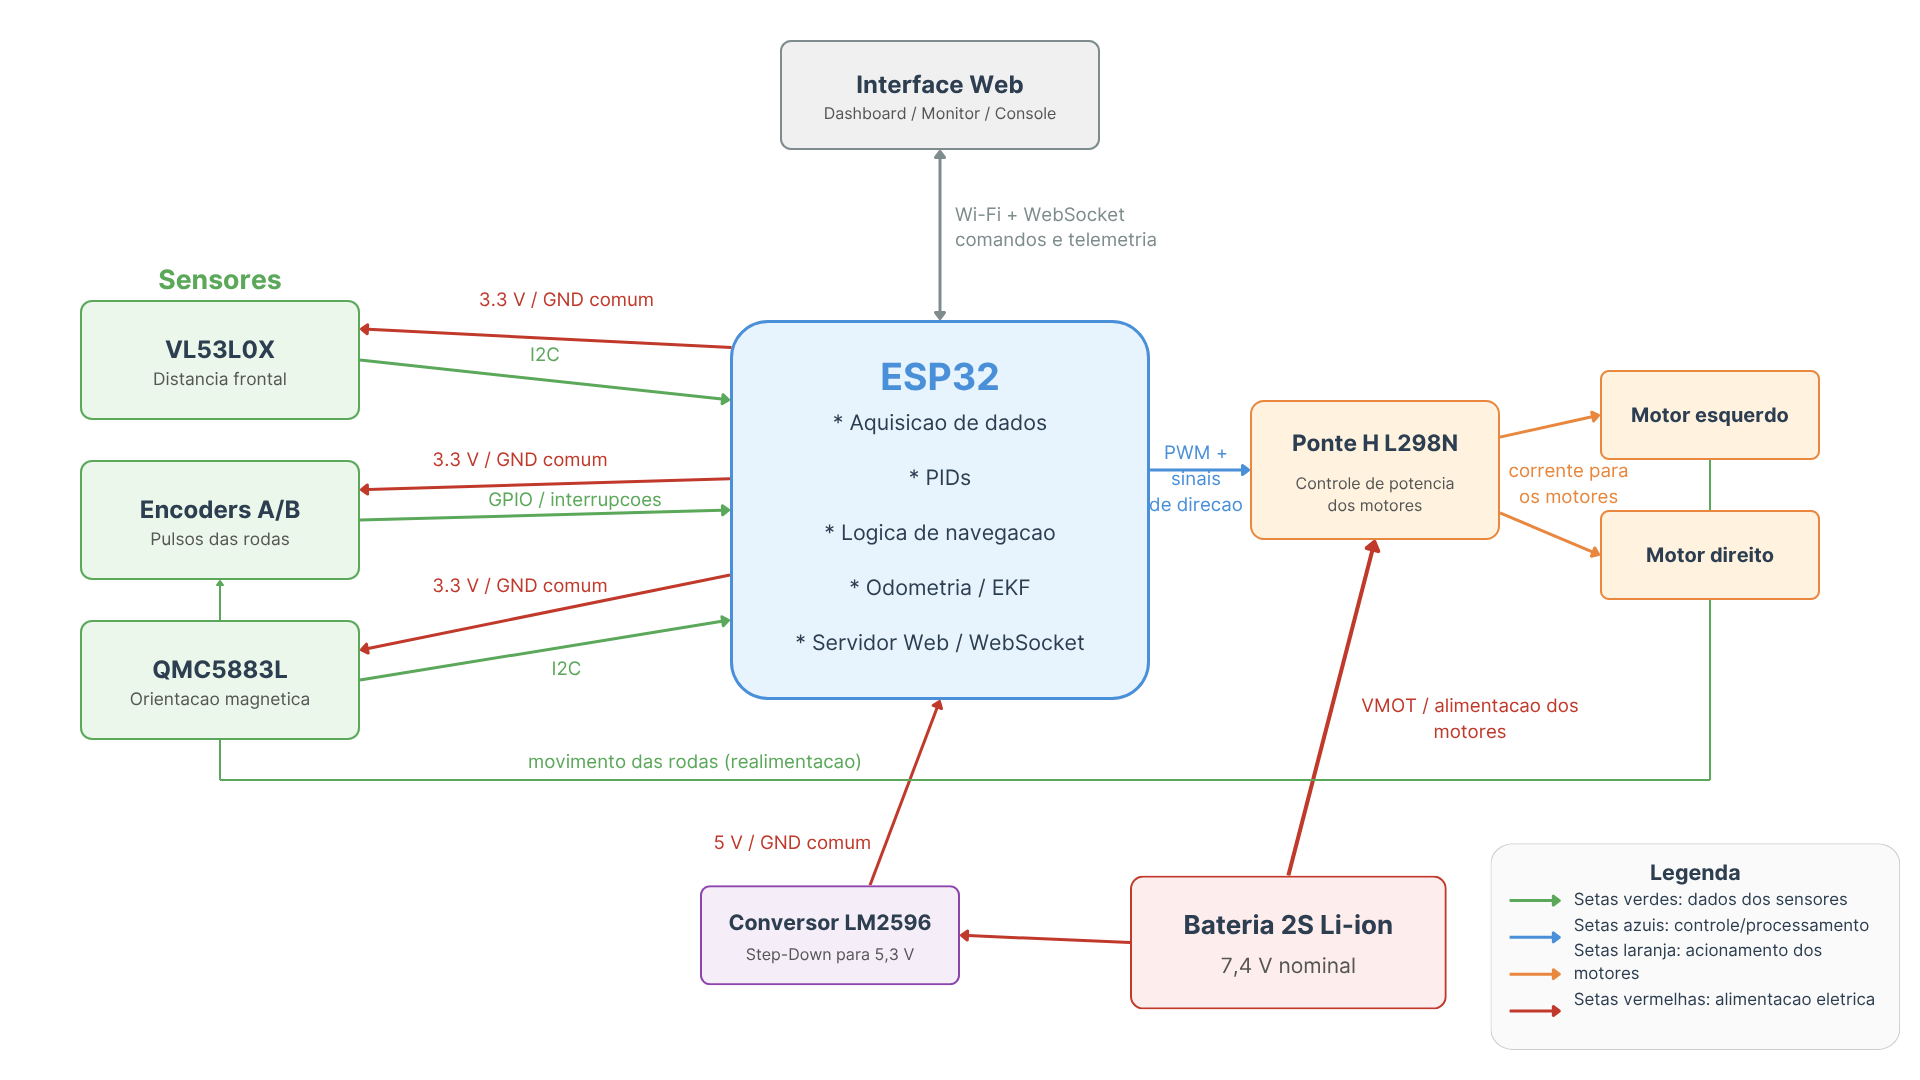
\includegraphics[width=0.95\linewidth]{imagens/arquitetura_sistema.png}
	\caption{Arquitetura geral do sistema robótico embarcado.}
	\label{fig:arquitetura_sistema}
\end{figure}

Conforme ilustrado na Figura~\ref{fig:arquitetura_sistema}, o ESP32 atua como unidade central de processamento do robô. Esse microcontrolador é responsável pela aquisição dos dados dos sensores, pelo tratamento das leituras recebidas, pela execução da lógica de navegação, pelo controle dos motores e pela comunicação com a interface web. A escolha do ESP32 está relacionada à sua capacidade de processamento, à disponibilidade de interfaces de comunicação, ao suporte a interrupções para leitura dos encoders e à conectividade Wi-Fi integrada, características discutidas na fundamentação teórica e aproveitadas diretamente na implementação do sistema.

O módulo de sensoriamento é composto principalmente pelos encoders ópticos, pelo sensor de distância VL53L0X e pelo magnetômetro QMC5883L. Os encoders fornecem pulsos associados à rotação das rodas, permitindo estimar o deslocamento do robô, calcular a odometria e controlar os movimentos lineares e angulares. O sensor VL53L0X, baseado em tecnologia \textit{Time-of-Flight}, é utilizado para medir a distância frontal e identificar obstáculos durante a navegação. Já o QMC5883L fornece uma referência auxiliar de orientação magnética no plano horizontal, sendo empregado para estimativa do \textit{heading} quando suas leituras apresentam estabilidade suficiente.

A partir das informações sensoriais, o ESP32 executa rotinas de controle e decisão, incluindo controladores PID, lógica de navegação em grid, planejamento de movimento entre células, monitoramento de obstáculos e atualização da posição estimada do robô. Essas informações são utilizadas para gerar sinais de controle enviados ao módulo Ponte H L298N. A Ponte H recebe sinais digitais e PWM do ESP32 e realiza o acionamento elétrico dos motores de corrente contínua, permitindo o controle independente dos lados esquerdo e direito do robô.

A estrutura física do robô é baseada em uma plataforma de quatro rodas acionadas por motores de corrente contínua. Cada lado possui dois motores conectados em paralelo, formando dois conjuntos de tração: um conjunto esquerdo e um conjunto direito. Essa configuração permite a locomoção diferencial do robô, possibilitando movimentos de avanço, ré e rotação sobre o próprio eixo. Os motores frontais são equipados com encoders, utilizados como principal fonte de realimentação para o controle de deslocamento e rotação.

O sistema de alimentação foi organizado de forma a separar a alimentação de potência dos motores da alimentação lógica dos circuitos de controle e sensoriamento. A bateria Li-ion 2S, com tensão nominal de $7{,}4\,\text{V}$, alimenta diretamente a Ponte H L298N, responsável pelo fornecimento de corrente aos motores. Em paralelo, a mesma bateria alimenta um conversor regulador LM2596, responsável por fornecer uma tensão regulada de $5\,\text{V}$ para o ESP32 e os sensores. Todos os módulos compartilham uma referência comum de GND, condição necessária para o funcionamento adequado dos sinais de controle e comunicação entre os componentes.

A interface com o usuário é realizada por meio de uma interface web embarcada no ESP32, acessível via rede Wi-Fi local. Essa interface permite enviar comandos ao robô, selecionar destinos no mapa, acompanhar a telemetria, visualizar leituras dos sensores, observar a pose estimada do robô e consultar mensagens de registro do sistema. A troca de informações entre a interface e o microcontrolador ocorre por meio de WebSockets e mensagens em formato JSON, permitindo comunicação bidirecional em tempo real.

Dessa forma, a arquitetura adotada estabelece um ciclo de realimentação entre sensoriamento, processamento e atuação. Os sensores informam o estado físico do robô e do ambiente, o ESP32 processa essas informações e define as ações de controle, a Ponte H converte os comandos em acionamento elétrico dos motores, e a interface web permite o monitoramento e a interação com o sistema durante os testes.

\subsection{Prototipagem e Ajustes de Hardware}
\label{sec:prototipagem_ajustes}

Após a definição da arquitetura geral, os componentes foram organizados em uma montagem de prototipagem para validar, de forma prática, a integração entre os módulos apresentados na fundamentação teórica. Essa etapa permitiu verificar a compatibilidade entre o ESP32, a Ponte H L298N, os motores DC, os encoders, o sensor VL53L0X, o magnetômetro QMC5883L, o conversor LM2596 e o sistema de alimentação por bateria.

A Figura~\ref{fig:protoboard_model_v2} apresenta a organização física revisada dos componentes em ambiente de prototipação. Essa representação foi utilizada como referência para a montagem do protótipo, evidenciando a disposição dos módulos principais, das conexões de alimentação e dos sinais de controle.

\begin{figure}[ht]
	\centering
	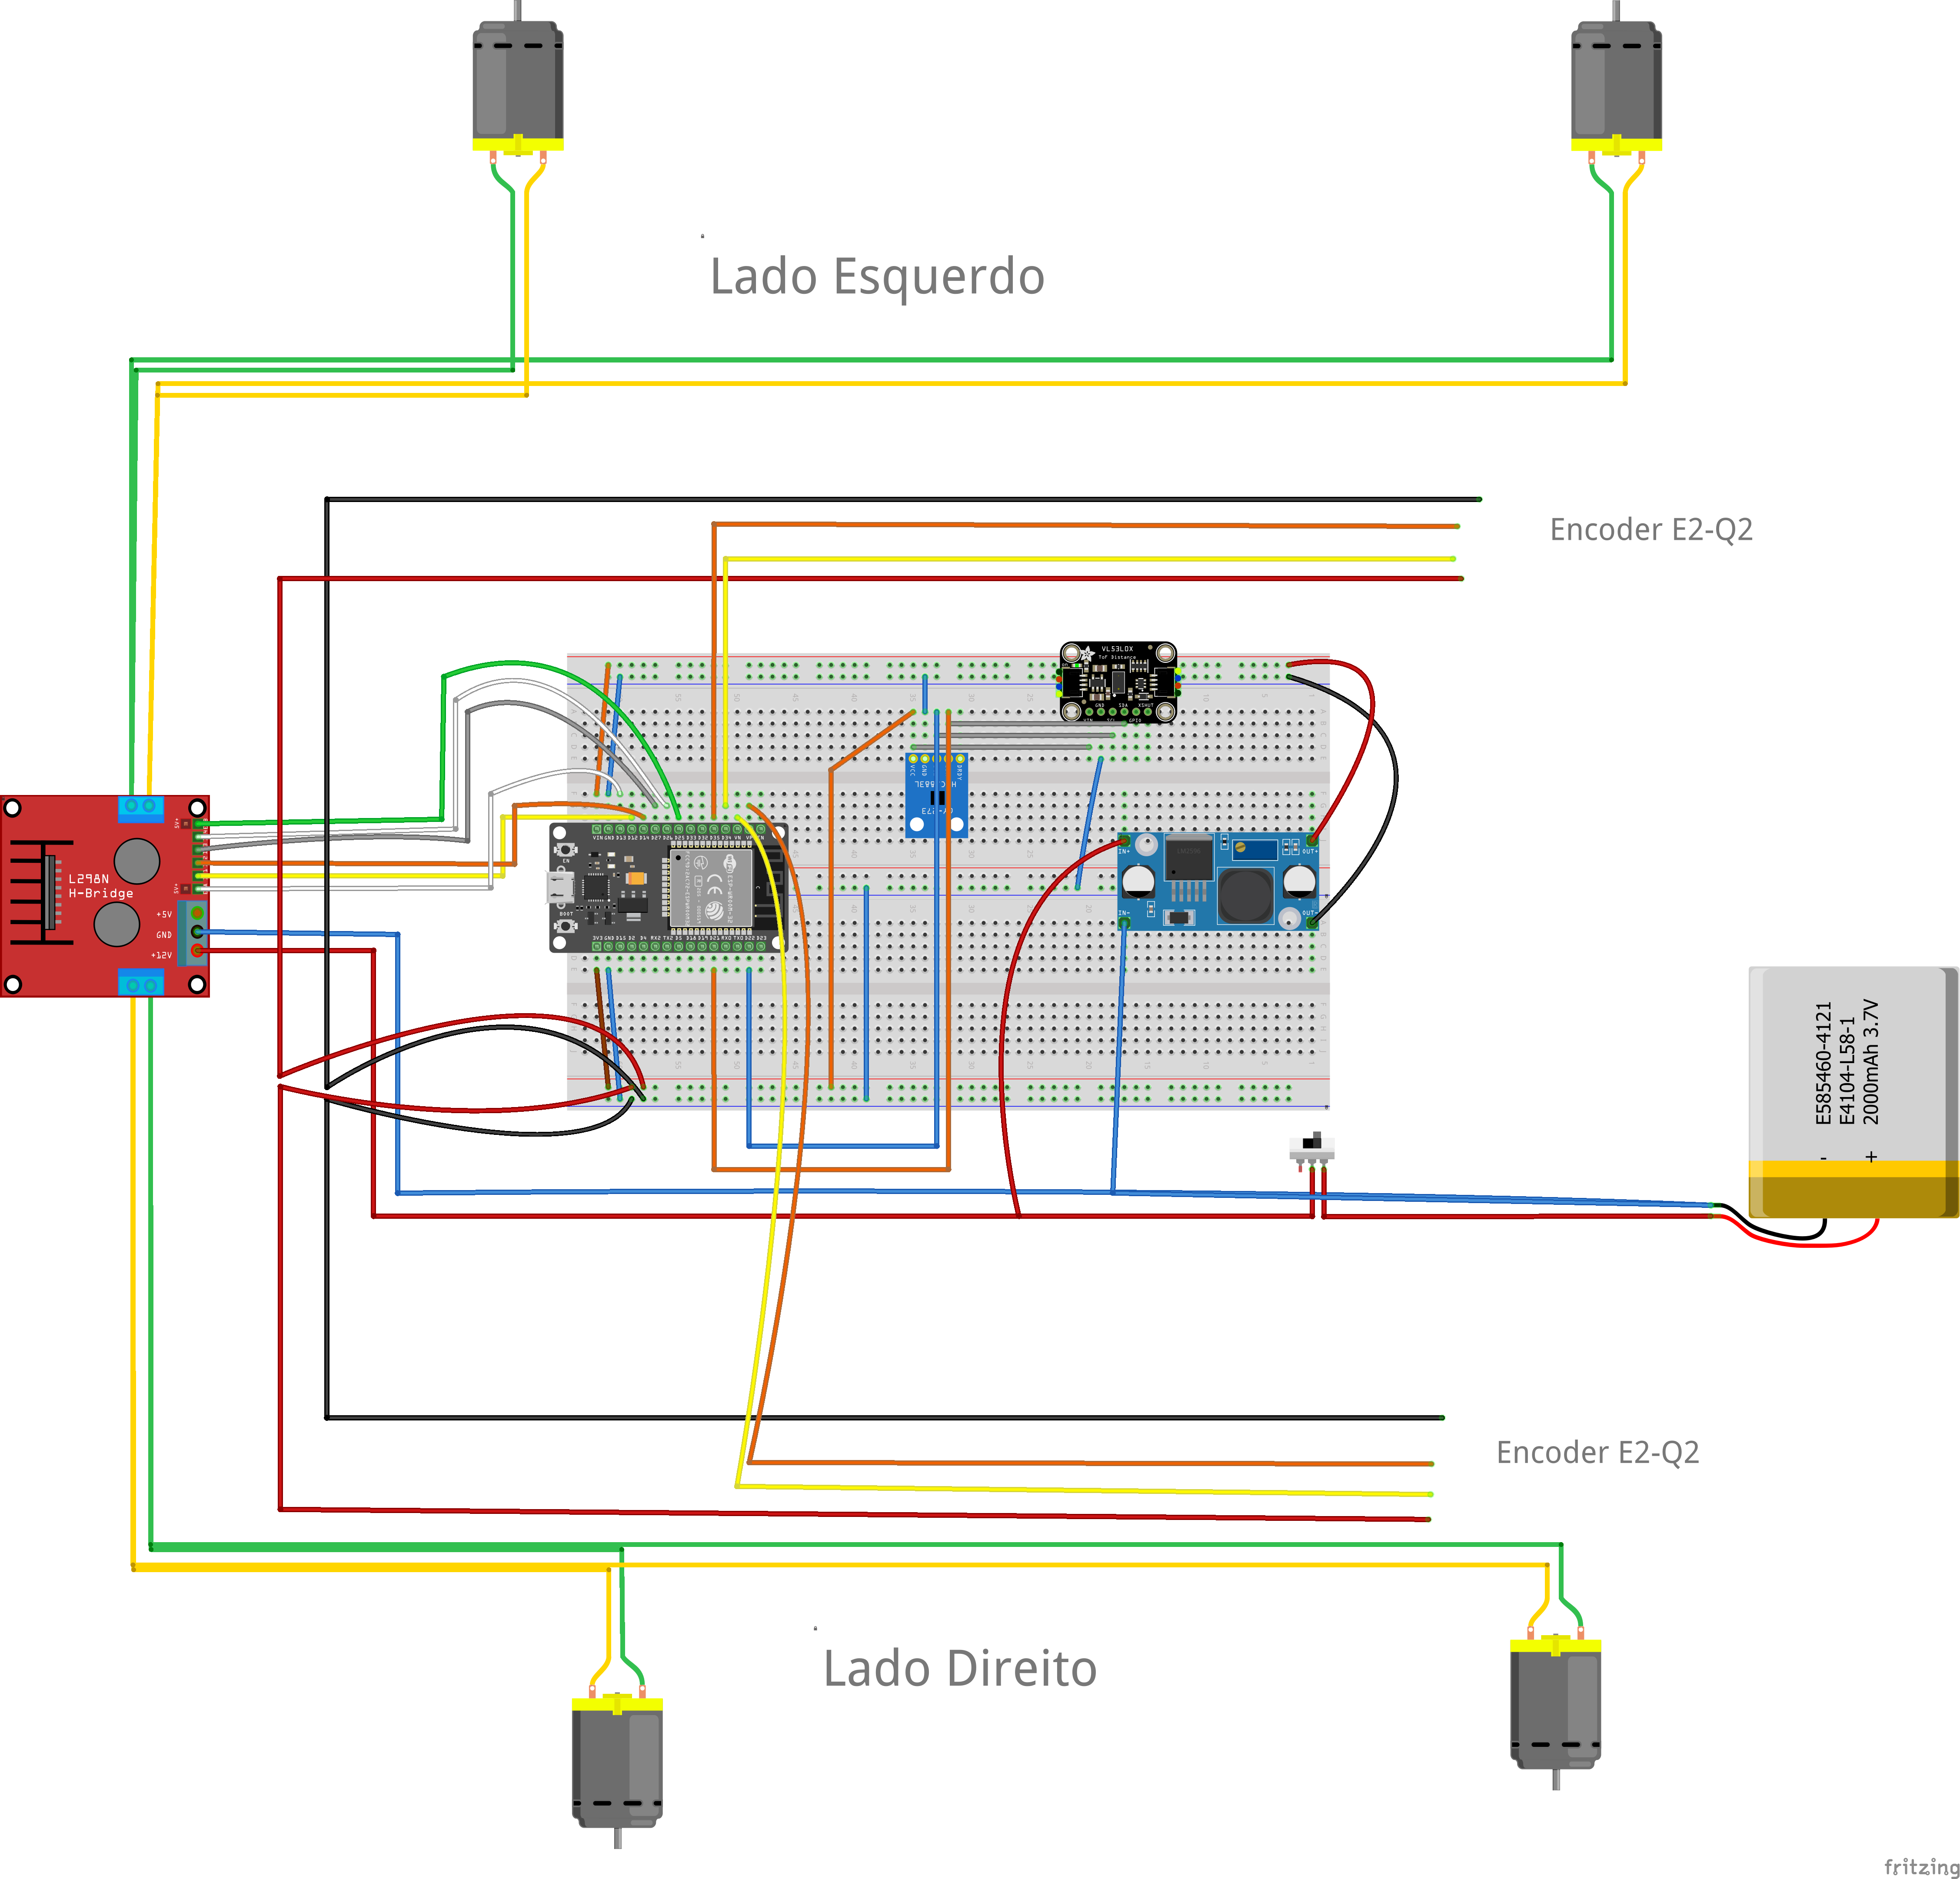
\includegraphics[width=0.75\linewidth]{imagens/Protoboard_ESPCar_v2.png}
	\caption{Organização revisada dos componentes utilizados no protótipo do robô móvel.}
	\small Modelo desenvolvido com auxílio da ferramenta \href{https://fritzing.org/}{Fritzing.org}.
	\label{fig:protoboard_model_v2}
\end{figure}

Durante os testes de integração, foram realizados ajustes na disposição dos componentes e no roteamento das conexões, buscando reduzir desconexões, facilitar a manutenção e melhorar a estabilidade elétrica do sistema durante a movimentação do robô. A separação entre a alimentação dos motores e a alimentação do ESP32 e sensores foi um ponto importante dessa etapa, pois os motores podem introduzir ruídos e quedas de tensão capazes de afetar o funcionamento dos circuitos lógicos.

Também foram observadas limitações práticas associadas ao uso do magnetômetro QMC5883L. Embora o sensor tenha sido incorporado como referência auxiliar de orientação, os testes indicaram que suas leituras podem sofrer interferências causadas por motores, correntes elétricas, fios de alimentação e componentes metálicos próximos. Por esse motivo, os encoders permaneceram como principal fonte de informação para controle de deslocamento e rotação, enquanto o QMC5883L foi tratado como uma referência complementar, utilizada apenas quando suas leituras apresentavam estabilidade suficiente.

Na implementação do firmware, o \textit{heading} foi calculado a partir das componentes magnéticas dos eixos X e Y, com uso de offset para definição do zero angular e normalização da leitura. Também foram aplicados critérios de rejeição para descartar variações incompatíveis com a movimentação esperada. Essas decisões pertencem à metodologia de integração do sensor no protótipo, enquanto os efeitos observados durante os testes são discutidos no Capítulo~\ref{chap:resultados}.

A etapa de prototipagem, portanto, permitiu consolidar a arquitetura de hardware utilizada no projeto, aproximando os conceitos discutidos na fundamentação teórica da implementação física do robô. Além disso, os ajustes realizados nessa fase contribuíram diretamente para a execução dos testes de navegação em grid, deslocamento entre células, detecção de obstáculos, controle por encoders e monitoramento remoto por interface web.

O circuito foi montado sobre um chassi de acrílico, mostrado na Figura~\ref{fig:robo_original}. As rodas são acionadas em duplas, direita e esquerda, por dois canais independentes da ponte H. Dessa forma, um robô com rodas diferenciais é implementado.

\begin{figure}[ht]
	\centering
	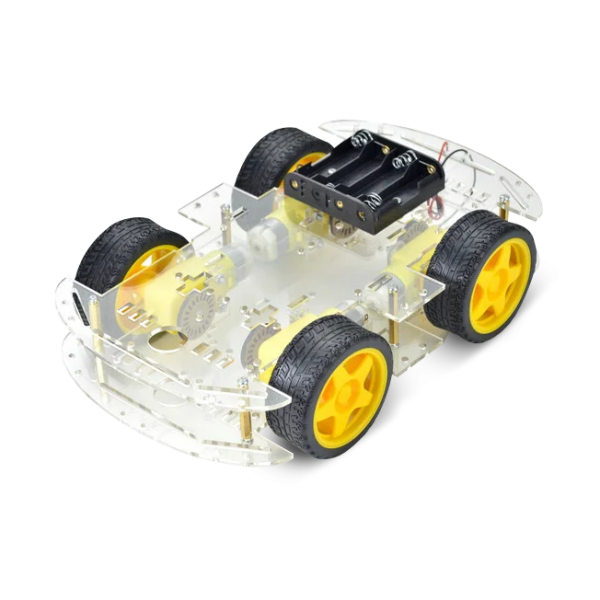
\includegraphics[width=0.75\linewidth]{imagens/Imagem_Carrinho_Acrilico.png}
	\caption{Conjunto original do carrinho, com chassi de acrílico, motores DC e Porta 4 pilhas.}
	\small\textit{Fonte: \href{https://www.robocore.net/kit-plataforma-robotica/kit-chassi-4wd-com-motores-e-rodas/}{Robocore.net}}
	\label{fig:robo_original}
\end{figure}

Concluída a etapa de integração, o protótipo físico foi utilizado nos ensaios descritos neste capítulo. As fotografias e a discussão da montagem final são apresentadas no Capítulo~\ref{chap:resultados}, na Seção~\ref{sec:resultados_montagem_final}, pois constituem resultados do desenvolvimento realizado.

\section{Integração e Montagem Mecânica do Robô}

O chassi do robô foi projetado e montado utilizando materiais leves e resistentes, priorizando a eficiência energética e a mobilidade. As rodas foram acopladas a motores de corrente contínua equipados com encoders rotativos, permitindo o controle preciso da velocidade e do deslocamento, fundamentais para a implementação de algoritmos de navegação autônoma.

Os sensores foram posicionados de acordo com suas funções no sistema. O sensor ToF foi colocado na região frontal do chassi para realizar medições no sentido de deslocamento. O magnetômetro QMC5883L foi instalado buscando o maior afastamento possível da ponte H, dos motores, da bateria e dos cabos de corrente elevada. A fiação foi organizada e fixada para facilitar a manutenção, reduzir movimentos dos conectores e diminuir a exposição do sensor magnético às fontes de interferência presentes no protótipo.

A alimentação do sistema é fornecida por uma bateria de íon-lítio (Li-ion) 2S, escolhida por sua densidade energética e capacidade de recarga. A distribuição de energia foi organizada com conector XT60, chave SS12F46, regulador LM2596 e módulo L298N. A versão avaliada permaneceu montada sobre protoboard e conexões por jumpers, configuração utilizada durante os ensaios experimentais.


\section{Ambiente de Desenvolvimento}
\label{sec:dev_ide}

O desenvolvimento do \textit{firmware} embarcado do robô autônomo foi realizado no \textit{Visual Studio Code}, utilizando a extensão PlatformIO e o \textit{framework} Arduino para ESP32. Essa escolha permitiu organizar o projeto em uma estrutura modular, com separação entre código-fonte, bibliotecas customizadas, arquivos de interface web e configurações de compilação.

O uso do PlatformIO facilitou o gerenciamento das dependências, a configuração da placa ESP32, a compilação do projeto e o envio dos arquivos estáticos da interface para a memória flash do microcontrolador. Como a interface web é composta por arquivos HTML, CSS e JavaScript, o suporte a sistemas de arquivos embarcados, como SPIFFS, tornou-se parte importante do fluxo de desenvolvimento.

Além da organização do código, o ambiente também favoreceu a depuração incremental. Durante o desenvolvimento, logs via serial e via interface web foram utilizados para acompanhar leituras dos encoders, estado do magnetômetro, detecção de obstáculos, planejamento de rota, execução de células e calibração de curvas.

\subsection{Execução concorrente com FreeRTOS}

Embora o desenvolvimento do \textit{firmware} tenha sido realizado com o \textit{framework} Arduino para ESP32, a execução das rotinas no microcontrolador ocorre sobre a infraestrutura do FreeRTOS, conforme discutido na Seção~\ref{sec:freertos}. No projeto, essa característica foi explorada para organizar partes do sistema em tarefas concorrentes, separando rotinas com responsabilidades distintas, como leitura de sensores, atualização de telemetria, comunicação com a interface web e controle de movimentação.

Essa organização foi importante para manter a responsividade do robô durante a navegação. Em um sistema móvel autônomo, o controle dos motores e a leitura dos sensores não podem depender exclusivamente de uma execução sequencial bloqueante, pois atrasos em uma rotina poderiam comprometer a detecção de obstáculos, o envio de dados à interface ou a atualização da posição estimada. Assim, a divisão em tarefas contribuiu para que o sistema continuasse processando informações de sensoriamento e comunicação enquanto executava comandos de movimento.

No contexto deste trabalho, o uso do FreeRTOS favoreceu a separação entre aquisição de dados, controle de baixo nível, comunicação com o usuário e registro de eventos. Essa abordagem também facilitou os testes incrementais do sistema, uma vez que permitiu isolar responsabilidades do \textit{firmware} e acompanhar o comportamento de cada módulo durante a execução experimental.

\subsection{Bibliotecas Utilizadas}

Para a implementação das funcionalidades do sistema embarcado, foram utilizadas bibliotecas tanto nativas quanto de terceiros. Essas bibliotecas atuaram na abstração de protocolos de comunicação, controle de hardware, gerenciamento de rede e suporte à interface web. A Tabela~\ref{tab:libs_oficiais} apresenta as principais bibliotecas utilizadas e suas respectivas finalidades.

\begin{table}[ht]
	\centering
	\caption{Bibliotecas externas e oficiais utilizadas no projeto}
	\label{tab:libs_oficiais}
	\begin{tabular}{|p{5cm}|p{10cm}|}
		\hline
		\textbf{Biblioteca} & \textbf{Finalidade} \\
		\hline
		\texttt{Wire.h} & Comunicação I2C com sensores como QMC5883L e VL53L0X. \\
		\texttt{Arduino.h} & Funções básicas de controle de pinos, temporização e compatibilidade com o ecossistema Arduino. \\
		\texttt{FreeRTOS} & Infraestrutura de execução concorrente disponível no ESP32, utilizada para criação e organização de tarefas do sistema embarcado. \\
		\texttt{math.h} & Cálculos matemáticos, incluindo trigonometria e manipulação de ponto flutuante. \\
		\texttt{ArduinoJson.h} & Criação e interpretação de objetos JSON para comunicação com a interface web. \\
		\texttt{WiFi.h} & Conexão do ESP32 à rede Wi-Fi local. \\
		\texttt{ESPAsyncWebServer.h} & Criação de servidor web assíncrono, com suporte a múltiplas conexões simultâneas. \\
		\texttt{SPIFFS.h} & Leitura e escrita dos arquivos da interface web no sistema de arquivos embarcado. \\
		\texttt{Adafruit\_VL53L0X.h} & Controle do sensor de distância VL53L0X. \\
		\texttt{Adafruit\_Sensor.h} & Interface comum para sensores Adafruit. \\
		\texttt{QMC5883L\_Custom} & Biblioteca própria para configuração, leitura e filtragem do magnetômetro QMC5883L. \\
		\hline
	\end{tabular}
\end{table}

Durante as primeiras versões do sistema, foi avaliada a utilização de resolução local de nome por DNS/mDNS, de modo que a interface web pudesse ser acessada por um endereço amigável na rede local. Entretanto, nos testes práticos, esse recurso não se mostrou suficientemente útil ou consistente em diferentes cenários de conexão, especialmente quando o acesso era realizado por meio de rede compartilhada pelo roteador do celular. Por esse motivo, a abordagem foi removida da versão final, optando-se pelo acesso direto ao endereço IP atribuído ao ESP32 pelo roteador. Essa decisão simplificou a conexão com a interface web e reduziu uma dependência adicional da camada de rede.

\subsection{Bibliotecas Customizadas}

A fim de modularizar o sistema, reduzir a complexidade do código-fonte principal e facilitar a manutenção e reuso de funcionalidades, diversas bibliotecas personalizadas foram desenvolvidas especificamente para o projeto. Essas bibliotecas encapsulam funcionalidades críticas como controle de motores, leitura de sensores, filtragem de sinais e gerenciamento de energia. A seguir, são listadas as bibliotecas customizadas implementadas:

\begin{itemize}
		\item \textbf{PID}: Implementa o algoritmo de controle Proporcional–Integral–Derivativo, permitindo múltiplas instâncias com parâmetros distintos. Essencial para o controle de velocidade dos motores com base em dados de odometria.

		\item \textbf{Filtros e validações}: Realizam suavização e validação de leituras, incluindo rejeição de amostras anômalas do QMC5883L e de saltos incompatíveis dos encoders.

		\item \textbf{Encoder}: Abstrai a leitura dos encoders das rodas, permitindo o cálculo da velocidade, do deslocamento linear e da rotação estimada durante curvas.

		\item \textbf{Monitoramento e logs}: Agrupa rotinas de diagnóstico utilizadas para registrar telemetria, estado de navegação, erros de sensores e eventos relevantes para calibração.

		\item \textbf{VL53L0X (custom)}: Estende a biblioteca oficial com lógica adicional para detecção de obstáculos com limiares configuráveis.

		\item \textbf{QMC5883L (custom)}: Integra a configuração do magnetômetro, a leitura dos eixos X, Y e Z, o cálculo de \textit{heading}, a aplicação de offset angular e a rejeição de leituras instáveis.

		\item \textbf{Motor}: Controla individualmente cada motor, centralizando a lógica de PWM, leitura de encoder e resposta ao PID.

		\item \textbf{PonteH}: Biblioteca de alto nível responsável pelo controle simultâneo dos motores do robô. Gerencia comandos de movimento, como deslocamento linear, curvas e manobras de rotação no próprio eixo. Também integra informações de sensores para ajuste de trajetória e comunicação em tempo real com a interface web.
\end{itemize}

A combinação dessas bibliotecas permitiu uma separação clara entre as responsabilidades de cada módulo do sistema, promovendo um desenvolvimento mais organizado, escalável e de fácil manutenção.

\section{Estratégias de Controle e Navegação}
\label{sec:controle_navegacao}

A navegação autônoma do robô é composta por um conjunto de estratégias interligadas que envolvem sensoriamento, controle de movimento, estimativa de posição e planejamento de trajetória. O sistema foi projetado para operar de forma reativa e deliberativa, ou seja, combinando a coleta contínua de dados do ambiente com decisões de alto nível baseadas em um mapa interno.

\subsection{Odometria e Estimativa de Posição}

A estimativa de deslocamento do robô é realizada por meio da odometria diferencial, utilizando a contagem de pulsos dos encoders ópticos instalados nas rodas frontais. Esses dados são processados para determinar a distância percorrida por cada lado do robô e a variação angular ao longo do tempo. Como o robô utiliza uma configuração de tração diferencial, na qual os lados esquerdo e direito podem ser acionados de forma independente, a pose do robô pode ser estimada a partir da diferença entre os deslocamentos das rodas.

Inicialmente, os pulsos acumulados pelos encoders são convertidos em deslocamento linear. Considerando uma roda de raio $r$, uma resolução de encoder de $N$ pulsos por volta e variações de contagem $\Delta p_L$ e $\Delta p_R$ para as rodas esquerda e direita, respectivamente, os deslocamentos lineares de cada lado são calculados pelas Equações~\ref{eq:deslocamento_roda_esquerda} e~\ref{eq:deslocamento_roda_direita}:
\begin{equation}
	\Delta s_L = \frac{2\pi r}{N}\Delta p_L
	\label{eq:deslocamento_roda_esquerda}
\end{equation}
\begin{equation}
	\Delta s_R = \frac{2\pi r}{N}\Delta p_R
	\label{eq:deslocamento_roda_direita}
\end{equation}
Em seguida, o deslocamento médio do robô e sua variação angular são obtidos, respectivamente, pelas Equações~\ref{eq:deslocamento_medio} e~\ref{eq:variacao_angular_odometria}, de acordo com o modelo cinemático diferencial:
\begin{equation}
	\Delta s = \frac{\Delta s_R + \Delta s_L}{2}
	\label{eq:deslocamento_medio}
\end{equation}
\begin{equation}
	\Delta \theta = \frac{\Delta s_R - \Delta s_L}{b}
	\label{eq:variacao_angular_odometria}
\end{equation}

em que $b$ representa a distância entre as rodas ou, de forma equivalente, a largura efetiva entre os pontos de contato dos lados esquerdo e direito do robô. Com esses valores, a pose do robô no instante $k$ pode ser atualizada a partir da pose anterior $(x_{k-1}, y_{k-1}, \theta_{k-1})$, conforme, novamente seguindo a cinemática de um robô diferencial,

\begin{equation}
	x_k = x_{k-1} + \Delta s \cos\left(\theta_{k-1} + \frac{\Delta \theta}{2}\right)
	\label{eq:pose_x_odometria}
\end{equation}

\begin{equation}
	y_k = y_{k-1} + \Delta s \sin\left(\theta_{k-1} + \frac{\Delta \theta}{2}\right)
	\label{eq:pose_y_odometria}
\end{equation}

\begin{equation}
	\theta_k = \theta_{k-1} + \Delta \theta
	\label{eq:pose_theta_odometria}
\end{equation}

Essa formulação permite atualizar incrementalmente a posição e a orientação do robô a cada nova leitura dos encoders. O termo $\theta$ representa a orientação do robô no plano, enquanto $x$ e $y$ indicam sua posição estimada em relação ao referencial adotado no mapa. No contexto deste trabalho, essa estimativa é utilizada tanto para acompanhar o deslocamento físico do robô quanto para relacionar sua posição contínua com as células discretas do mapa em gridPor fim, a velocidade angular e linear do robô podem ser calculados a partir de \ref{eq:pose_x_odometria} e \ref{eq:pose_y_odometria}, sendo dadas por % ! COLOCAR EQUAÇÃO AQUI ! %.

Para a aplicação prática dessas equações, é necessário definir alguns parâmetros físicos do protótipo. Esses parâmetros relacionam a movimentação real do robô com os valores obtidos pelos encoders e, portanto, influenciam diretamente a estimativa de pose. No presente trabalho, foram considerados os seguintes pontos de medição:

\begin{itemize}
	\item \textbf{Raio da roda ($r = 325\,\text{mm}$):} corresponde à distância entre o centro da roda e sua extremidade externa. Esse valor é utilizado para converter a rotação medida pelo encoder em deslocamento linear.

	\item \textbf{Diâmetro da roda ($D = 650\,\text{mm}$):} corresponde à distância total entre duas extremidades opostas da roda, passando pelo centro. Como $D = 2r$, esse valor também pode ser utilizado para determinar o perímetro da roda, dado por $C = \pi D$.

	\item \textbf{Distância entre rodas ou largura efetiva da base ($b = 150\,\text{mm}$):} corresponde à distância entre os pontos de contato das rodas esquerda e direita com o solo. Esse parâmetro é utilizado no cálculo da variação angular $\Delta \theta$, sendo essencial para estimar corretamente as rotações do robô.

	\item \textbf{Comprimento total do robô ($L = 26\,\text{cm}$):} corresponde à dimensão longitudinal do chassi, medida da extremidade frontal até a extremidade traseira. Essa medida é relevante para verificar se o robô cabe dentro de uma célula do grid e para avaliar sua margem de manobra durante a navegação.

	\item \textbf{Largura total do robô ($W = 15\,\text{cm}$):} corresponde à dimensão transversal do chassi, medida de uma lateral à outra. Essa medida permite comparar a ocupação física do robô com o tamanho das células do mapa, definidas neste trabalho como $30\,\text{cm} \times 30\,\text{cm}$.

	\item \textbf{Distância entre o sensor frontal e a dianteira do robô ($d_s = 5\,\text{cm}$):} corresponde ao posicionamento do sensor VL53L0X em relação à extremidade frontal do chassi. Esse valor é importante para interpretar corretamente as leituras de distância, pois o sensor mede a distância a partir de sua própria posição, e não necessariamente a partir da frente física do robô.

	\item \textbf{Altura aproximada do sensor frontal ($h_s = 7\,\text{cm}$):} corresponde à altura do VL53L0X em relação ao solo. Essa medida influencia a detecção de obstáculos, principalmente quando os objetos possuem alturas diferentes ou não interceptam diretamente o feixe de medição do sensor.

	\item \textbf{Resolução dos encoders ($N = 20\ \text{pulsos/rev}$):} corresponde ao número de pulsos gerados por volta da roda ou do eixo monitorado. Esse valor é necessário para converter a contagem de pulsos em deslocamento linear.
\end{itemize}

Essas dimensões permitem relacionar o modelo matemático de odometria com a geometria real do robô e definir os parâmetros empregados na conversão dos pulsos dos encoders em deslocamento linear e variação angular. A comparação entre o tamanho físico do protótipo e as células do grid é apresentada na metodologia dos testes, onde são definidas as dimensões do ambiente experimental.

A odometria, apesar de eficiente em curtos intervalos de tempo, sofre com acúmulo de erro ao longo de percursos maiores. Esse erro pode ser causado por deslizamento das rodas, folgas mecânicas, irregularidades do piso, diferenças entre motores e ruídos nas leituras dos encoders. No protótipo atual, os encoders são utilizados como fonte primária para medição de deslocamento e controle de rotação, pois apresentaram maior consistência prática para a execução dos movimentos entre células do grid.

O magnetômetro QMC5883L é empregado como referência auxiliar de orientação, porém suas leituras são filtradas e rejeitadas quando apresentam saltos incompatíveis com a movimentação esperada. Essa estratégia evita que interferências magnéticas causadas por motores, correntes elétricas ou componentes metálicos próximos afetem diretamente a estimativa da pose do robô. Dessa forma, a odometria baseada nos encoders permanece como base principal da localização, enquanto o sensor magnético atua apenas como informação complementar quando suas medições são consideradas estáveis.

\subsection{Controle de Movimento via PID}

O controle de movimento do robô é implementado por meio de controladores PID, utilizados para reduzir o erro entre uma grandeza de referência e a grandeza efetivamente medida pelo sistema. No protótipo desenvolvido, o controle foi organizado em duas malhas principais: uma malha de velocidade, associada ao controle dos motores a partir dos encoders, e uma malha de direção, associada à correção da orientação do robô durante deslocamentos lineares e rotações.

A malha de velocidade atua sobre cada lado do robô de forma independente. Com base nos dados dos encoders, o sistema estima a velocidade angular das rodas e ajusta dinamicamente a largura de pulso (PWM) aplicada aos motores por meio da Ponte H L298N. Essa estratégia permite compensar diferenças mecânicas entre os motores, variações de carga, atrito e pequenas assimetrias na montagem. A Figura~\ref{fig:pid_velocidade} apresenta o diagrama simplificado dessa malha de controle.

\begin{figure}[ht]
	\centering
	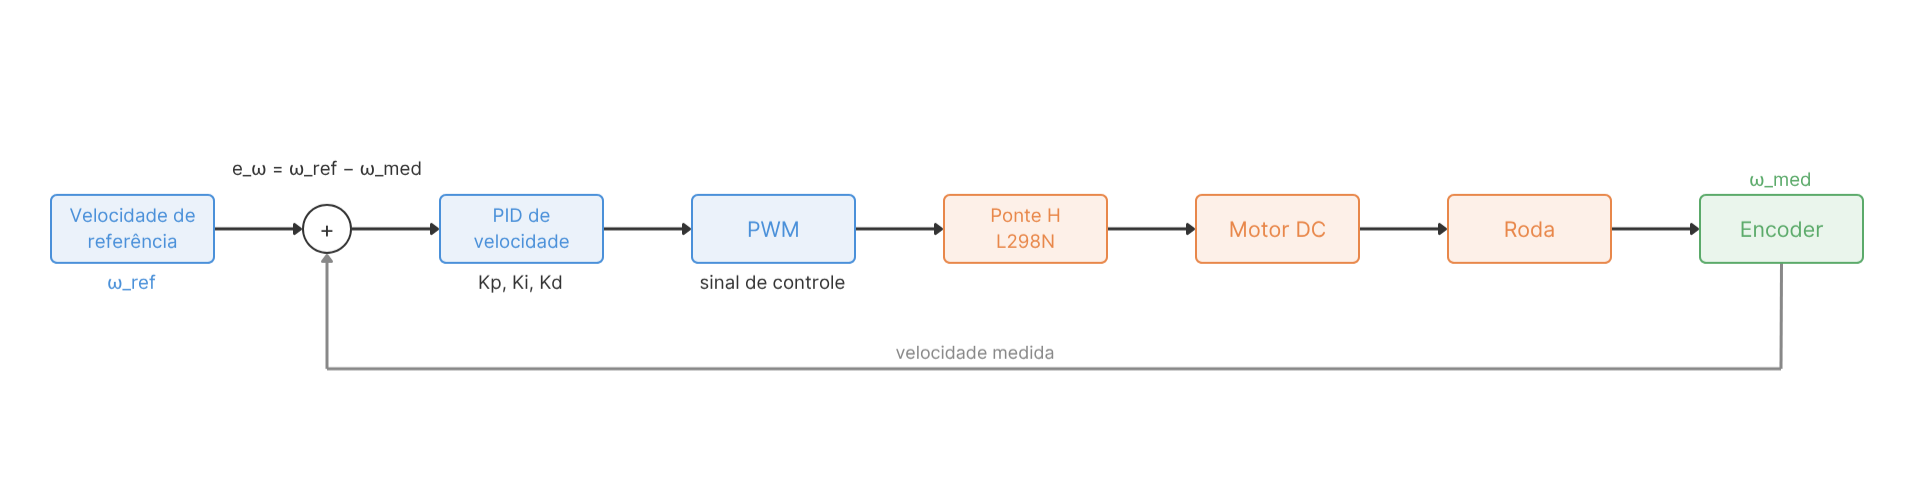
\includegraphics[width=0.9\linewidth]{imagens/Diagrama_PID_Velocidade.png}
	\caption{Diagrama simplificado da malha de controle de velocidade dos motores.}
	\label{fig:pid_velocidade}
\end{figure}

Para cada motor, o erro de velocidade é definido pela Equação~\ref{eq:erro_velocidade_pid}, como a diferença entre a velocidade angular de referência e a velocidade angular medida pelos encoders:
\begin{equation}
	e_{\omega}(t) = \omega_{\text{ref}}(t) - \omega_{\text{med}}(t)
	\label{eq:erro_velocidade_pid}
\end{equation}

em que $\omega_{\text{ref}}(t)$ representa a velocidade angular desejada e $\omega_{\text{med}}(t)$ representa a velocidade angular estimada a partir dos pulsos dos encoders. A ação de controle PID correspondente é apresentada na Equação~\ref{eq:pid_velocidade}:
\begin{equation}
	u_{\omega}(t) =
	K_{p\omega} e_{\omega}(t)
	+ K_{i\omega} \int_0^{t}e_{\omega}(\tau)d\tau
	+ K_{d\omega}\frac{de_{\omega}(t)}{dt}
	\label{eq:pid_velocidade}
\end{equation}

em que $K_{p\omega}$, $K_{i\omega}$ e $K_{d\omega}$ representam, respectivamente, os ganhos proporcional, integral e derivativo da malha de velocidade. O sinal $u_{\omega}(t)$ é convertido em um valor de PWM aplicado ao motor correspondente.

Além da malha de velocidade, o sistema utiliza uma malha de direção para corrigir desvios de orientação. Essa malha compara a orientação de referência do robô com a orientação estimada durante o movimento, produzindo uma correção angular que é distribuída entre os lados esquerdo e direito. A Figura~\ref{fig:pid_direcao} apresenta o diagrama simplificado dessa malha.

\begin{figure}[ht]
	\centering
	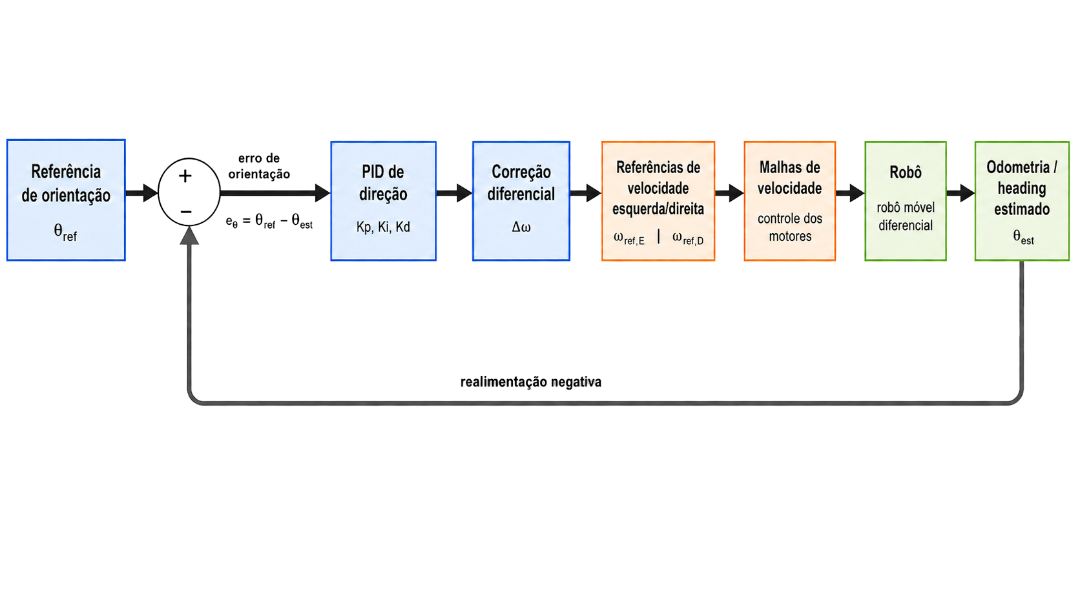
\includegraphics[width=0.95\linewidth]{imagens/Diagrama_PID_orientacao.png}
	\caption{Diagrama simplificado da malha de controle de direção do robô.}
	\label{fig:pid_direcao}
\end{figure}

O erro angular é calculado pela Equação~\ref{eq:erro_direcao_pid_bruto}, a partir da diferença entre a orientação desejada e a orientação estimada do robô:
\begin{equation}
	e_{\theta}(t) = \theta_{\text{ref}}(t) - \theta_{\text{med}}(t)
	\label{eq:erro_direcao_pid_bruto}
\end{equation}

Como a orientação é uma grandeza angular, esse erro deve ser normalizado para evitar ambiguidades entre ângulos equivalentes. O erro efetivamente utilizado pelo controlador é definido na Equação~\ref{eq:erro_direcao_pid}:
\begin{equation}
	e_{\theta}^{*}(t) =
	\mathrm{norm}\left(\theta_{\text{ref}}(t) - \theta_{\text{med}}(t)\right)
	\label{eq:erro_direcao_pid}
\end{equation}
em que $\mathrm{norm}(\cdot)$ representa a normalização do erro angular para o intervalo $[-\pi,\pi]$. A ação de controle da malha de direção é definida pela Equação~\ref{eq:pid_direcao}:
\begin{equation}
	u_{\theta}(t) =
	K_{p\theta} e_{\theta}^{*}(t)
	+ K_{i\theta} \int_0^{t}e_{\theta}^{*}(\tau)d\tau
	+ K_{d\theta}\frac{de_{\theta}^{*}(t)}{dt}
	\label{eq:pid_direcao}
\end{equation}
em que $K_{p\theta}$, $K_{i\theta}$ e $K_{d\theta}$ representam os ganhos proporcional, integral e derivativo da malha de direção. O termo $u_{\theta}(t)$ corresponde à correção angular aplicada ao movimento do robô.

Durante deslocamentos lineares, a correção angular é combinada com a velocidade base definida para o movimento. As velocidades de referência dos lados direito e esquerdo são expressas pelas Equações~\ref{eq:ref_roda_direita} e~\ref{eq:ref_roda_esquerda}:
\begin{equation}
	\omega_{\text{ref},R}(t) = \omega_{\text{ref}}(t) + u_{\theta}(t)
	\label{eq:ref_roda_direita}
\end{equation}
\begin{equation}
	\omega_{\text{ref},L}(t) = \omega_{\text{ref}}(t) - u_{\theta}(t)
	\label{eq:ref_roda_esquerda}
\end{equation}
em que $\omega_{\text{ref},R}(t)$ e $\omega_{\text{ref},L}(t)$ representam as velocidades angulares de referência para os lados direito e esquerdo, respectivamente, e $\omega_{\text{ref}}(t)$ representa a velocidade angular base do movimento. Assim, caso o robô apresente desvio de orientação, a velocidade de um lado é aumentada enquanto a do outro é reduzida, produzindo uma correção diferencial da trajetória.

Durante curvas ou manobras de rotação sobre o próprio eixo, as referências de velocidade são definidas com sinais opostos, conforme as Equações~\ref{eq:ref_roda_direita_rotacao} e~\ref{eq:ref_roda_esquerda_rotacao}:
\begin{equation}
	\omega_{\text{ref},R}(t) = +u_{\theta}(t)
	\label{eq:ref_roda_direita_rotacao}
\end{equation}

\begin{equation}
	\omega_{\text{ref},L}(t) = -u_{\theta}(t)
	\label{eq:ref_roda_esquerda_rotacao}
\end{equation}

Essa configuração permite que os lados esquerdo e direito girem em sentidos opostos, produzindo a rotação do robô em torno do próprio eixo. Na versão atual do sistema, a variação dos encoders é utilizada como critério principal de parada da rotação, com uma constante de calibração denominada \texttt{TURN\_ENCODER\_SCALE}. Essa constante foi introduzida para ajustar a relação entre a rotação estimada pelos encoders e a rotação efetivamente observada no robô durante os testes práticos.

A adoção dos encoders como referência principal para controle de rotação ocorreu após ensaios indicarem que o magnetômetro QMC5883L sofre interferências significativas durante o acionamento dos motores. Por esse motivo, o QMC5883L foi mantido como referência auxiliar de orientação, enquanto o controle direto das rotações passou a ser baseado majoritariamente na odometria dos encoders e nos critérios de validação implementados no sistema.

Dessa forma, a malha de direção atua em nível superior, definindo a correção angular necessária para manter ou alterar a orientação do robô, enquanto a malha de velocidade atua em nível inferior, ajustando o PWM dos motores para que as velocidades de referência sejam alcançadas. Essa organização em duas malhas facilita a calibração do sistema, permite compensar diferenças entre os motores e melhora a previsibilidade da movimentação do robô durante a navegação em grid.

\subsection{Sensoriamento e Mapeamento do Ambiente}

O sensor de distância VL53L0X foi incorporado ao sistema com o objetivo inicial de fornecer medições frontais de distância durante o deslocamento do robô, de modo que essas informações pudessem ser utilizadas tanto para a identificação de obstáculos quanto para a atualização de uma matriz de ocupação (\textit{grid map}). Nesse modelo, o ambiente é representado de forma discretizada, e cada célula da matriz pode assumir estados como livre, ocupada ou desconhecida, conforme as informações obtidas durante a navegação.

Entretanto, ao longo do desenvolvimento do protótipo, a estratégia de mapeamento completo em tempo real precisou ser simplificada devido a limitações práticas encontradas durante a integração mecânica e eletrônica do sistema. Assim, na versão implementada e validada experimentalmente, o robô passou a operar a partir de um mapa previamente fornecido, enquanto o sensor VL53L0X foi utilizado principalmente como mecanismo de detecção de obstáculos à frente do robô. Dessa forma, o sensor não foi utilizado para construir integralmente o mapa do ambiente durante a execução, mas sim como uma camada reativa de segurança associada à navegação em grid.

Essa decisão permitiu manter a lógica de planejamento de rotas baseada no mapa discreto, ao mesmo tempo em que o sistema continuou capaz de reagir a obstáculos não previstos na representação inicial. Durante a movimentação entre células, as leituras do VL53L0X são avaliadas para verificar se há algum objeto no caminho imediato do robô. Caso uma distância inferior ao limite definido seja detectada, o sistema interrompe ou aborta a movimentação, evitando a colisão e registrando a ocorrência como obstáculo identificado durante a navegação.

Durante a etapa de prototipagem, o sensor VL53L0X permaneceu em uma condição de montagem provisória, em razão das limitações mecânicas da estrutura utilizada e da fragilidade das conexões por jumpers. A ausência de um suporte rígido e alinhado à região frontal do robô dificultou o uso confiável do sensor para atualização contínua do mapa, pois pequenas variações de posicionamento poderiam alterar a direção do feixe de medição e comprometer a interpretação espacial das leituras. Por esse motivo, a validação concentrou-se na comunicação com o ESP32, na obtenção das medições de distância e na integração dessas informações à lógica de detecção de obstáculos.

Portanto, no escopo final deste trabalho, o VL53L0X atua como sensor de proximidade frontal para detecção de obstáculos, e não como sensor principal de mapeamento autônomo do ambiente. O mapeamento em grid permanece como estrutura de representação espacial e planejamento de rotas, porém o mapa utilizado nos testes é fornecido previamente ao sistema. Essa distinção é importante, pois separa a função de planejamento global, baseada no mapa conhecido, da função de reação local, baseada nas leituras do sensor de distância.

Em uma versão futura do protótipo, recomenda-se reposicionar e fixar o VL53L0X na região frontal do robô com suporte mecânico adequado, garantindo alinhamento estável com a direção de deslocamento. Com uma montagem mais rígida e calibrada, as medições do sensor poderiam ser utilizadas não apenas para detecção de obstáculos, mas também para atualização dinâmica do mapa de ocupação, aproximando o sistema da proposta inicial de automapeamento do ambiente.

\subsection{Planejamento de Rota com Algoritmo A*}

Com base na matriz de ocupação gerada, o planejamento de caminho entre a posição atual e o destino desejado é realizado por meio do algoritmo A* (\textit{A-star}). Esse algoritmo é amplamente utilizado em sistemas robóticos por combinar eficiência e precisão, realizando uma busca heurística que minimiza o custo total do caminho considerando a distância percorrida e a distância estimada até o objetivo.

O resultado do algoritmo é uma sequência de coordenadas representando a trajetória ideal, a qual é traduzida em comandos de movimento (frente, curva à direita, curva à esquerda, etc.) e enviada ao sistema de controle de baixo nível.

A Figura~\ref{fig:a_star_path} ilustra um exemplo visual da aplicação do algoritmo A* sobre uma matriz de ocupação, destacando um trajeto seguro entre o ponto de origem e o destino. Embora essa figura não represente o algoritmo efetivamente utilizado pelo robô, ela ajuda a visualizar o princípio de planejamento de caminhos adotado neste trabalho.

\begin{figure}[ht]
	\centering
	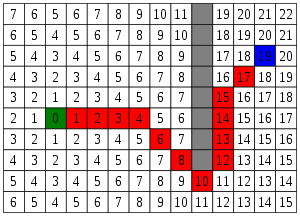
\includegraphics[width=0.5\linewidth]{imagens/a_star_example.png}
	\caption{Exemplo de caminho traçado pelo algoritmo A* sobre um mapa de ocupação.}
	\label{fig:a_star_path}
	\vspace{0.2em}
	\small\textit{Fonte: \href{https://medium.com/@nicholas.w.swift/easy-a-star-pathfinding-7e6689c7f7b2}{@nicholas.w.swift at Medium.com}}
\end{figure}

Visando a economia de bateria e a eficiência operacional, o sistema de navegação é projetado para seguir a rota planejada de forma otimizada, evitando manobras desnecessárias e reduzindo o tempo total de deslocamento. Nesse sentido, as curvas são penalizadas ao máximo, pois exigem maior esforço ao alterar o sentido de rotação dos motores, consomem mais energia e tendem a tornar a trajetória mais lenta.

\subsection{Execução da Navegação}

Após a definição da rota pelo algoritmo de planejamento, o caminho obtido é convertido em uma sequência de comandos elementares de movimento. Como o ambiente é representado por uma matriz discreta, cada etapa da rota corresponde à transição entre uma célula atual e uma célula vizinha. A partir da diferença entre as coordenadas consecutivas do caminho, o sistema determina se o robô deve manter sua orientação atual, realizar uma rotação ou avançar para a próxima célula.

Na implementação desenvolvida, os principais comandos de movimentação considerados foram:

\begin{itemize}
	\item \textbf{Avançar uma célula:} desloca o robô para frente por aproximadamente uma célula do grid, correspondente a $30\,\text{cm}$. Esse comando é utilizado quando a próxima coordenada da rota está à frente da orientação atual do robô.

	\item \textbf{Virar à esquerda:} executa uma rotação do robô para o lado esquerdo, geralmente associada a uma mudança de orientação de aproximadamente $90^\circ$, dependendo da direção exigida pela próxima célula do caminho.

	\item \textbf{Virar à direita:} executa uma rotação do robô para o lado direito, também utilizada para alinhar o robô com a próxima célula da rota planejada.

	\item \textbf{Rotacionar para orientação alvo:} ajusta a pose angular do robô para uma orientação desejada antes de iniciar o deslocamento linear. Esse comando é utilizado quando a diferença entre a orientação atual e a direção da próxima célula exige uma correção angular.

	\item \textbf{Parar:} interrompe imediatamente o acionamento dos motores. Esse comando é utilizado ao final de cada deslocamento, ao término de uma rotação, em caso de obstáculo detectado ou quando ocorre o cancelamento da navegação.

	\item \textbf{Abortar navegação:} interrompe a execução da rota atual e impede a continuidade dos comandos planejados. Esse comportamento é acionado quando o sensor frontal identifica um obstáculo inesperado ou quando alguma condição de segurança impede a continuidade do movimento.
\end{itemize}

Durante a execução da navegação, o robô não realiza o percurso de forma contínua e irrestrita. Em vez disso, a trajetória é executada de maneira incremental: o robô se orienta em direção à próxima célula, avança aproximadamente $30\,\text{cm}$, interrompe o movimento, atualiza sua pose estimada e então prossegue para a próxima etapa da rota. Essa estratégia facilita a correção de orientação entre células e reduz o acúmulo de erro durante a navegação.

O controle dos deslocamentos lineares é realizado com base na odometria dos encoders, enquanto as rotações utilizam a variação estimada pelos encoders como critério principal de parada. Para compensar diferenças entre a rotação calculada e a rotação observada no protótipo, foi utilizada uma constante de calibração denominada \texttt{TURN\_ENCODER\_SCALE}. O magnetômetro QMC5883L permanece como referência auxiliar de orientação, mas não é utilizado como critério principal de parada das rotações devido às interferências observadas durante o acionamento dos motores.

Durante todo o trajeto, o sensor VL53L0X monitora a presença de obstáculos imprevistos à frente do robô. Caso um obstáculo seja detectado durante o deslocamento para a próxima célula, o sistema interrompe a locomoção e aborta a execução atual. Na implementação testada, o mapa 7x7 utilizado nos experimentos é preservado, sem sobrescrever células dinamicamente, para evitar que leituras momentâneas do sensor modifiquem a representação base do ambiente durante a calibração.

Essa estratégia caracteriza a navegação como um processo híbrido: o planejamento global define a sequência de células a ser percorrida, enquanto o controle local executa comandos de movimento e reage a obstáculos detectados durante o trajeto. Dessa forma, o robô é capaz de executar tarefas simples de deslocamento autônomo, seguindo uma rota planejada, monitorando o ambiente imediato e interrompendo sua movimentação quando uma condição de risco é identificada.

\subsection{Calibração de Giro e Rejeição de Leituras Instáveis}

Durante os testes de rotação, verificou-se que o uso exclusivo do magnetômetro para finalizar curvas não era suficientemente confiável, pois as leituras do QMC5883L apresentavam saltos significativos quando os motores e a ponte H estavam acionados. Para contornar esse problema, a lógica de giro passou a utilizar os encoders como critério principal de parada, com uma constante de calibração denominada \texttt{TURN\_ENCODER\_SCALE}. Essa constante permite ajustar a relação entre os pulsos medidos pelos encoders e o ângulo físico efetivamente executado pelo robô.

Além disso, foi incorporada uma lógica de rejeição de leituras anômalas. No caso dos encoders, saltos incompatíveis com a velocidade esperada são descartados para evitar que um pulso espúrio encerre uma curva prematuramente. No caso do QMC5883L, leituras com inovação angular excessiva são ignoradas pelo estimador de posição, impedindo que interferências magnéticas atualizem de forma indevida a orientação do robô.

% # TODO: IMAGEM - Inserir gráfico ou captura de log mostrando a calibração de giro por encoder, incluindo raw, scaled e TURN_ENCODER_SCALE. Sugestão de arquivo: imagens/log_turn_encoder_scale.png


\section{Interface Web e Sistema de Arquivos Flash}

A interface web desenvolvida para o sistema permite o monitoramento e controle remoto do robô por meio de um navegador padrão, sem a necessidade de softwares adicionais. Esta interface é hospedada diretamente no microcontrolador ESP32, garantindo autonomia e independência de conexões externas. Os arquivos estáticos, compostos por páginas HTML, folhas de estilo CSS e scripts JavaScript, são armazenados e carregados utilizando o sistema de arquivos SPIFFS, otimizado para dispositivos embarcados com memória limitada.

Para viabilizar a comunicação bidirecional em tempo real entre a interface e o robô, emprega-se o protocolo WebSocket. Esse protocolo possibilita a atualização contínua do status dos sensores, bem como o envio imediato de comandos de movimentação e controle, garantindo uma resposta rápida e eficiente. O uso de WebSocket também minimiza a sobrecarga de comunicação e otimiza o consumo de recursos do ESP32, assegurando estabilidade e desempenho adequados para a aplicação.

% \begin{figure}[ht!]
% 	\centering
% 	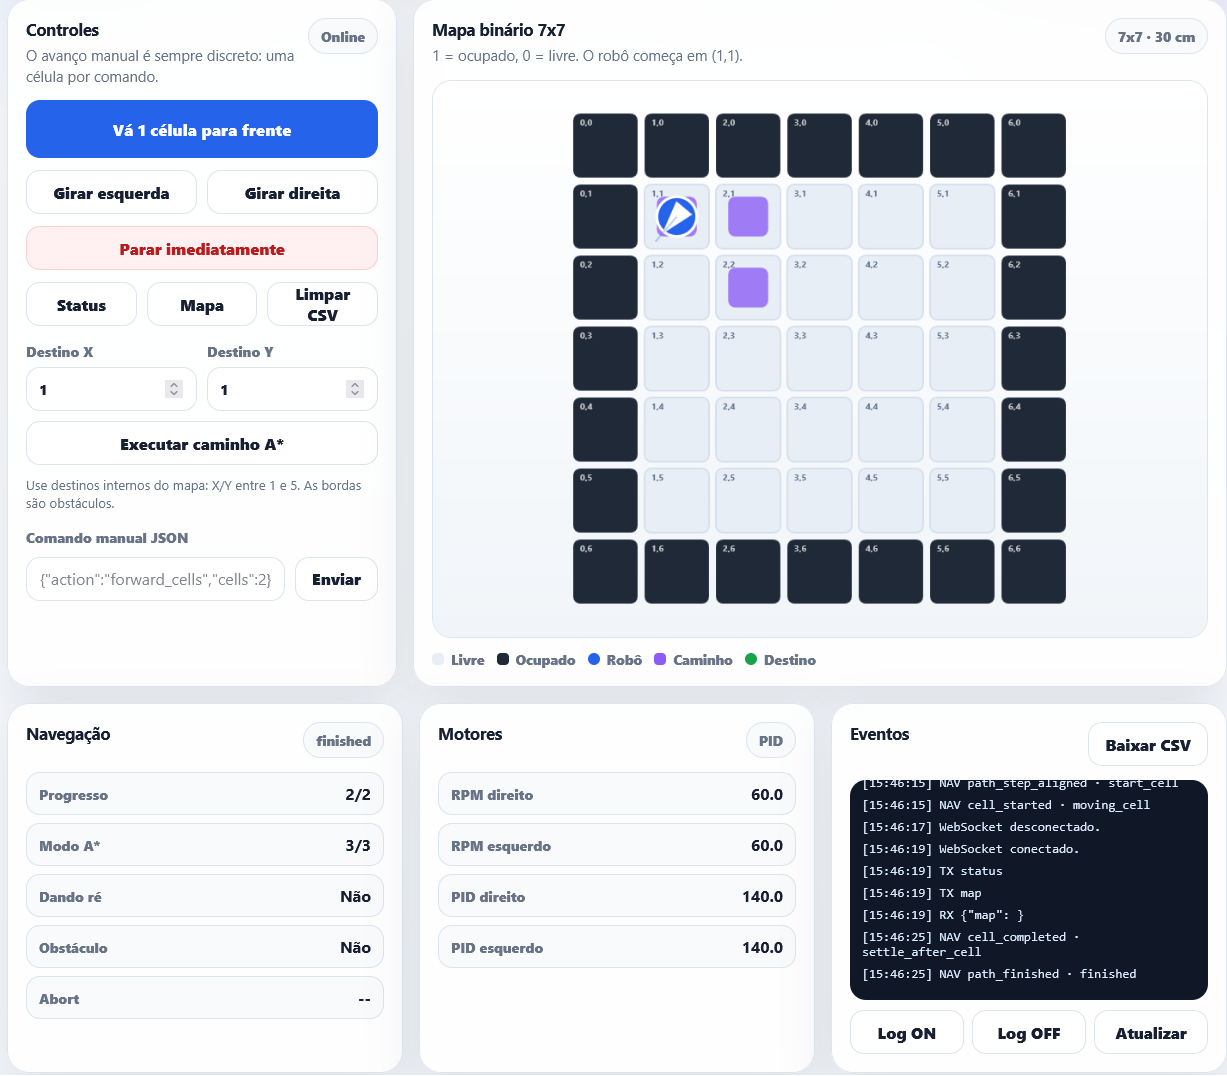
\includegraphics[width=0.9\linewidth]{imagens/Interface_Controle.png}
% 	\caption{Interface web principal do robô, exibindo o mapa de ocupação, botões de controle e telemetria em tempo real.}
% 	\label{fig:interface_web_principal}
% \end{figure}
% % # TODO: IMAGEM - Inserir screenshot da tela de monitor/logs mostrando telemetria de encoders, QMC5883L, VL53L0X e estado da navegação. Sugestão de arquivo: imagens/interface_monitor_logs.png

\section{Descrição dos Testes} \label{sec:descricao_testes}

Para avaliar o funcionamento do sistema desenvolvido, foram definidos testes experimentais com o objetivo de verificar o comportamento do robô em tarefas básicas de navegação em grid, deslocamento linear, rotação, localização estimada e detecção de obstáculos. Os testes foram planejados considerando o mapa discreto utilizado no projeto, composto por células de $30\,\text{cm} \times 30\,\text{cm}$, no qual a posição do robô é representada por coordenadas $(x,\ y)$. Para testes, foi feito o uso de fitas adesivas para demarcar as células no chão, criando um ambiente controlado para a validação dos movimentos e da lógica de navegação. A Figura~\ref{fig:teste_grid} apresenta a configuração do ambiente de teste, evidenciando as células do grid demarcadas por fitas adesivas.

\begin{figure}[ht!]
	\centering
	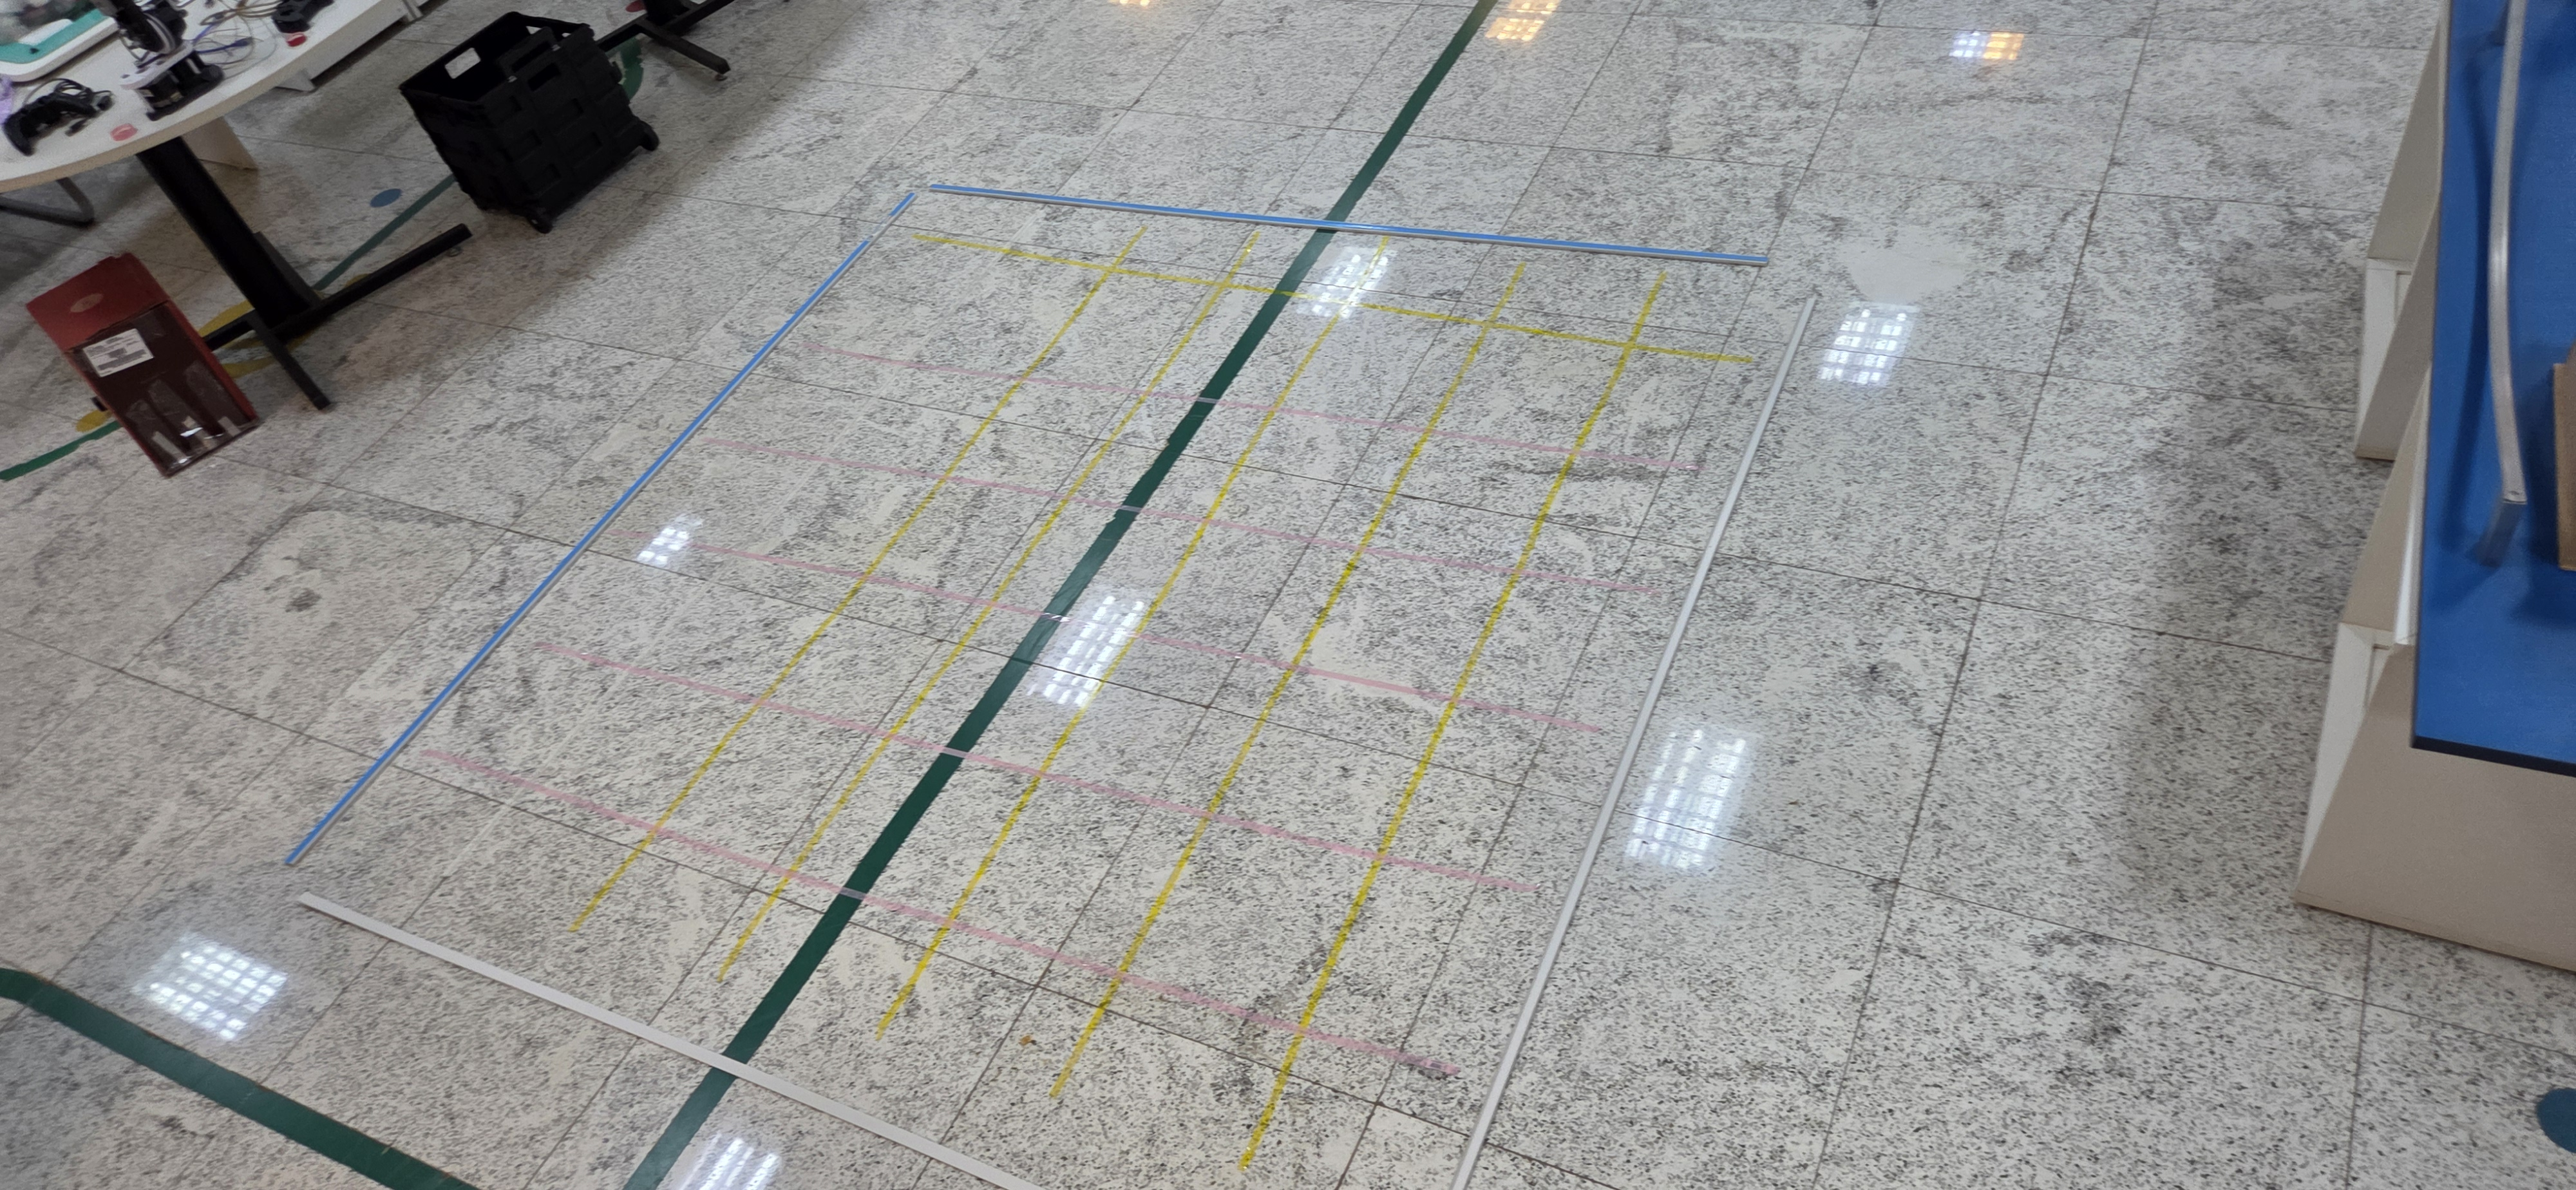
\includegraphics[width=0.9\linewidth]{imagens/Teste_Grid.jpg}
	\caption{Configuração do ambiente de teste, com demarcação das células do grid utilizando fitas adesivas.}
	\label{fig:teste_grid}
\end{figure}

Em todos os testes, considerou-se que o robô inicia sua operação em uma célula conhecida do grid, com orientação inicial definida. A célula inicial adotada, $(1,1)$, corresponde à origem operacional do sistema de coordenadas global utilizado nos ensaios, enquanto a origem matricial $(0,0)$ permanece localizada no canto superior esquerdo do mapa. A execução foi acompanhada por meio da interface web embarcada, dos registros de telemetria e dos logs gerados pelo sistema. As métricas utilizadas para avaliação foram: número de células concluídas, distância estimada por célula, erro de deslocamento em relação aos $30\,\text{cm}$ nominais, comportamento das rotações, caminho calculado pelo A* modificado, quantidade de transições e curvas da rota, detecção de obstáculos e interrupção segura da navegação.

\subsection*{Teste 1 - Deslocamento linear entre células}
\label{sec:teste_deslocamento_linear}

O primeiro teste teve como objetivo avaliar a capacidade do robô de executar deslocamentos lineares entre células consecutivas do grid. Nesse ensaio, o robô parte de uma posição inicial conhecida e deve avançar por uma sequência de células livres, mantendo a orientação e interrompendo o movimento ao final de cada célula.

Para esse teste, definiu-se como posição inicial a coordenada $(1,\ 1)$ e como posição final esperada a coordenada $(1,\ 5)$, considerando deslocamentos sucessivos no eixo vertical do mapa. Dessa forma, o robô deve executar quatro deslocamentos lineares consecutivos, cada um correspondente a uma célula de aproximadamente $30\,\text{cm}$.

As métricas observadas nesse teste foram:

\begin{itemize}
	\item \textbf{Número de células concluídas:} quantidade de células percorridas com sucesso até a posição final ou até uma interrupção da navegação;
	\item \textbf{Distância estimada por célula:} valor calculado pela odometria ao final de cada deslocamento, comparado com a referência de $30\,\text{cm}$;
	\item \textbf{Erro de deslocamento por célula:} diferença entre a distância estimada e a distância nominal da célula;
	\item \textbf{Manutenção da orientação:} avaliação do desvio angular acumulado durante o deslocamento linear.
\end{itemize}

Esse teste permite verificar se o sistema de odometria por encoders é capaz de estimar deslocamentos compatíveis com o tamanho das células do grid, além de avaliar se a lógica de navegação incremental consegue avançar célula por célula sem executar o percurso de forma contínua e descontrolada.

\subsection*{Teste 2 - Navegação com mudança de direção}
\label{sec:teste_mudanca_direcao}

O segundo teste teve como objetivo avaliar a execução de uma rota que exige mudança de orientação durante o percurso. Diferentemente do teste anterior, neste ensaio o robô deve combinar deslocamentos lineares e comandos de rotação, verificando a integração entre o planejamento de rota, o controle de direção e o controle de velocidade dos motores.

Para esse teste, definiu-se como posição inicial a coordenada $(1,\ 1)$ e como posição final a coordenada $(3,\ 3)$, não alinhada diretamente com a orientação inicial do robô. Nesse cenário, a rota planejada exige deslocamentos lineares e ao menos uma mudança de orientação antes de alcançar a posição final.

As métricas observadas nesse teste foram:

\begin{itemize}
	\item \textbf{Conclusão da rota planejada:} verificação se o robô atingiu a coordenada final prevista pelo planejador;
	\item \textbf{Quantidade de rotações executadas:} número de comandos de giro realizados durante a rota;
	\item \textbf{Erro angular interno após rotação:} diferença entre o ângulo alvo e o ângulo estimado pelos encoders após a manobra;
	\item \textbf{Estabilidade do controle:} observação de travamentos, oscilações e correções excessivas durante a execução;
	\item \textbf{Comportamento da constante \texttt{TURN\_ENCODER\_SCALE}:} verificação se a calibração aplicada à rotação por encoders produz giros compatíveis com os ângulos esperados.
\end{itemize}

Esse teste permite avaliar o funcionamento conjunto das malhas de controle de velocidade e direção, bem como a capacidade do robô de converter uma rota planejada em comandos elementares de movimento, como avançar uma célula, virar à esquerda, virar à direita e parar ao final de cada etapa.

\subsection*{Teste 3 - Detecção de obstáculo durante a navegação}
\label{sec:teste_obstaculo}

O terceiro teste avaliou a reação do sistema diante de um obstáculo frontal durante a navegação. O robô foi colocado em uma célula conhecida do grid e recebeu um destino que exigia deslocamento por células livres. Após o início do movimento, um objeto foi posicionado à frente do sensor VL53L0X, dentro da trajetória imediata do robô, para verificar se a leitura de distância provocava a interrupção dos motores e o abortamento da execução atual.

As métricas observadas nesse teste foram:

\begin{itemize}
	\item \textbf{Detecção do obstáculo:} verificação se o sensor VL53L0X identificou a presença do objeto à frente do robô;
	\item \textbf{Interrupção segura do movimento:} análise se o robô interrompeu os motores após a detecção;
	\item \textbf{Interrupção da execução atual:} verificação se a navegação foi abortada após a detecção;
	\item \textbf{Preservação do mapa base:} verificação se o mapa 7x7 permaneceu inalterado;
	\item \textbf{Registro do evento em log:} confirmação de que o sistema registrou a detecção e o abortamento.
\end{itemize}

Esse teste permite avaliar a função reativa do sensor VL53L0X no sistema final. Embora o objetivo inicial do projeto envolvesse o uso do sensor para mapeamento dinâmico, na implementação validada experimentalmente ele foi empregado principalmente como mecanismo de detecção de obstáculos, atuando como uma camada de segurança durante a navegação.

\subsection*{Teste 4 - Navegação em grade com A* modificado}
\label{sec:teste_a_star_modificado}

O teste de navegação em grade teve como objetivo avaliar o funcionamento integrado do sistema de planejamento de rotas e execução de movimentos no mapa discreto utilizado pelo robô. Nesse ensaio, o robô parte de uma posição inicial conhecida, localizada no canto superior esquerdo da área navegável do mapa, e deve atingir uma posição final definida pelo usuário por meio da interface web.

Para esse teste, foi utilizado o mapa discreto 7x7 apresentado anteriormente, com bordas ocupadas e células internas livres ou bloqueadas conforme a configuração experimental. A rota entre a origem e o destino é calculada por uma versão modificada do algoritmo A*. Além do custo associado ao deslocamento entre células vizinhas, o planejador aplica uma penalização adicional para mudanças de direção, reduzindo a tendência de gerar trajetórias com muitas curvas consecutivas.

Essa modificação foi adotada porque, no protótipo físico, cada mudança de direção exige uma manobra de rotação, seguida de realinhamento e deslocamento linear. Assim, trajetórias com menor número de curvas tendem a ser mais adequadas para o robô, pois reduzem o acúmulo de erro angular, diminuem o tempo de execução e simplificam o controle dos motores.

Durante a execução, o caminho planejado pelo A* modificado é convertido em uma sequência de comandos elementares, como avançar uma célula, virar à esquerda, virar à direita, rotacionar para uma orientação alvo e parar. A cada etapa, o robô atualiza sua posição estimada, verifica a conclusão do movimento e monitora a presença de obstáculos por meio do sensor VL53L0X.

As métricas observadas nesse teste foram:

\begin{itemize}
	\item \textbf{Caminho gerado pelo A*:} sequência de células calculada entre a posição inicial e a posição final;
	\item \textbf{Quantidade de células percorridas:} número de transições executadas ao longo do caminho planejado;
	\item \textbf{Quantidade de curvas planejadas:} número de mudanças de direção presentes na rota gerada;
	\item \textbf{Conclusão lógica da rota:} verificação se a sequência de células calculada alcança a coordenada final definida;
	\item \textbf{Conversão da rota em comandos:} verificação da geração de comandos de avanço e rotação correspondentes às transições da rota.
\end{itemize}

Esse teste é o mais abrangente da validação experimental, pois combina o planejamento global de rotas com a execução local dos movimentos do robô. Além disso, permite verificar se a penalização de curvas no A* produz trajetórias mais compatíveis com as limitações físicas do protótipo e com a estratégia de deslocamento célula a célula adotada no sistema.

\subsection*{Síntese das métricas de avaliação}

A Tabela~\ref{tab:metricas_testes} resume os principais testes definidos e as métricas utilizadas para avaliar o funcionamento do robô.

\begin{table}[ht]
	\centering
	\caption{Testes definidos para avaliação experimental do sistema}
	\label{tab:metricas_testes}
	\begin{tabular}{|p{3.2cm}|p{4.2cm}|p{7.2cm}|}
		\hline
		\textbf{Teste} & \textbf{Objetivo} & \textbf{Métricas avaliadas} \\
		\hline
		Deslocamento linear entre células & Verificar avanço em células consecutivas do grid & Número de células concluídas, distância estimada por célula, erro de deslocamento e manutenção da orientação \\
		\hline
		Navegação com mudança de direção & Avaliar integração entre deslocamento linear, rotação e planejamento de rota & Quantidade de rotações, erro angular interno, estabilidade do controle e comportamento do \texttt{TURN\_ENCODER\_SCALE} \\
		\hline
		Detecção de obstáculo & Verificar reação local diante de obstáculo inesperado & Detecção pelo VL53L0X, interrupção dos motores, abortamento da execução, preservação do mapa e registro em log \\
		\hline
		Navegação em grade com A* modificado & Avaliar o planejamento global e a conversão da rota em movimentos & Caminho gerado, quantidade de transições, número de curvas, alcance lógico do destino e comandos produzidos \\
		\hline
	\end{tabular}
\end{table}

Os resultados obtidos a partir desses testes são apresentados e discutidos no capítulo seguinte, permitindo verificar se o robô foi capaz de executar deslocamentos compatíveis com o tamanho das células, realizar rotações controladas, reagir a obstáculos e manter uma estimativa coerente de sua posição durante a navegação.

% TODO: IMAGEM - Inserir fotografia do ambiente de teste usado para a navegação em grade, preferencialmente com marcação física das células de aproximadamente 30 cm. Sugestão de arquivo: imagens/ambiente_teste_grid_30cm.jpg
% TODO: IMAGEM - Inserir fotografia atual do robô no ambiente de teste, com o sensor VL53L0X visível na parte frontal e os encoders/motores identificáveis. Sugestão de arquivo: imagens/prototipo_teste_frontal.jpg
% FIXME: Informar no texto final o local exato onde os testes foram executados, por exemplo laboratório, sala, bancada ou corredor, e se o piso era liso, emborrachado ou irregular.

\chapter{Resultados} \label{chap:resultados}

Este capítulo apresenta os principais resultados obtidos durante o desenvolvimento e a validação experimental do robô móvel autônomo. A análise foi organizada em três resultados principais: a montagem final do protótipo físico, a interface web desenvolvida para operação e monitoramento do sistema, e o funcionamento integrado do robô durante os testes de navegação.

O primeiro resultado corresponde à consolidação do protótipo físico, incluindo a integração entre chassi, motores, encoders, sensores, ponte H, módulo de alimentação e ESP32. Nessa etapa, são apresentadas as características construtivas do robô, suas dimensões físicas e a disposição geral dos componentes embarcados.

O segundo resultado refere-se à interface web final, utilizada para acompanhar o estado do sistema e enviar comandos ao robô. A interface reúne recursos como visualização do mapa em grade, indicação da posição estimada, comandos manuais de movimentação, seleção de destino e monitoramento de dados de telemetria. Essa parte também permite relacionar o tamanho físico do robô com as células do mapa, definidas como quadrados de $30\,\text{cm} \times 30\,\text{cm}$.

O terceiro resultado trata do funcionamento integrado do sistema, utilizando os testes definidos no capítulo de Materiais e Métodos. Nessa etapa, são avaliados o deslocamento entre células, as rotações, a detecção de obstáculos e a navegação em grade com rotas geradas pelo algoritmo A* modificado, que penaliza mudanças de direção.

Para a análise deste resultado, foram utilizados os testes definidos na Seção~\ref{sec:descricao_testes} do Capítulo~\ref{cap:materiais_metodos}, especialmente os Testes~\ref{sec:teste_deslocamento_linear}, \ref{sec:teste_mudanca_direcao}, \ref{sec:teste_obstaculo} e \ref{sec:teste_a_star_modificado}.

O objetivo deste capítulo não é apenas relatar que o protótipo foi montado, mas demonstrar quais partes do sistema apresentaram comportamento funcional, quais limitações foram observadas e quais ajustes técnicos foram necessários para tornar a navegação mais previsível. Por esse motivo, os resultados são apresentados juntamente com uma discussão técnica dos principais problemas identificados durante os ensaios.

\section{Montagem Final do Protótipo}
\label{sec:resultados_montagem_final}

A montagem final do protótipo constitui um dos resultados centrais deste trabalho, pois demonstra a integração física entre a estrutura mecânica, o sistema de alimentação, os sensores, os atuadores e o microcontrolador. A Figura~\ref{fig:resultado_robo_superior} apresenta a vista superior do robô montado, permitindo observar a distribuição dos componentes sobre o chassi e a organização geral do cabeamento.

\begin{figure}[H]
	\centering
	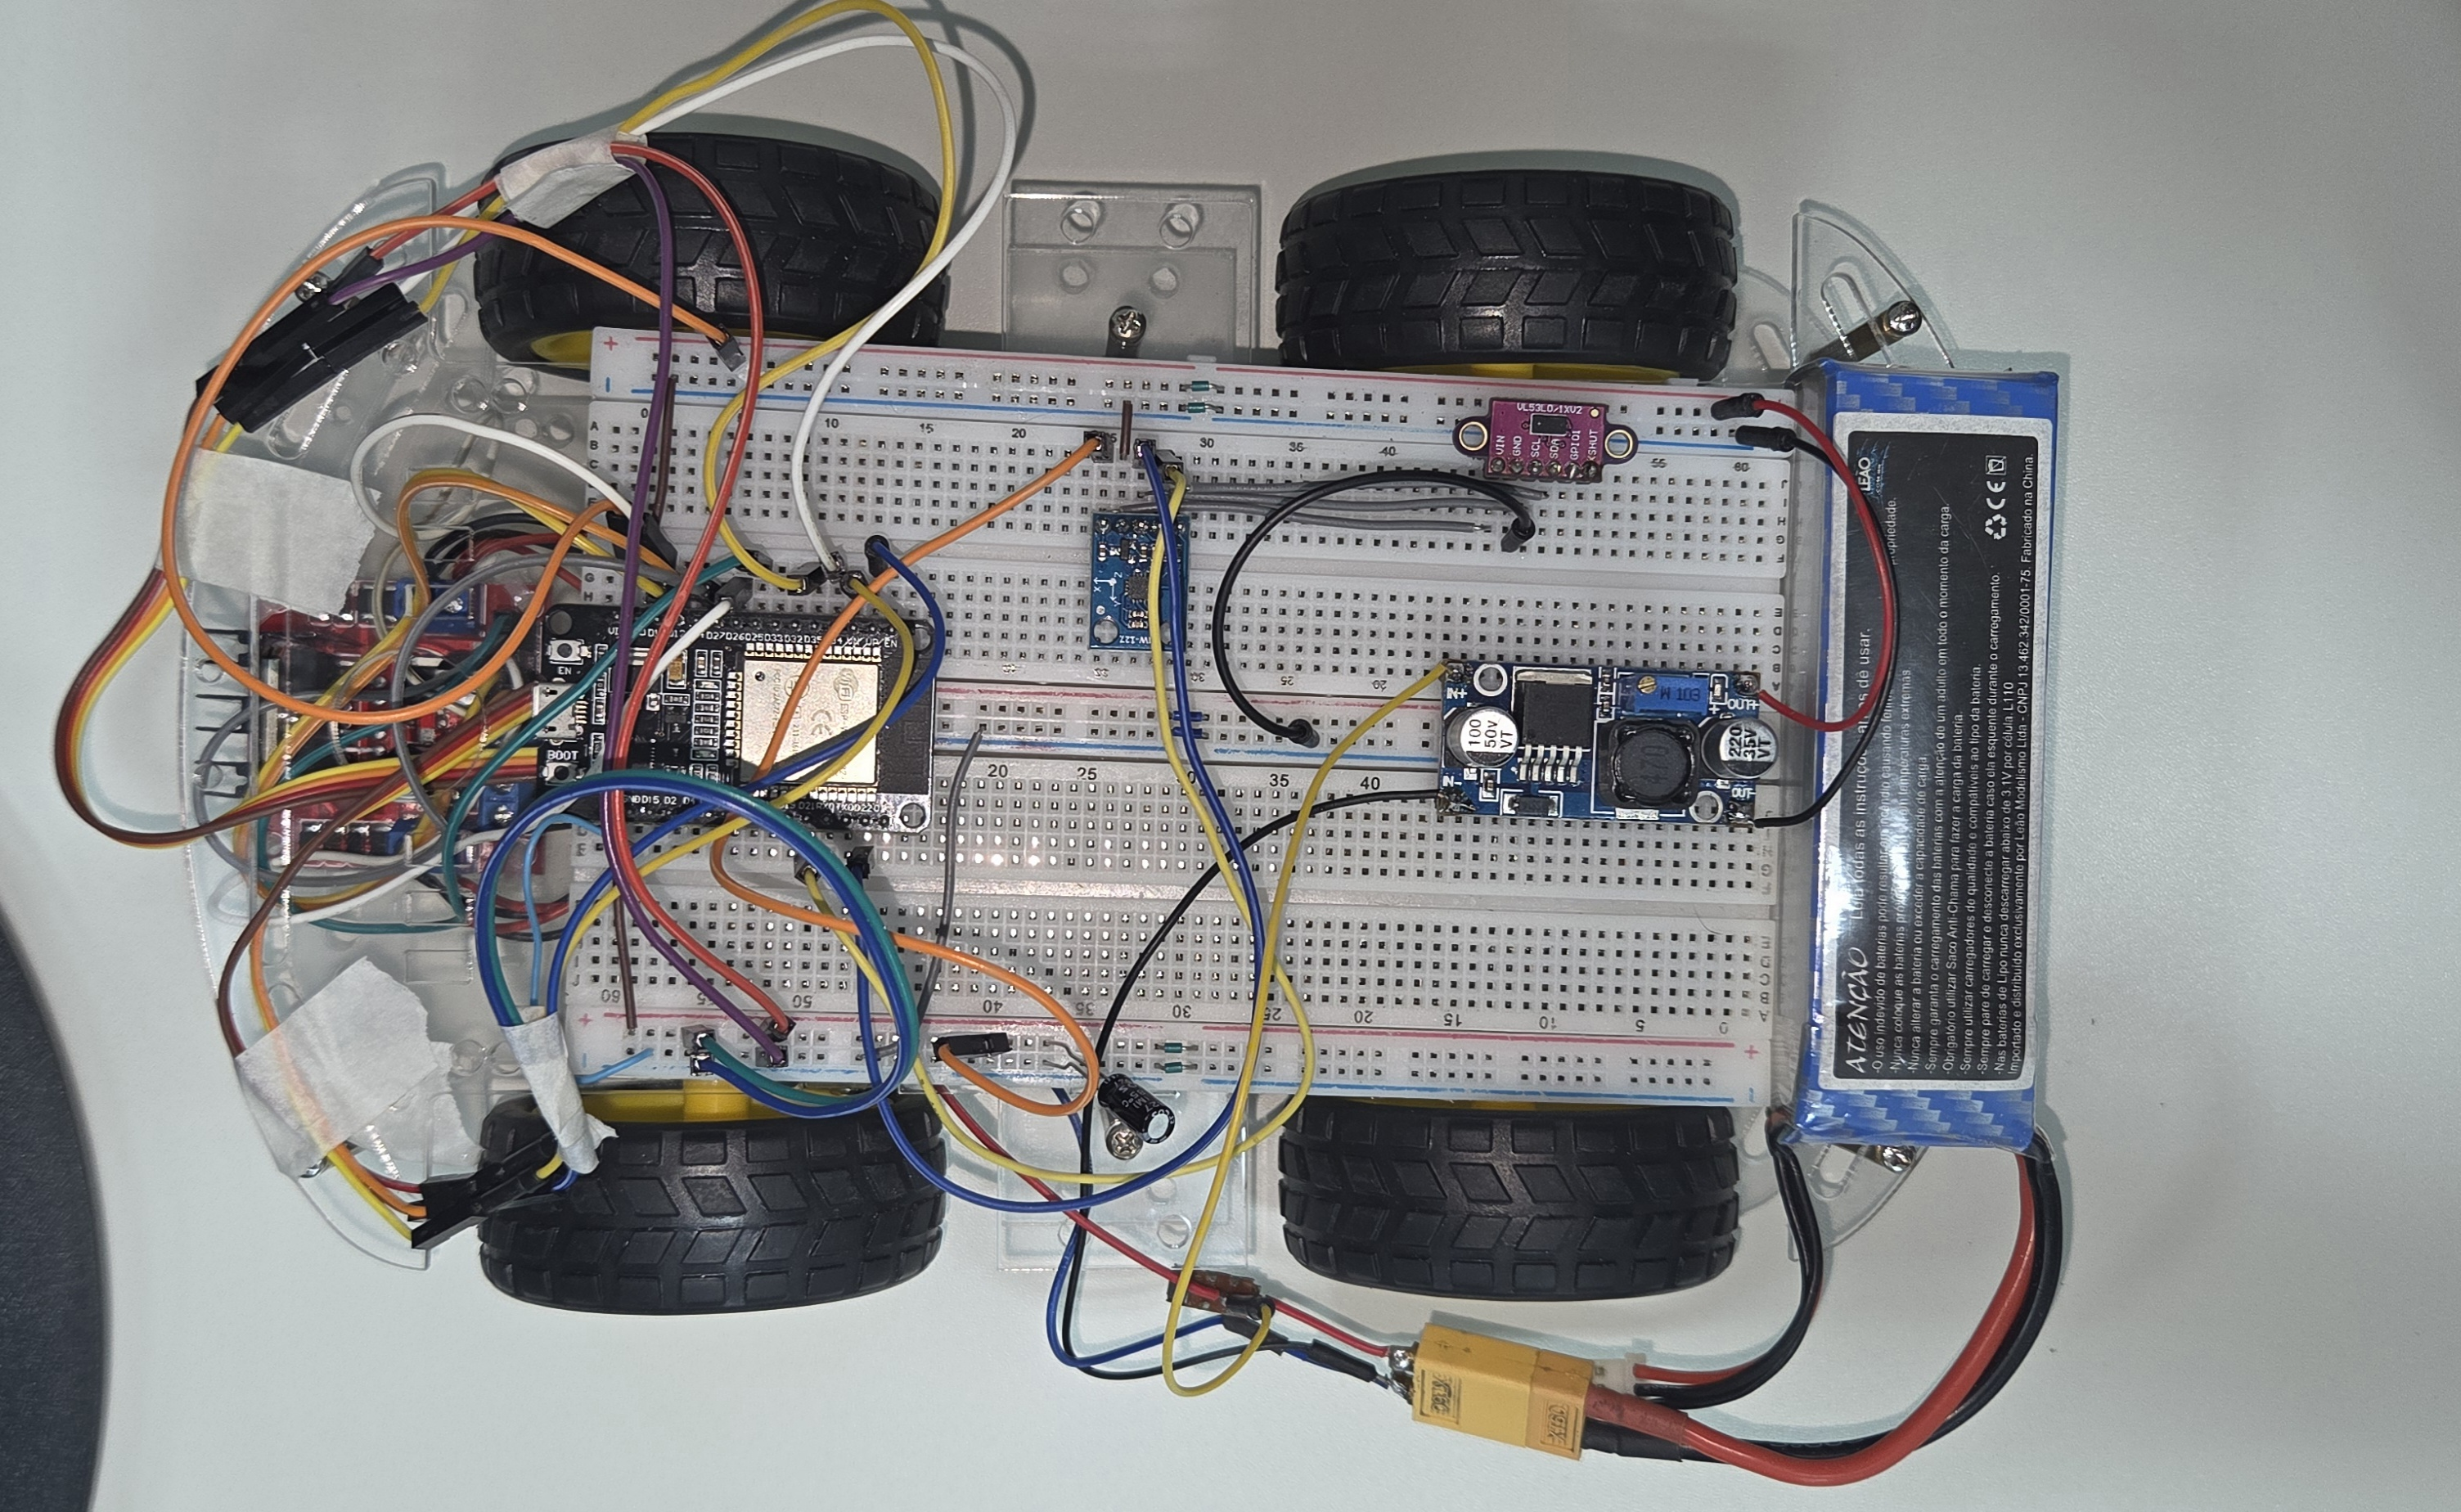
\includegraphics[width=0.75\linewidth]{imagens/Prototipo_Visao_Superior.jpg}
	\caption{Vista superior do protótipo final montado.}
	\label{fig:resultado_robo_superior}
	\vspace{0.2em}
	\small\textit{Fonte: O próprio autor.}
\end{figure}

A Figura~\ref{fig:resultado_detalhes_montagem} complementa a vista superior ao mostrar detalhes da região frontal interna e da parte traseira do protótipo. Nessas imagens, podem ser observados o posicionamento dos motores, encoders, fios, ponte H e demais módulos utilizados na montagem final.

\begin{figure}[H]
	\centering
	\begin{subfigure}[b]{0.48\linewidth}
		\centering
		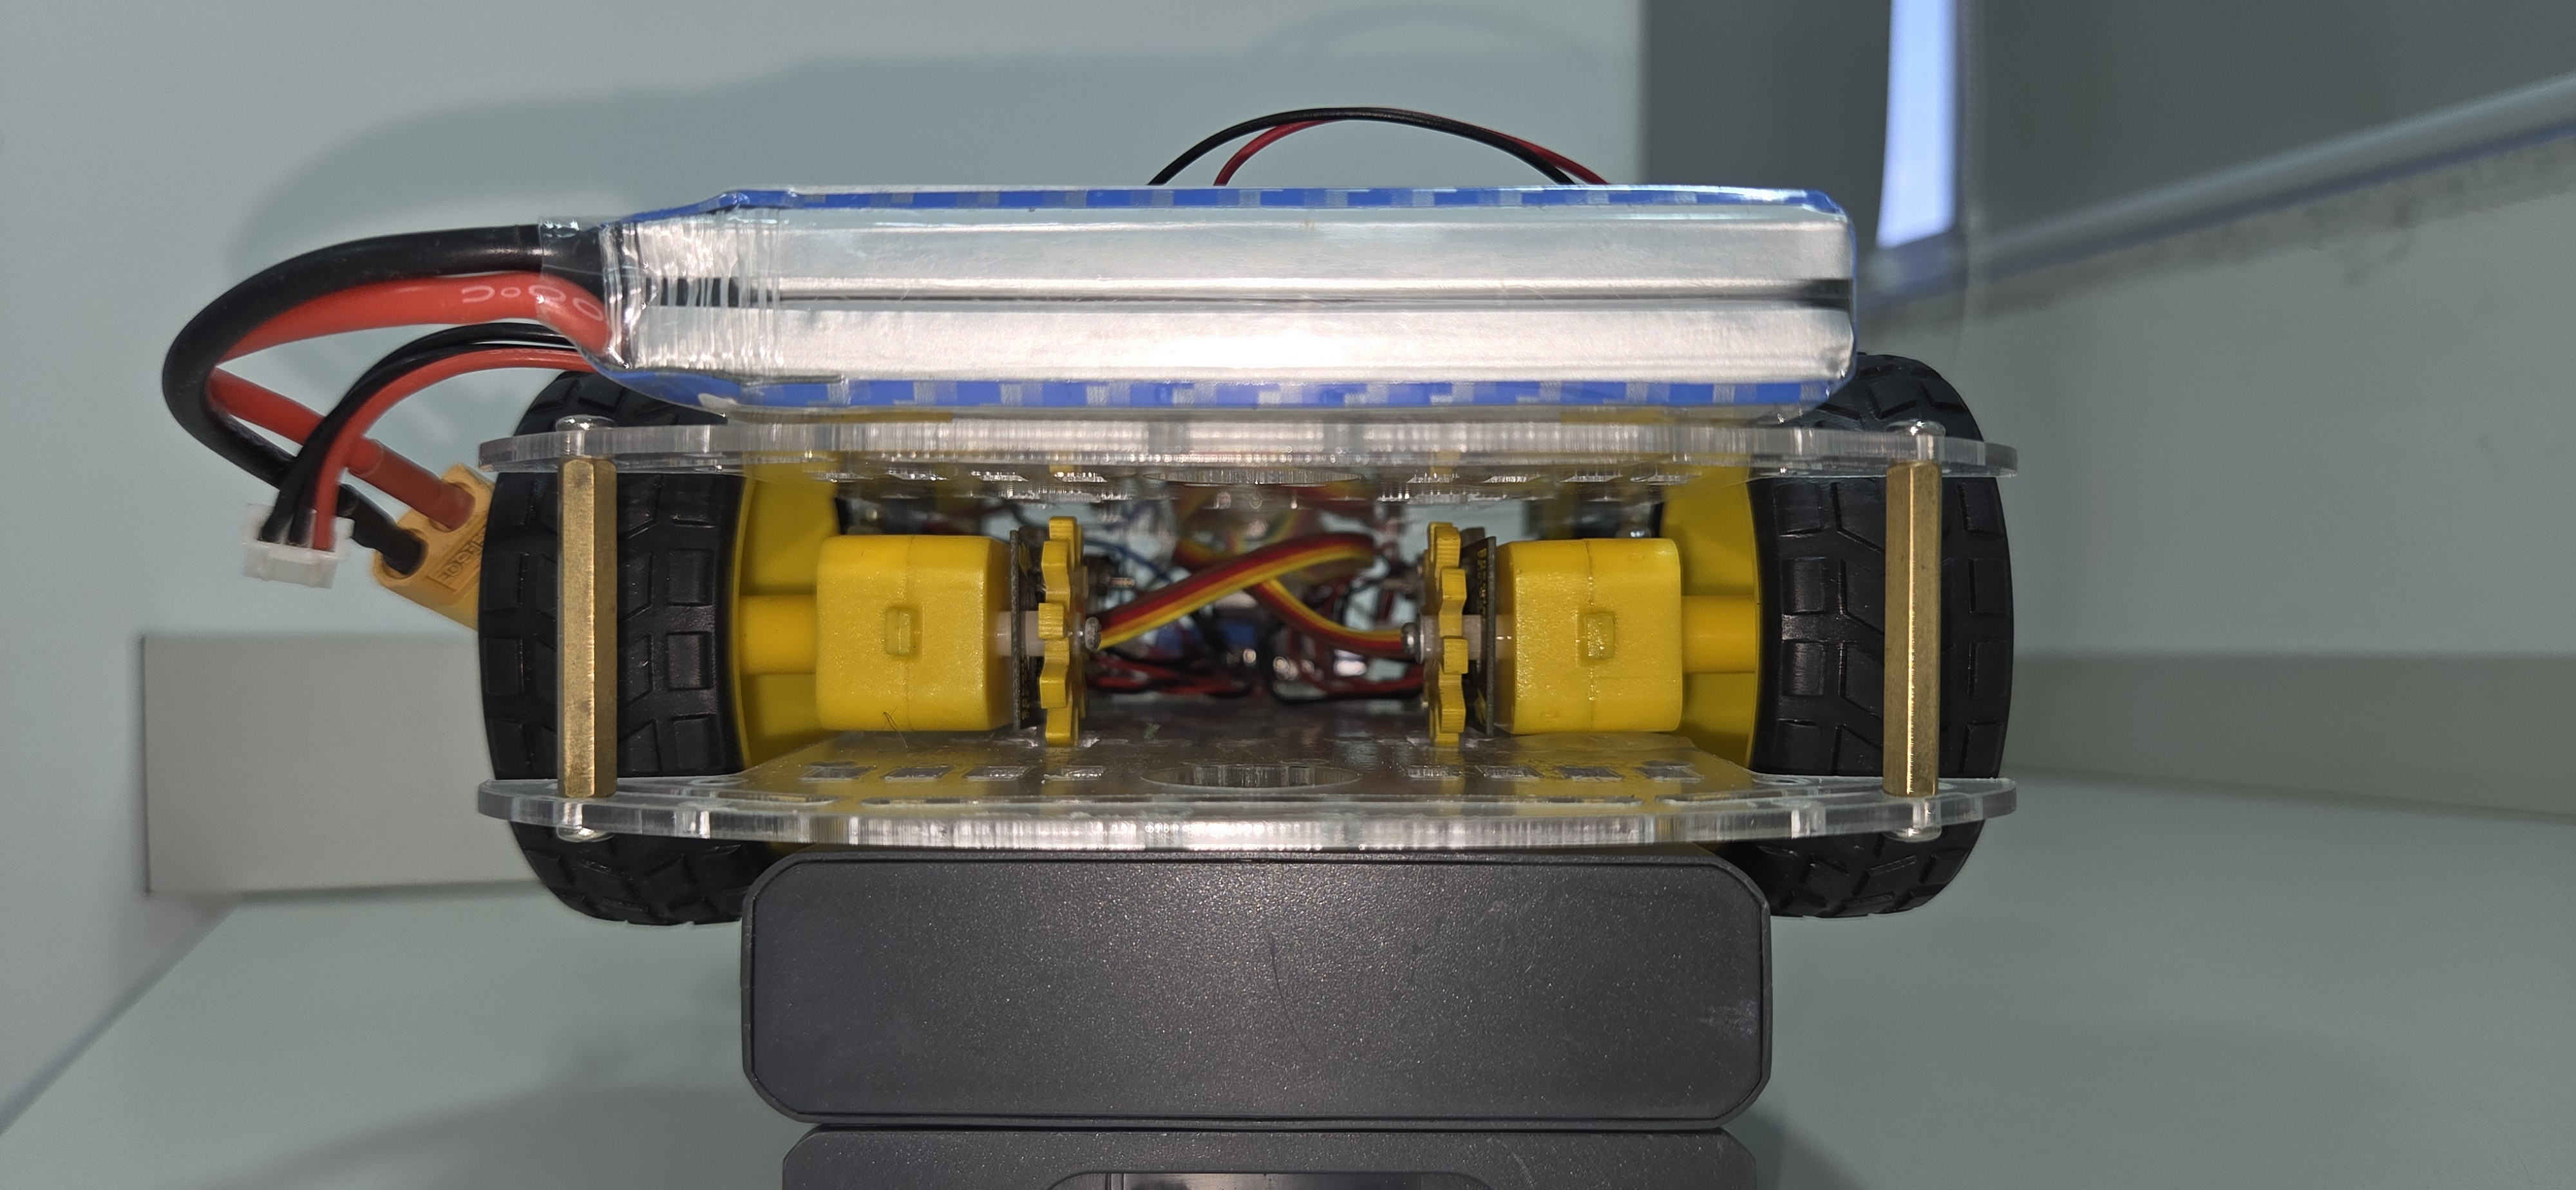
\includegraphics[width=0.9\linewidth]{imagens/Prototipo_Visao_Frontal_Interna.jpg}
		\caption{Vista frontal interna.}
	\end{subfigure}
	\hfill
	\begin{subfigure}[b]{0.48\linewidth}
		\centering
		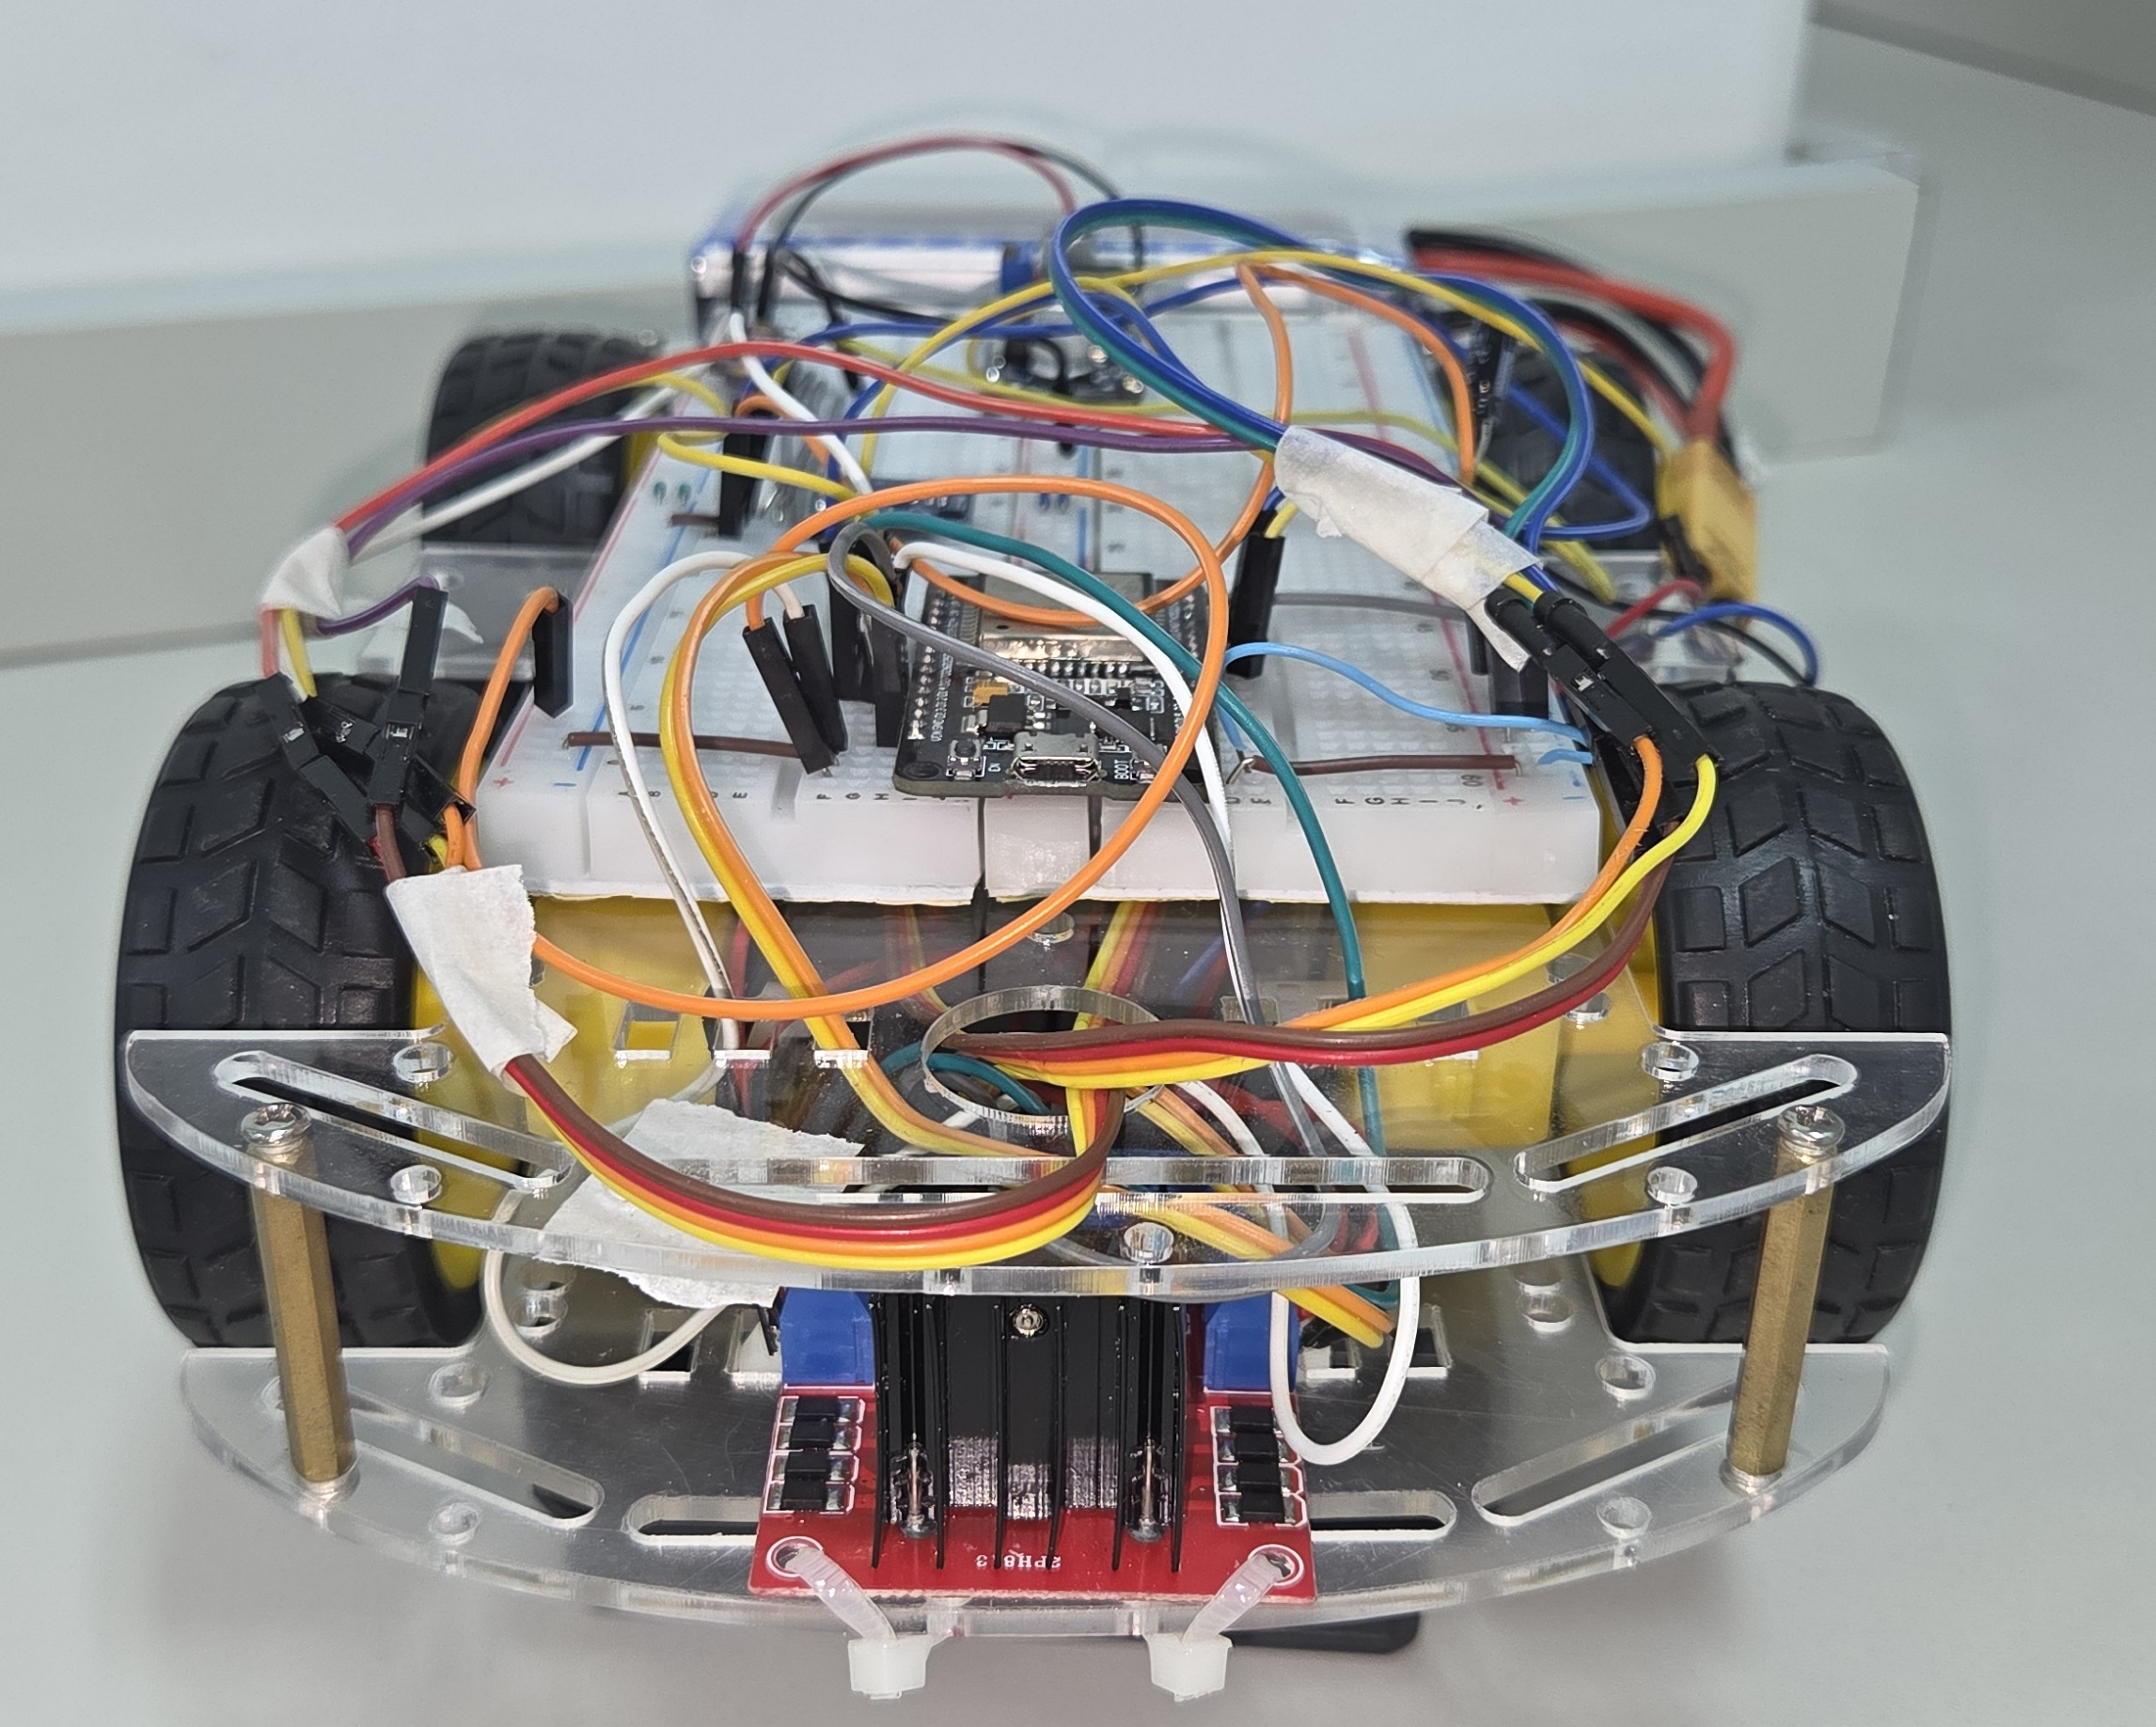
\includegraphics[width=0.9\linewidth]{imagens/Prototipo_Visao_Traseira_Superior.jpg}
		\caption{Vista traseira superior.}
	\end{subfigure}
	\caption{Detalhes da montagem final do protótipo.}
	\label{fig:resultado_detalhes_montagem}
\end{figure}

O protótipo possui aproximadamente $26\,\text{cm}$ de comprimento e $15\,\text{cm}$ de largura. Essas dimensões confirmam que sua projeção física é compatível com as células de $30\,\text{cm} \times 30\,\text{cm}$ utilizadas no ambiente experimental, restando uma margem aproximada de $4\,\text{cm}$ no sentido longitudinal e $15\,\text{cm}$ no sentido transversal quando o robô está centralizado na célula.

% FIXME: Confirmar se as dimensões finais do robô permanecem em 26 cm por 15 cm após a montagem completa.
% TODO: Informar também a altura total do protótipo, caso essa medida seja utilizada na versão final do texto.

\section{Mapa de Teste e Planejamento de Rotas}
\label{sec:resultados_mapa_planejamento}

Para os ensaios de navegação foi utilizado um mapa discreto 7x7, onde a região física pode ser encontrada na Figura \ref{fig:teste_grid}, no qual as bordas foram marcadas como células ocupadas e a região interna como área navegável. A célula inicial do robô foi definida em \((1,1)\), considerando a origem \((0,0)\) no canto superior esquerdo. Essa escolha simplifica a representação espacial e permite que os deslocamentos sejam tratados como transições discretas entre células adjacentes.

A Figura~\ref{fig:mapa-7x7-resultados} apresenta o mapa utilizado nos testes de navegação por células. Nessa representação, as células escuras indicam regiões ocupadas ou intransponíveis, enquanto as células claras representam posições livres para navegação. O robô inicia sua movimentação na célula \((1,1)\), indicada visualmente no mapa, e os destinos dos testes são definidos dentro da área livre do grid.

\begin{figure}[H]
	\centering
	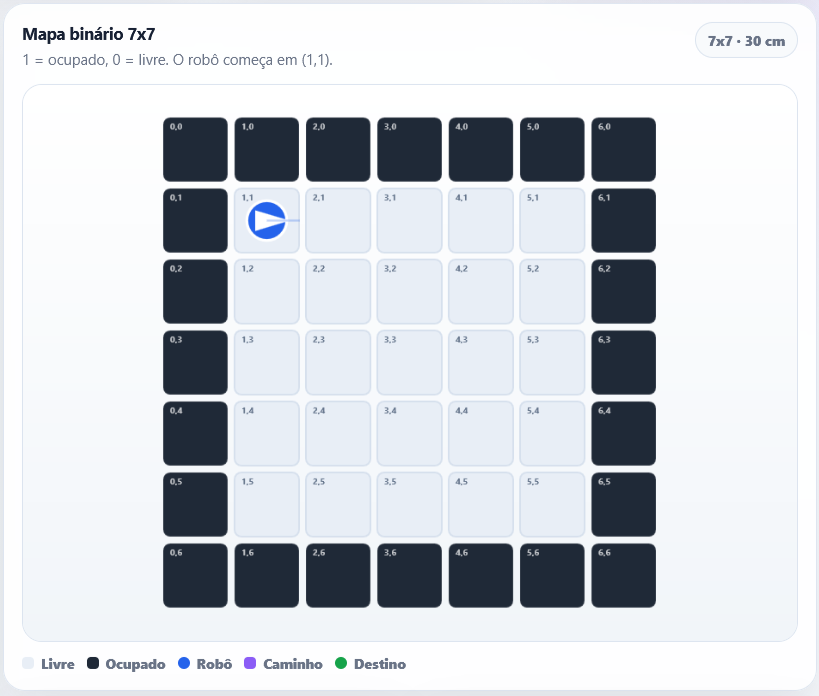
\includegraphics[width=0.65\linewidth]{imagens/mapa_utilizado_7x7.png}
	\caption{Mapa 7x7 utilizado nos testes de navegação por células.}
	\label{fig:mapa-7x7-resultados}
\end{figure}

O planejamento de rotas foi realizado por meio de uma versão modificada do algoritmo A*. O algoritmo calcula uma sequência de células entre a posição inicial e o destino definido pelo usuário, considerando as células livres e ocupadas do mapa. Além do custo de deslocamento entre células adjacentes, foi adicionada uma penalização para mudanças de direção, com o objetivo de reduzir a quantidade de curvas geradas na rota final.

Essa modificação é importante para o protótipo físico, pois cada curva exige uma manobra de rotação, seguida de realinhamento e deslocamento linear. Assim, mesmo quando existem caminhos com o mesmo comprimento em número de células, a versão modificada do A* tende a favorecer trajetórias com menor quantidade de mudanças de direção, tornando a execução mais compatível com as limitações mecânicas do robô.

De forma simplificada, o custo de uma transição entre duas células pode ser representado por:

\begin{equation}
	C = C_{\text{deslocamento}} + C_{\text{curva}}
	\label{eq:custo_astar_modificado}
\end{equation}
em que \(C_{\text{deslocamento}}\) representa o custo de avançar para uma célula vizinha e \(C_{\text{curva}}\) representa uma penalização adicional aplicada quando a direção do movimento muda em relação ao trecho anterior. Dessa forma, o planejador não apenas busca um caminho válido até o destino, mas também procura reduzir manobras desnecessárias.

Após a geração da rota, o navegador em grade converte a sequência de células em comandos elementares de movimento, como avançar uma célula, virar à esquerda, virar à direita, rotacionar para uma orientação alvo e parar. Esse processo permite relacionar diretamente o resultado do planejamento com a execução física do robô.

% TODO: Inserir, se possível, uma captura da interface mostrando uma rota planejada sobre o mapa 7x7.
% Sugestão de arquivo: imagens/interface_rota_astar.png
% FIXME: Caso o mapa final utilizado nos testes possua obstáculos internos além das bordas, atualizar a descrição acima e a Figura~\ref{fig:mapa-7x7-resultados}.


\section{Resultados do Deslocamento Linear}
\label{sec:resultados_deslocamento_linear}

O teste de deslocamento linear teve como objetivo verificar se o robô era capaz de avançar entre células consecutivas do grid utilizando a odometria dos encoders como referência de distância. Para esse ensaio, foi definida uma rota simples em linha reta, com posição inicial em \((1,1)\) e posição final em \((1,5)\). Considerando que cada célula possui \(30\,\text{cm}\), essa rota exige quatro deslocamentos lineares consecutivos, totalizando aproximadamente \(1{,}20\,\text{m}\).

% FIXME: Confirmar se o teste real de deslocamento linear utilizou exatamente a rota de \((1,1)\) até \((1,5)\).
% Caso o destino real tenha sido outro, substituir as coordenadas acima e ajustar a quantidade de células.

A rota planejada para esse teste pode ser representada pela sequência:

\begin{equation}
	(1,1) \rightarrow (1,2) \rightarrow (1,3) \rightarrow (1,4) \rightarrow (1,5)
	\label{eq:rota_deslocamento_linear}
\end{equation}

Essa sequência não exige curvas, pois todas as células pertencem ao mesmo alinhamento no grid. Portanto, o robô deve apenas manter sua orientação e executar o comando de avanço de uma célula quatro vezes consecutivas. Esse teste foi utilizado para avaliar a consistência da medição de distância por encoder antes da análise de rotas mais complexas envolvendo mudanças de direção.

Os testes de deslocamento linear indicaram que o controle por encoders apresentou comportamento consistente para células de aproximadamente \(30\,\text{cm}\). Em execuções registradas, o robô concluiu deslocamentos individuais com valores próximos ao comprimento esperado, frequentemente entre \(0{,}286\,\text{m}\) e \(0{,}296\,\text{m}\). A Tabela~\ref{tab:deslocamento-celulas} apresenta exemplos extraídos dos registros de navegação.

\begin{table}[H]
	\centering
	\caption{Exemplos de deslocamentos lineares registrados em navegação por células.}
	\label{tab:deslocamento-celulas}
	\begin{tabular}{c c c c}
		\hline
		\textbf{Registro} & \textbf{Célula/trecho} & \textbf{Distância registrada (m)} & \textbf{Erro em relação a 0,30 m} \\
		\hline
		16/06 19:15 & célula 1/4 & 0,286 & -4,67\% \\
		16/06 19:15 & célula 2/4 & 0,291 & -3,00\% \\
		16/06 19:15 & célula 3/4 & 0,286 & -4,67\% \\
		16/06 19:15 & célula 4/4 & 0,286 & -4,67\% \\
		16/06 20:09 & célula 1/4 & 0,286 & -4,67\% \\
		16/06 20:09 & célula 2/4 & 0,286 & -4,67\% \\
		16/06 20:09 & célula 3/4 & 0,286 & -4,67\% \\
		\hline
	\end{tabular}
\end{table}

A Tabela~\ref{tab:deslocamento-celulas} mostra que os deslocamentos medidos ficaram próximos da distância nominal de \(0{,}30\,\text{m}\) por célula. Os erros observados nos exemplos apresentados variaram aproximadamente entre 3\% e 5\%, indicando que a odometria por encoders foi capaz de estimar deslocamentos compatíveis com o tamanho definido para as células do mapa.

Esses desvios podem ser atribuídos a fatores como atrito das rodas, irregularidade do piso, inércia do conjunto, resolução dos encoders, tolerâncias mecânicas da montagem e diferença de desempenho entre os motores. Ainda assim, o resultado é suficiente para sustentar a navegação por células, pois a execução da rota em grid depende diretamente da capacidade de avançar distâncias próximas ao tamanho definido para cada célula.

% TODO: Inserir gráfico de barras com as distâncias registradas por célula e uma linha de referência em 0,30 m.
% Sugestão de arquivo: imagens/grafico_distancia_celulas.png

% FIXME: Acrescentar uma tabela com pelo menos 10 repetições reais do comando "avançar uma célula", medindo também a distância física com régua/trena para comparar com a distância estimada pelo encoder.


\section{Resultados do Controle de Rotação}
\label{sec:resultados_controle_rotacao}

A rotação do robô foi a etapa que apresentou maior complexidade experimental. Inicialmente, foi avaliada a possibilidade de utilizar o magnetômetro QMC5883L como referência principal para encerramento das curvas. Entretanto, os testes demonstraram que o uso isolado do QMC5883L durante o acionamento dos motores não é confiável, pois as leituras de orientação apresentaram saltos abruptos durante as curvas.

Em registros de teste com giro baseado somente no QMC5883L, o heading variou de forma incompatível com o movimento físico observado. Em um dos ensaios, a leitura passou rapidamente de valores próximos a \(18^\circ\) para aproximadamente \(99^\circ\), fazendo com que o sistema interpretasse falsamente que o alvo angular havia sido atingido. Em outro conjunto de registros, foram observadas inversões sucessivas de sinal e variações próximas de \(180^\circ\) durante a tentativa de curva. Esse comportamento indica interferência eletromagnética causada por motores, cabos, bateria e ponte H, além da sensibilidade natural de magnetômetros quando instalados próximos a correntes elevadas.

A Tabela~\ref{tab:rotacao-comparacao} resume a evolução das estratégias de controle de rotação testadas. Ela mostra a transição entre o uso do QMC5883L como referência principal, o uso inicial da odometria dos encoders e a adoção posterior de uma constante de calibração para o controle angular.

\begin{table}[H]
	\centering
	\caption{Evolução das estratégias de controle de rotação testadas.}
	\label{tab:rotacao-comparacao}
	\begin{tabular}{p{3.5cm} p{4.2cm} p{5.3cm}}
		\hline
		\textbf{Estratégia testada} & \textbf{Resultado observado} & \textbf{Decisão adotada} \\
		\hline
		Giro com QMC5883L como referência única & Leituras de heading instáveis, com saltos abruptos e encerramento falso de curvas & Rejeitada como estratégia principal de parada \\
		Giro por encoder sem calibração final & O sistema estimava que havia completado \(90^\circ\), mas o giro físico observado era incompatível & Necessidade de ajuste de escala angular \\
		Giro por encoder com \texttt{TURN\_\allowbreak ENCODER\_\allowbreak SCALE} & Estimativa angular interna mais próxima do alvo definido & Mantida como estratégia principal de controle de rotação \\
		\hline
	\end{tabular}
\end{table}

Com base nesses resultados, a estratégia de controle foi alterada: os encoders passaram a ser a referência principal para controle do giro, enquanto o QMC5883L passou a ser tratado como referência auxiliar, usada apenas quando sua leitura se mostra estável. Essa decisão reduziu a dependência do sistema em relação a um sensor suscetível a interferências magnéticas durante o acionamento dos motores.

A Tabela~\ref{tab:turn-encoder-scale} apresenta um exemplo de calibração angular com a constante \texttt{TURN\_ENCODER\_SCALE}. No exemplo registrado, o valor bruto estimado pelos encoders foi de \(179{,}68^\circ\). Após a aplicação da escala \(0{,}50\), o ângulo estimado passou a \(89{,}84^\circ\), valor muito próximo do alvo de \(90^\circ\).

\begin{table}[H]
	\centering
	\caption{Exemplo de calibração angular com \texttt{TURN\_ENCODER\_SCALE}.}
	\label{tab:turn-encoder-scale}
	\begin{tabular}{c c c c c}
		\hline
		\textbf{Alvo} & \textbf{Raw encoder} & \textbf{Escala} & \textbf{Ângulo escalado} & \textbf{Erro interno} \\
		\hline
		90,00$^\circ$ & 179,68$^\circ$ & 0,50 & 89,84$^\circ$ & 0,16$^\circ$ \\
		\hline
	\end{tabular}
\end{table}

Esse resultado indica que, do ponto de vista da odometria interna, a calibração reduziu significativamente o erro de escala angular. Entretanto, a Tabela~\ref{tab:turn-encoder-scale} ainda não substitui uma medição física externa do ângulo real executado pelo robô. Por isso, recomenda-se complementar essa análise com medições realizadas por marcação no piso, transferidor, câmera ou análise quadro a quadro de vídeo.

% TODO: Inserir captura de log mostrando "Encoder Turn Z scaled", "raw" e "scale: 0.50".
% Sugestão de arquivo: imagens/log_turn_encoder_scale.png

% TODO: Inserir gráfico comparando alvo angular, ângulo bruto e ângulo escalado.
% Sugestão de arquivo: imagens/grafico_calibracao_giro.png

% FIXME: Medir fisicamente com transferidor, marcação no chão ou vídeo quadro a quadro se o giro final de 90 graus corresponde ao ângulo real do robô.
% Registrar pelo menos 5 repetições para esquerda e 5 repetições para direita.

Apesar da melhora obtida com a escala angular, os registros também evidenciaram que a fase fina do giro ainda necessita refinamento. Em alguns testes, o robô permanecia por vários ciclos com erro residual de aproximadamente \(10{,}61^\circ\) ou \(2{,}25^\circ\), enquanto a rotação medida pelos encoders não avançava. Esse comportamento sugere que, nas velocidades finais mais baixas, o conjunto motor, ponte H e rodas pode não gerar torque suficiente para vencer o atrito estático.

Portanto, a solução mais adequada não é alterar novamente a escala angular, mas ajustar a lógica de fase fina, elevando a rotação mínima ou adicionando pulsos curtos de destravamento quando o encoder permanece sem variação.

\section{Resultado da Detecção de Obstáculos}
\label{sec:resultado_deteccao_obstaculos}

O teste descrito na Seção~\ref{sec:teste_obstaculo} verificou a resposta do sistema quando um objeto era colocado à frente do robô durante a navegação. O VL53L0X forneceu a medição frontal utilizada pela lógica de segurança e, ao detectar uma distância inferior ao limite configurado, o sistema interrompeu o acionamento dos motores e abortou a execução da rota atual.

Os registros de execução confirmaram a emissão da mensagem de obstáculo detectado e a transição do navegador para o estado de interrupção. O mapa 7x7 previamente fornecido permaneceu inalterado, pois a versão validada do sistema não utiliza a leitura do VL53L0X para reconstruir dinamicamente a matriz de ocupação. Dessa forma, o resultado observado corresponde à detecção reativa de obstáculos, e não ao automapeamento do ambiente.

Esse comportamento demonstrou que o sensor atua como uma camada local de segurança: o planejamento global continua sendo realizado sobre o mapa conhecido, enquanto a leitura frontal pode impedir a continuidade de um movimento quando surge uma obstrução não representada nesse mapa.

% FIXME: Informar o limiar de distância, em milímetros ou centímetros, utilizado para caracterizar um obstáculo no firmware testado.
% TODO: Inserir uma captura do log contendo a mensagem de obstáculo detectado e navegação abortada.
% TODO: Inserir uma fotografia do objeto posicionado à frente do VL53L0X durante o ensaio, caso esse registro esteja disponível.

\section{Interface Web Final e Monitoramento}
\label{sec:resultados_interface_web_monitoramento}

A interface web embarcada permitiu o envio de comandos de navegação e o acompanhamento visual do estado do robô. A Figura~\ref{fig:interface-controle-resultados} apresenta a interface principal de controle utilizada durante os testes. Nessa tela, é possível visualizar o mapa em grade, acompanhar a posição estimada do robô, observar sua orientação por meio da seta direcional, acessar os comandos de movimentação, além da possibilidade de definir o destino que o algoritmo de navegação A* irá seguir.

\begin{figure}[H]
	\centering
	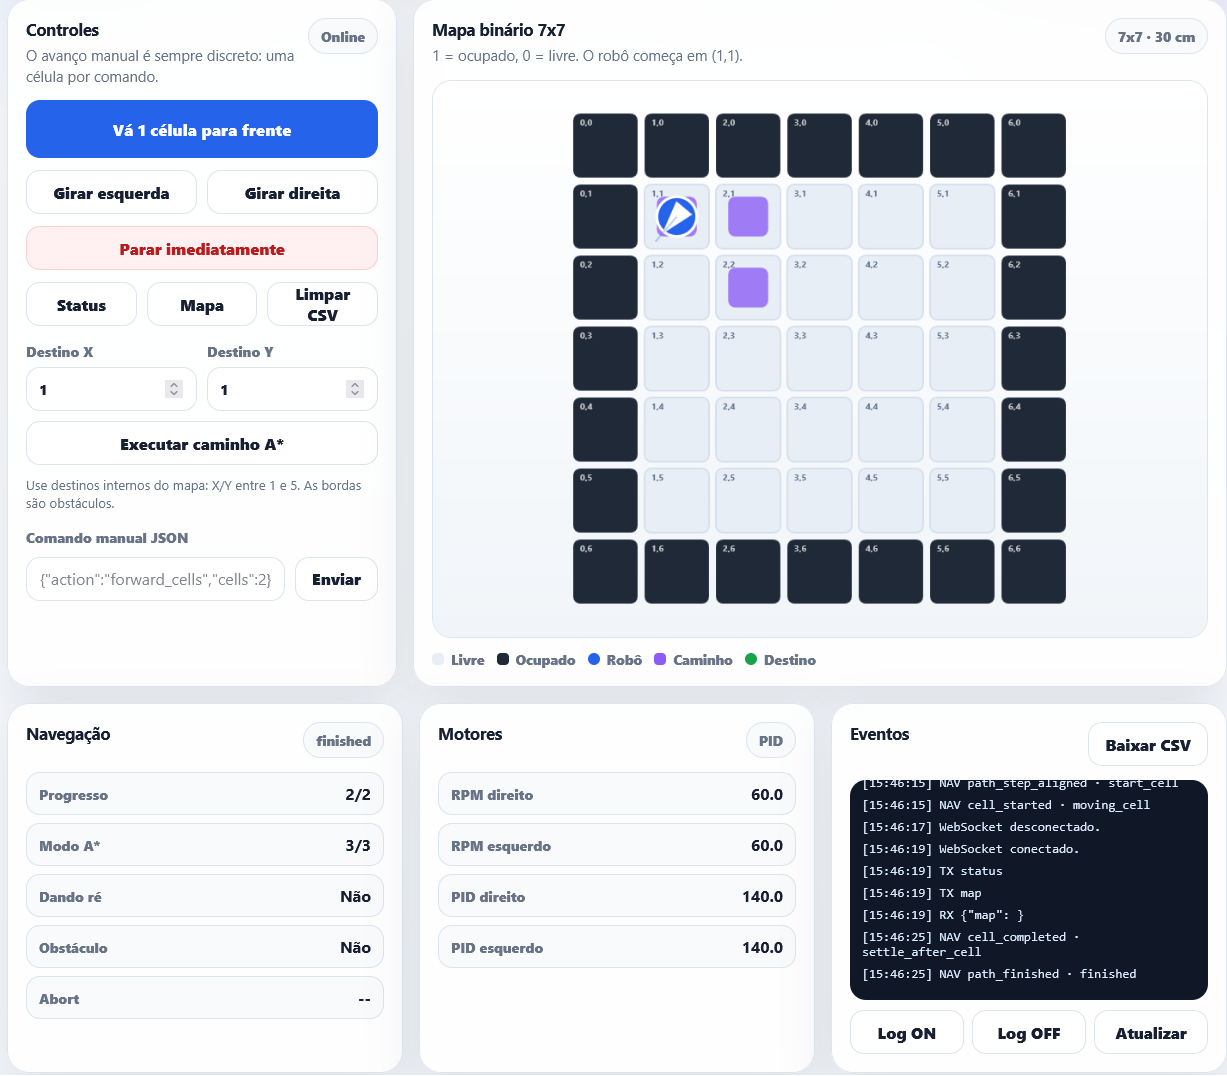
\includegraphics[width=0.9\linewidth]{imagens/Interface_Controle.png}
	\caption{Interface principal de controle do robô durante os testes.}
	\label{fig:interface-controle-resultados}
\end{figure}

A interface apresentada na Figura~\ref{fig:interface-controle-resultados} foi importante para a validação experimental porque permitiu comparar o comportamento físico do robô com a representação lógica exibida no mapa. Durante os testes, essa visualização ajudou a verificar se a célula estimada, a orientação e os comandos executados estavam coerentes com o comportamento esperado.

Além da interface principal, o sistema conta com uma tela de monitoramento e logs em tempo real. A Figura~\ref{fig:web-monitor-resultados} apresenta essa interface, utilizada para acompanhar mensagens do sistema durante a execução de comandos, deslocamentos, rotações e eventos de navegação.

\begin{figure}[H]
	\centering
	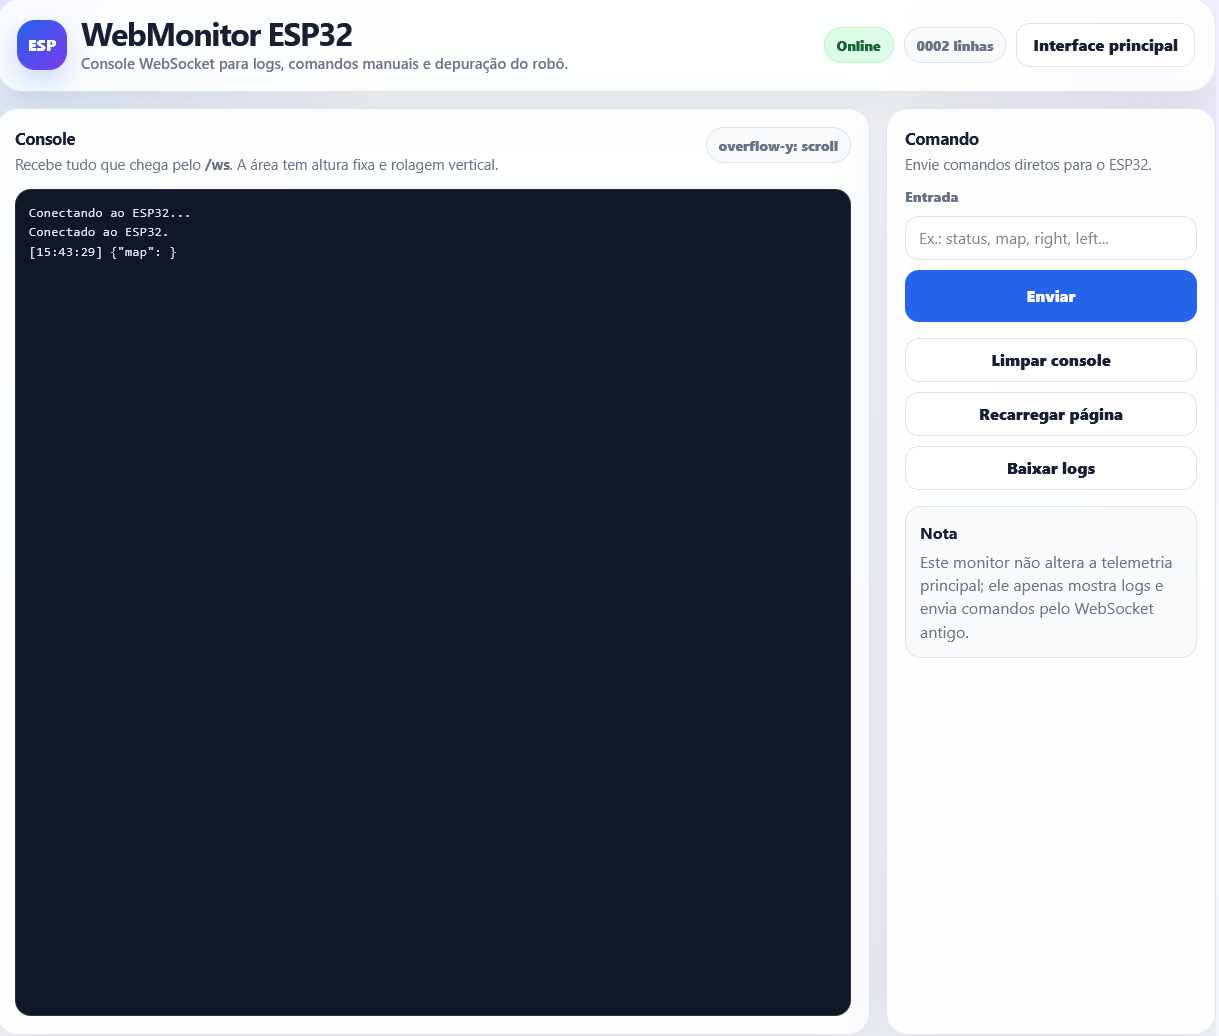
\includegraphics[width=0.9\linewidth]{imagens/Interface_WebTerminal.png}
	\caption{Interface de monitoramento e logs em tempo real.}
	\label{fig:web-monitor-resultados}
\end{figure}

A interface de monitoramento mostrada na Figura~\ref{fig:web-monitor-resultados} permitiu observar registros como início e fim de movimentos, conclusão de células, leituras de sensores, mensagens de obstáculo detectado, valores de rotação por encoder e informações de depuração. Esse recurso foi essencial para interpretar os resultados experimentais, pois muitos ajustes realizados no controle de movimento foram baseados nos registros exibidos durante os testes.

O monitor web também foi atualizado para apresentar aparência semelhante ao painel de controle e limitar a expansão do console de logs, utilizando rolagem vertical. Essa modificação foi necessária porque os testes geram grande volume de mensagens, principalmente durante curvas e navegação por múltiplas células. Com a limitação visual do console, a interface permanece utilizável mesmo durante execuções longas.

\section{Síntese dos Resultados Obtidos}
\label{sec:sintese_resultados_obtidos}

A síntese dos resultados destaca os módulos testados individualmente e a validação do planejamento de rotas com o algoritmo A* modificado. Esse ponto é importante porque o planejamento em grade representa uma das principais funcionalidades do sistema: gerar uma rota a partir de uma posição inicial e um destino definido, convertendo essa rota em comandos executáveis pelo robô.

Para demonstrar o funcionamento do A* modificado, foram considerados dois exemplos de destino a partir da mesma posição inicial \((1,1)\). O primeiro exemplo utiliza um destino alinhado com a posição inicial, enquanto o segundo utiliza um destino que exige mudança de direção. Essa comparação permite verificar tanto o cálculo de rotas simples quanto o comportamento do planejador em trajetórias com curvas.

% FIXME: Confirmar se os destinos abaixo foram utilizados nos testes reais.
% Caso os testes tenham usado outros destinos, substituir os pontos finais e as rotas calculadas pelos valores reais obtidos nos logs.

No primeiro exemplo, foi definida a posição inicial \((1,1)\) e a posição final \((5,1)\). Nesse caso, a rota planejada pelo A* modificado é predominantemente linear:

\begin{equation}
	R_1 = \{(1,1), (2,1), (3,1), (4,1), (5,1)\}
	\label{eq:rota_astar_exemplo_1}
\end{equation}

Essa rota possui quatro transições entre células e não exige mudança de direção, sendo adequada para verificar se o planejador gera corretamente um caminho direto quando não há obstáculos intermediários.

No segundo exemplo, foi definida a mesma posição inicial \((1,1)\), porém com posição final \((5,5)\). Nesse caso, a rota exige deslocamento em dois eixos do mapa. Considerando a penalização de curvas, o A* modificado tende a favorecer uma trajetória com menor número de mudanças de direção, como:

\begin{equation}
	R_2 = \{(1,1), (2,1), (3,1), (4,1), (5,1), (5,2), (5,3), (5,4), (5,5)\}
	\label{eq:rota_astar_exemplo_2}
\end{equation}

Essa segunda rota possui oito transições entre células e uma mudança principal de direção. O resultado é compatível com a proposta de penalizar curvas, pois o planejador evita trajetórias com alternância excessiva entre movimentos horizontais e verticais.

% TODO: Inserir figura ou captura da interface mostrando a rota \(R_1\) planejada no mapa.
% Sugestão de arquivo: imagens/rota_astar_exemplo_1.png

% TODO: Inserir figura ou captura da interface mostrando a rota \(R_2\) planejada no mapa.
% Sugestão de arquivo: imagens/rota_astar_exemplo_2.png

% TODO: Inserir imagem ou sequência de imagens do robô seguindo uma das rotas planejadas.
% Sugestão de arquivo: imagens/robo_executando_rota_astar.png

% TODO: Gravar vídeo do robô executando uma rota planejada pelo A* modificado para apresentação na defesa.
% Sugestão: mostrar a interface web ao lado do robô ou gravar primeiro a rota na interface e depois o robô executando o trajeto.

A Tabela~\ref{tab:exemplos_rotas_astar} resume os dois exemplos de rota calculados pelo A* modificado, destacando a posição inicial, a posição final, o número de células percorridas e a quantidade de mudanças de direção.

\begin{table}[H]
	\centering
	\caption{Exemplos de rotas calculadas pelo A* modificado.}
	\label{tab:exemplos_rotas_astar}
	\begin{tabular}{c c c c c}
		\hline
		\textbf{Exemplo} & \textbf{Início} & \textbf{Destino} & \textbf{Transições} & \textbf{Mudanças de direção} \\
		\hline
		\(R_1\) & \((1,1)\) & \((5,1)\) & 4 & 0 \\
		\(R_2\) & \((1,1)\) & \((5,5)\) & 8 & 1 \\
		\hline
	\end{tabular}
\end{table}

A Tabela~\ref{tab:exemplos_rotas_astar} evidencia que o planejador é capaz de gerar rotas válidas entre pontos distintos do mapa. Além disso, o segundo exemplo mostra o efeito da penalização de curvas, pois a rota resultante concentra a mudança de direção em um único ponto, favorecendo uma execução mais simples para o robô físico.

% FIXME: Comparar os exemplos da Tabela~\ref{tab:exemplos_rotas_astar} com os logs reais do sistema.
% Inserir, se possível, o caminho exatamente como foi impresso pela interface ou pelo monitor serial.

A Tabela~\ref{tab:sintese-resultados} sintetiza os principais resultados obtidos até o momento, considerando deslocamento linear, rotação, sensores, interface web e planejamento de rotas.

\begin{table}[H]
	\centering
	\caption{Síntese dos resultados experimentais do protótipo.}
	\label{tab:sintese-resultados}
	\begin{tabular}{p{3.4cm} p{4.8cm} p{4.9cm}}
		\hline
		\textbf{Módulo avaliado} & \textbf{Resultado obtido} & \textbf{Situação atual} \\
		\hline
		Deslocamento linear & Células próximas de \(0{,}30\,\text{m}\), com registros típicos entre \(0{,}286\,\text{m}\) e \(0{,}296\,\text{m}\) & Funcional, com necessidade de calibração fina \\
		Rotação & Controle por encoder tornou-se mais confiável após uso de \texttt{TURN\_ENCODER\_SCALE} & Funcional em desenvolvimento; fase fina precisa ajuste \\
		QMC5883L & Leituras instáveis durante motores ligados, com saltos de heading & Usado apenas como referência auxiliar filtrada \\
		VL53L0X & A detecção frontal interrompeu os motores e abortou a execução atual, conforme discutido na Seção~\ref{sec:resultado_deteccao_obstaculos} & Funcional como camada reativa de segurança \\
		Mapa 7x7 e A* modificado & Rotas foram geradas a partir de destinos distintos, com penalização de curvas e conversão em comandos de movimento & Planejamento e conversão lógica validados; a execução física deve ser discutida apenas com base nos ensaios registrados \\
		Interface web & Permitiu controle, telemetria, visualização de mapa, posição estimada e logs & Funcional, com melhorias visuais implementadas \\
		\hline
	\end{tabular}
\end{table}

A Tabela~\ref{tab:sintese-resultados} resume o estágio funcional atingido pelo protótipo. Os resultados demonstram que o sistema alcançou integração entre planejamento, controle de movimento, sensoriamento e interface web. O deslocamento linear apresentou medições próximas ao tamanho das células do grid, o controle de rotação evoluiu com a adoção da escala por encoder, o VL53L0X atuou como camada de segurança para detecção de obstáculos e a interface web permitiu acompanhar a navegação em tempo real.

O ponto mais importante para a validação do sistema integrado é o funcionamento do A* modificado em conjunto com a execução física da rota. Os exemplos \(R_1\) e \(R_2\) demonstram que o sistema gera caminhos a partir de destinos distintos e transforma cada sequência de células em comandos de movimento. Os registros visuais efetivamente disponíveis devem ser incluídos para relacionar o planejamento exibido na interface com a execução observada no protótipo.

% FIXME: Manter nesta seção apenas capturas e vídeos provenientes de ensaios realmente executados. Caso não exista registro da execução física completa de uma das rotas, declarar explicitamente que a validação correspondente se limitou ao planejamento e à geração dos comandos.

\chapter{Conclusão}

Este trabalho apresentou o desenvolvimento de um veículo robótico autônomo de pequeno porte baseado no microcontrolador ESP32, com foco na construção de uma plataforma de baixo custo, modular e adequada à navegação em ambientes internos. A proposta envolveu a integração de sensores, atuadores, algoritmos de controle, planejamento de rotas e uma interface web embarcada, buscando validar uma arquitetura funcional para deslocamento autônomo em um ambiente discretizado por células.

Ao longo do desenvolvimento, foi possível implementar uma arquitetura embarcada capaz de integrar motores DC, encoders ópticos, sensor de distância VL53L0X, magnetômetro QMC5883L, módulo Ponte H L298N e comunicação Wi-Fi por meio do ESP32. A utilização do PlatformIO e da estrutura modular do firmware favoreceu a organização do código e a separação das responsabilidades entre os diferentes módulos do sistema, como controle dos motores, leitura dos sensores, navegação, mapeamento, comunicação e interface com o usuário. Além disso, o uso de recursos de execução concorrente com FreeRTOS permitiu organizar rotinas paralelas de controle, telemetria e sensoriamento, reduzindo o risco de bloqueios durante a operação do robô.

A interface web embarcada também se mostrou um elemento importante para a operação e depuração do sistema. Por meio dela, foi possível enviar comandos, selecionar destinos no mapa, visualizar a posição estimada do robô, acompanhar a orientação e monitorar eventos registrados durante os testes. A adoção de WebSockets contribuiu para uma comunicação bidirecional em tempo real entre o navegador e o ESP32, permitindo maior responsividade durante a execução das rotinas de navegação.

Os resultados obtidos indicaram que o sistema foi capaz de executar deslocamentos lineares por células com desempenho compatível com o modelo adotado no projeto. Os testes com células de aproximadamente 30 cm demonstraram que o controle de avanço baseado em encoders apresentou comportamento consistente, permitindo ao robô percorrer trechos discretizados do mapa e fixar sua posição lógica após a conclusão de cada célula. Essa estratégia foi importante para reduzir o acúmulo de erro e manter a navegação coerente com a representação matricial do ambiente.

No controle de rotação, os testes evidenciaram a necessidade de calibração específica para a conversão entre a rotação estimada pelos encoders e o giro efetivo do robô. A introdução do fator \texttt{TURN\_ENCODER\_SCALE} permitiu ajustar a relação entre a leitura dos encoders e o ângulo executado, tornando o controle de curvas mais previsível. Além disso, a implementação de mecanismos de rejeição de leituras anômalas contribuiu para aumentar a robustez do sistema diante de variações abruptas ou inconsistências nas leituras de rotação.

A avaliação do magnetômetro QMC5883L mostrou que, embora o sensor seja útil como referência auxiliar de orientação em condições estáveis, suas leituras apresentaram elevada sensibilidade a interferências durante o acionamento dos motores. Foram observados saltos abruptos no \textit{heading} magnético, indicando que o magnetômetro não deve ser utilizado como principal referência para controle angular durante o movimento. Essa constatação levou à adoção de uma estratégia mais robusta, na qual os encoders são priorizados para a estimativa de deslocamento e rotação, enquanto o QMC5883L permanece como uma referência complementar, utilizada apenas quando suas leituras apresentam estabilidade suficiente.

O sensor VL53L0X foi integrado ao sistema com a finalidade de contribuir para a detecção de obstáculos e para a segurança da navegação. Embora a montagem física provisória tenha limitado seu posicionamento ideal durante parte dos testes, sua integração funcional com o firmware permitiu validar a leitura de distância e a lógica de interrupção da navegação quando um obstáculo era identificado. Dessa forma, o sensor demonstrou potencial para atuar como camada de segurança complementar ao planejamento de rotas e à navegação baseada em grid.

A metodologia de navegação utilizando mapa de ocupação 7x7 e planejamento de rota com algoritmo A* mostrou-se adequada para validar o funcionamento do protótipo em ambiente controlado. A representação do espaço por células simplificou a modelagem do ambiente e permitiu converter o caminho planejado em comandos discretos de movimentação. Essa abordagem, embora limitada em relação à complexidade de ambientes reais, mostrou-se suficiente para os objetivos deste trabalho, principalmente por permitir avaliar a integração entre planejamento, controle de movimento, sensoriamento e interface com o usuário.

Apesar dos resultados positivos, o projeto apresentou limitações relevantes. A montagem em protoboard e o uso de conectores jumper introduziram fragilidade mecânica e possibilidade de mau contato durante a movimentação. A interferência eletromagnética sobre o magnetômetro também se mostrou um fator significativo, reforçando a necessidade de melhor posicionamento físico dos sensores e de uma organização elétrica mais robusta. Além disso, a validação experimental foi realizada em ambiente controlado, com número limitado de repetições e com um mapa simplificado, o que restringe a generalização dos resultados para cenários mais complexos.

Ainda assim, o protótipo desenvolvido atingiu os principais objetivos propostos. Foi possível construir uma plataforma funcional, baseada em ESP32, capaz de integrar sensoriamento, controle de motores, planejamento de rotas, navegação por células e interface web embarcada. O trabalho também permitiu identificar, por meio dos testes, decisões importantes de arquitetura, como a priorização dos encoders para controle de movimentação, o uso do magnetômetro apenas como referência auxiliar e a necessidade de melhorias mecânicas para aumentar a confiabilidade do sistema.

Dessa forma, conclui-se que o projeto apresenta uma base viável para o desenvolvimento de robôs móveis autônomos de pequeno porte em contextos acadêmicos e educacionais. A arquitetura proposta é modular, expansível e compatível com futuras melhorias de hardware e software. Além de atender ao objetivo de construir um protótipo funcional, o trabalho contribuiu para consolidar conhecimentos relacionados a sistemas embarcados, robótica móvel, controle PID, odometria, sensoriamento, comunicação em tempo real e planejamento de trajetórias.

\section{Próximos Passos}

Como continuidade deste trabalho, recomenda-se, inicialmente, substituir a montagem em protoboard por uma placa de circuito impresso ou por uma placa de suporte mais robusta, com conectores adequados e melhor fixação mecânica dos módulos. Essa alteração tende a reduzir problemas de mau contato, interferência, vibração e desconexão durante os testes, aumentando a confiabilidade do protótipo.

Outro ponto importante consiste no reposicionamento definitivo do sensor VL53L0X na região frontal do robô, com suporte mecânico apropriado. Com essa fixação, será possível realizar testes mais precisos de detecção de obstáculos à frente do robô, avaliando a distância real de detecção, a repetibilidade das leituras e a resposta do sistema em diferentes condições de navegação. Essa melhoria também permitirá utilizar o sensor de forma mais efetiva na atualização dinâmica do mapa e na prevenção de colisões.

Também se recomenda a realização de novos testes com o magnetômetro QMC5883L afastado fisicamente da Ponte H, dos cabos de alimentação dos motores e de outras possíveis fontes de interferência eletromagnética. Essa avaliação permitirá verificar se a instabilidade observada nas leituras de \textit{heading} está associada principalmente ao posicionamento físico do sensor ou se decorre de limitações próprias do uso de magnetômetros em plataformas móveis com motores DC. Caso necessário, pode-se avaliar a substituição ou complementação do magnetômetro por uma unidade de medição inercial com giroscópio.

Em relação ao controle de movimento, trabalhos futuros podem aprofundar a calibração dos parâmetros PID e do fator de escala utilizado no controle de rotação. Para isso, recomenda-se a realização de ensaios repetidos de avanço, ré e curvas em diferentes ângulos, registrando o erro médio, o desvio padrão, o tempo de execução e a ocorrência de escorregamento das rodas. Esses dados permitiriam uma avaliação quantitativa mais rigorosa do desempenho do sistema e poderiam fundamentar ajustes mais precisos nos controladores.

A navegação também pode ser expandida por meio da implementação de atualização dinâmica do mapa de ocupação. Na versão atual, o mapa é utilizado principalmente como referência estática para planejamento de rotas e validação da navegação por células. Em versões futuras, as leituras do sensor de distância poderiam atualizar o estado das células em tempo real, permitindo que o robô replaneje trajetórias automaticamente quando obstáculos inesperados forem detectados.

Outra possibilidade de evolução consiste na melhoria da interface web, incluindo recursos de calibração diretamente pelo navegador, visualização gráfica dos logs, exportação dos dados dos testes e configuração de parâmetros como ganhos PID, escala de giro, tamanho da célula e limites de detecção de obstáculos. Esses recursos facilitariam a realização de ensaios experimentais e tornariam o sistema mais acessível para uso educacional e manutenção.

Por fim, recomenda-se ampliar a bateria de testes em ambientes físicos mais próximos de uma aplicação real, como corredores, salas e laboratórios. Esses testes devem considerar diferentes superfícies, níveis de iluminação, obstáculos estáticos e variações na posição inicial do robô. Com essas melhorias, o sistema poderá evoluir de um protótipo funcional validado em ambiente controlado para uma plataforma mais robusta de navegação autônoma em ambientes internos.

% ----------------------------------------------------------
% Referências bibliográficas
% ----------------------------------------------------------
% \bibliographystyle{plain}
\bibliography{references}

% ----------------------------------------------------------
% Glossário
% ----------------------------------------------------------
%
% Consulte o manual da classe abntex2 para orientações sobre o glossário.
%
%\glossary

% ----------------------------------------------------------
% Apêndices
% ----------------------------------------------------------


\end{document}
